%%%%%%%%%%%%%%%%%%%%%%%%%%%%%%%%%%%%%%%%%
% Masters/Doctoral Thesis 
% LaTeX Template
% Version 2.5 (27/8/17)
%
% This template was downloaded from:
% http://www.LaTeXTemplates.com
%
% Version 2.x major modifications by:
% Vel (vel@latextemplates.com)
%
% This template is based on a template by:
% Steve Gunn (http://users.ecs.soton.ac.uk/srg/softwaretools/document/templates/)
% Sunil Patel (http://www.sunilpatel.co.uk/thesis-template/)
%
% Template license:
% CC BY-NC-SA 3.0 (http://creativecommons.org/licenses/by-nc-sa/3.0/)
%
%%%%%%%%%%%%%%%%%%%%%%%%%%%%%%%%%%%%%%%%%

%----------------------------------------------------------------------------------------
%	PACKAGES AND OTHER DOCUMENT CONFIGURATIONS
%----------------------------------------------------------------------------------------

\documentclass[
11pt, % The default document font size, options: 10pt, 11pt, 12pt
%oneside, % Two side (alternating margins) for binding by default, uncomment to switch to one side
ngerman, % ngerman for German
singlespacing, % Single line spacing, alternatives: onehalfspacing or doublespacing
%draft, % Uncomment to enable draft mode (no pictures, no links, overfull hboxes indicated)
%nolistspacing, % If the document is onehalfspacing or doublespacing, uncomment this to set spacing in lists to single
%liststotoc, % Uncomment to add the list of figures/tables/etc to the table of contents
%toctotoc, % Uncomment to add the main table of contents to the table of contents
%parskip, % Uncomment to add space between paragraphs
%nohyperref, % Uncomment to not load the hyperref package
headsepline, % Uncomment to get a line under the header
%chapterinoneline, % Uncomment to place the chapter title next to the number on one line
%consistentlayout, % Uncomment to change the layout of the declaration, abstract and acknowledgements pages to match the default layout
]{MastersDoctoralThesis} % The class file specifying the document structure

\usepackage[utf8]{inputenc} % Required for inputting international characters
\usepackage[T1]{fontenc} % Output font encoding for international characters

\usepackage{mathpazo} % Use the Palatino font by default

\usepackage[backend=bibtex,style=authoryear,natbib=true]{biblatex} % Use the bibtex backend with the authoryear citation style (which resembles APA)

\addbibresource{example.bib} % The filename of the bibliography

\usepackage[autostyle=true]{csquotes} % Required to generate language-dependent quotes in the bibliography

%----------------------------------------------------------------------------------------
%	MARGIN SETTINGS
%----------------------------------------------------------------------------------------

\geometry{
	paper=a4paper, % Change to letterpaper for US letter
	inner=2.5cm, % Inner margin
	outer=3.8cm, % Outer margin
	bindingoffset=.5cm, % Binding offset
	top=1.5cm, % Top margin
	bottom=1.5cm, % Bottom margin
	%showframe, % Uncomment to show how the type block is set on the page
}

%----------------------------------------------------------------------------------------
%	THESIS INFORMATION
%----------------------------------------------------------------------------------------

\thesistitle{Analyse dünnbesetzter Hauptachsen für Frequenzdaten} % Your thesis title, this is used in the title and abstract, print it elsewhere with \ttitle
\supervisor{Prof. Dr. Jochen \textsc{Garcke}} % Your supervisor's name, this is used in the title page, print it elsewhere with \supname
\examiner{} % Your examiner's name, this is not currently used anywhere in the template, print it elsewhere with \examname
\degree{Bachelor of Science} % Your degree name, this is used in the title page and abstract, print it elsewhere with \degreename
\author{Tobias \textsc{Bork}} % Your name, this is used in the title page and abstract, print it elsewhere with \authorname
\addresses{} % Your address, this is not currently used anywhere in the template, print it elsewhere with \addressname

\subject{Machine Learning} % Your subject area, this is not currently used anywhere in the template, print it elsewhere with \subjectname
\keywords{} % Keywords for your thesis, this is not currently used anywhere in the template, print it elsewhere with \keywordnames
\university{\href{https://www.uni-bonn.de/}{Rheinische Friedrich-Wilhelms-Universität Bonn}} % Your university's name and URL, this is used in the title page and abstract, print it elsewhere with \univname
\department{\href{https://www.math.uni-bonn.de/}{Mathematisches Institut}} % Your department's name and URL, this is used in the title page and abstract, print it elsewhere with \deptname
\group{\href{https://www.scai.fraunhofer.de/de/geschaeftsfelder/numerische-datenbasierte-vorhersage.html}{Numerische Datenbasierte Vorhersage, Fraunofer SCAI}} % Your research group's name and URL, this is used in the title page, print it elsewhere with \groupname
\faculty{\href{https://ins.uni-bonn.de/}{Institut für Numerische Simulation}} % Your faculty's name and URL, this is used in the title page and abstract, print it elsewhere with \facname

\AtBeginDocument{
\hypersetup{pdftitle=\ttitle} % Set the PDF's title to your title
\hypersetup{pdfauthor=\authorname} % Set the PDF's author to your name
\hypersetup{pdfkeywords=\keywordnames} % Set the PDF's keywords to your keywords
}

\begin{document}

\frontmatter % Use roman page numbering style (i, ii, iii, iv...) for the pre-content pages

\pagestyle{plain} % Default to the plain heading style until the thesis style is called for the body content

%----------------------------------------------------------------------------------------
%	TITLE PAGE
%----------------------------------------------------------------------------------------

\begin{titlepage}
\begin{center}

\vspace*{.06\textheight}
{\scshape\LARGE \univname\par}\vspace{1.5cm} % University name
\textsc{\Large Bachelorarbeit}\\[0.5cm] % Thesis type

\HRule \\[0.4cm] % Horizontal line
{\huge \bfseries \ttitle\par}\vspace{0.4cm} % Thesis title
\HRule \\[1.5cm] % Horizontal line
 
\begin{minipage}[t]{0.4\textwidth}
\begin{flushleft} \large
\emph{Autor:}\\
\href{https://www.uni-bonn.de/}{\authorname} % Author name - remove the \href bracket to remove the link
\end{flushleft}
\end{minipage}
\begin{minipage}[t]{0.4\textwidth}
\begin{flushright} \large
\emph{Betreuer:} \\
\href{https://ins.uni-bonn.de/staff/garcke}{\supname} % Supervisor name - remove the \href bracket to remove the link  
\end{flushright}
\end{minipage}\\[3cm]
 
\vfill

\large \textit{A thesis submitted in fulfillment of the requirements\\ for the degree of \degreename}\\[0.3cm] % University requirement text
\textit{in the}\\[0.4cm]
\facname\\\groupname\\[2cm] % Research group name and department name
 
\vfill

{\large \today}\\[4cm] % Date
%\includegraphics{Logo} % University/department logo - uncomment to place it
 
\vfill
\end{center}
\end{titlepage}

%----------------------------------------------------------------------------------------
%	DECLARATION PAGE
%----------------------------------------------------------------------------------------

\begin{declaration}
\addchaptertocentry{\authorshipname} % Add the declaration to the table of contents
\noindent I, \authorname, declare that this thesis titled, \enquote{\ttitle} and the work presented in it are my own. I confirm that:

\begin{itemize} 
\item This work was done wholly or mainly while in candidature for a research degree at this University.
\item Where any part of this thesis has previously been submitted for a degree or any other qualification at this University or any other institution, this has been clearly stated.
\item Where I have consulted the published work of others, this is always clearly attributed.
\item Where I have quoted from the work of others, the source is always given. With the exception of such quotations, this thesis is entirely my own work.
\item I have acknowledged all main sources of help.
\item Where the thesis is based on work done by myself jointly with others, I have made clear exactly what was done by others and what I have contributed myself.\\
\end{itemize}
 
\noindent Signed:\\
\rule[0.5em]{25em}{0.5pt} % This prints a line for the signature
 
\noindent Date:\\
\rule[0.5em]{25em}{0.5pt} % This prints a line to write the date
\end{declaration}

\cleardoublepage

%----------------------------------------------------------------------------------------
%	QUOTATION PAGE
%----------------------------------------------------------------------------------------

\vspace*{0.2\textheight}

\noindent\enquote{\itshape Thanks to my solid academic training, today I can write hundreds of words on virtually any topic without possessing a shred of information, which is how I got a good job in journalism.}\bigbreak

\hfill Dave Barry

%----------------------------------------------------------------------------------------
%	ABSTRACT PAGE
%----------------------------------------------------------------------------------------

\begin{abstract}
\addchaptertocentry{\abstractname} % Add the abstract to the table of contents
The Thesis Abstract is written here (and usually kept to just this page). The page is kept centered vertically so can expand into the blank space above the title too\ldots
\end{abstract}

%----------------------------------------------------------------------------------------
%	ACKNOWLEDGEMENTS
%----------------------------------------------------------------------------------------

\begin{acknowledgements}
\addchaptertocentry{\acknowledgementname} % Add the acknowledgements to the table of contents
The acknowledgments and the people to thank go here, don't forget to include your project advisor\ldots
\end{acknowledgements}

%----------------------------------------------------------------------------------------
%	LIST OF CONTENTS/FIGURES/TABLES PAGES
%----------------------------------------------------------------------------------------

\tableofcontents % Prints the main table of contents

\listoffigures % Prints the list of figures

\listoftables % Prints the list of tables

%----------------------------------------------------------------------------------------
%	ABBREVIATIONS
%----------------------------------------------------------------------------------------

\begin{abbreviations}{ll} % Include a list of abbreviations (a table of two columns)

\textbf{LAH} & \textbf{L}ist \textbf{A}bbreviations \textbf{H}ere\\
\textbf{WSF} & \textbf{W}hat (it) \textbf{S}tands \textbf{F}or\\

\end{abbreviations}


%----------------------------------------------------------------------------------------
%	SYMBOLS
%----------------------------------------------------------------------------------------

\begin{symbols}{lll} % Include a list of Symbols (a three column table)

$a$ & distance & \si{\meter} \\
$P$ & power & \si{\watt} (\si{\joule\per\second}) \\
%Symbol & Name & Unit \\

\addlinespace % Gap to separate the Roman symbols from the Greek

$\omega$ & angular frequency & \si{\radian} \\

\end{symbols}

%----------------------------------------------------------------------------------------
%	DEDICATION
%----------------------------------------------------------------------------------------

\dedicatory{For/Dedicated to/To my\ldots} 

%----------------------------------------------------------------------------------------
%	THESIS CONTENT - CHAPTERS
%----------------------------------------------------------------------------------------

\mainmatter % Begin numeric (1,2,3...) page numbering

\pagestyle{thesis} % Return the page headers back to the "thesis" style

% Include the chapters of the thesis as separate files from the Chapters folder
% Uncomment the lines as you write the chapters

% Chapter 1

\chapter{Chapter Title Here} % Main chapter title

\label{Chapter1} % For referencing the chapter elsewhere, use \ref{Chapter1} 

%----------------------------------------------------------------------------------------

% Define some commands to keep the formatting separated from the content 
\newcommand{\keyword}[1]{\textbf{#1}}
\newcommand{\tabhead}[1]{\textbf{#1}}
\newcommand{\code}[1]{\texttt{#1}}
\newcommand{\file}[1]{\texttt{\bfseries#1}}
\newcommand{\option}[1]{\texttt{\itshape#1}}

%----------------------------------------------------------------------------------------

\section{Welcome and Thank You}
Welcome to this \LaTeX{} Thesis Template, a beautiful and easy to use template for writing a thesis using the \LaTeX{} typesetting system.

If you are writing a thesis (or will be in the future) and its subject is technical or mathematical (though it doesn't have to be), then creating it in \LaTeX{} is highly recommended as a way to make sure you can just get down to the essential writing without having to worry over formatting or wasting time arguing with your word processor.

\LaTeX{} is easily able to professionally typeset documents that run to hundreds or thousands of pages long. With simple mark-up commands, it automatically sets out the table of contents, margins, page headers and footers and keeps the formatting consistent and beautiful. One of its main strengths is the way it can easily typeset mathematics, even \emph{heavy} mathematics. Even if those equations are the most horribly twisted and most difficult mathematical problems that can only be solved on a super-computer, you can at least count on \LaTeX{} to make them look stunning.

%----------------------------------------------------------------------------------------

\section{Learning \LaTeX{}}

\LaTeX{} is not a \textsc{wysiwyg} (What You See is What You Get) program, unlike word processors such as Microsoft Word or Apple's Pages. Instead, a document written for \LaTeX{} is actually a simple, plain text file that contains \emph{no formatting}. You tell \LaTeX{} how you want the formatting in the finished document by writing in simple commands amongst the text, for example, if I want to use \emph{italic text for emphasis}, I write the \verb|\emph{text}| command and put the text I want in italics in between the curly braces. This means that \LaTeX{} is a \enquote{mark-up} language, very much like HTML.

\subsection{A (not so short) Introduction to \LaTeX{}}

If you are new to \LaTeX{}, there is a very good eBook -- freely available online as a PDF file -- called, \enquote{The Not So Short Introduction to \LaTeX{}}. The book's title is typically shortened to just \emph{lshort}. You can download the latest version (as it is occasionally updated) from here:
\url{http://www.ctan.org/tex-archive/info/lshort/english/lshort.pdf}

It is also available in several other languages. Find yours from the list on this page: \url{http://www.ctan.org/tex-archive/info/lshort/}

It is recommended to take a little time out to learn how to use \LaTeX{} by creating several, small `test' documents, or having a close look at several templates on:\\ 
\url{http://www.LaTeXTemplates.com}\\ 
Making the effort now means you're not stuck learning the system when what you \emph{really} need to be doing is writing your thesis.

\subsection{A Short Math Guide for \LaTeX{}}

If you are writing a technical or mathematical thesis, then you may want to read the document by the AMS (American Mathematical Society) called, \enquote{A Short Math Guide for \LaTeX{}}. It can be found online here:
\url{http://www.ams.org/tex/amslatex.html}
under the \enquote{Additional Documentation} section towards the bottom of the page.

\subsection{Common \LaTeX{} Math Symbols}
There are a multitude of mathematical symbols available for \LaTeX{} and it would take a great effort to learn the commands for them all. The most common ones you are likely to use are shown on this page:
\url{http://www.sunilpatel.co.uk/latex-type/latex-math-symbols/}

You can use this page as a reference or crib sheet, the symbols are rendered as large, high quality images so you can quickly find the \LaTeX{} command for the symbol you need.

\subsection{\LaTeX{} on a Mac}
 
The \LaTeX{} distribution is available for many systems including Windows, Linux and Mac OS X. The package for OS X is called MacTeX and it contains all the applications you need -- bundled together and pre-customized -- for a fully working \LaTeX{} environment and work flow.
 
MacTeX includes a custom dedicated \LaTeX{} editor called TeXShop for writing your `\file{.tex}' files and BibDesk: a program to manage your references and create your bibliography section just as easily as managing songs and creating playlists in iTunes.

%----------------------------------------------------------------------------------------

\section{Getting Started with this Template}

If you are familiar with \LaTeX{}, then you should explore the directory structure of the template and then proceed to place your own information into the \emph{THESIS INFORMATION} block of the \file{main.tex} file. You can then modify the rest of this file to your unique specifications based on your degree/university. Section \ref{FillingFile} on page \pageref{FillingFile} will help you do this. Make sure you also read section \ref{ThesisConventions} about thesis conventions to get the most out of this template.

If you are new to \LaTeX{} it is recommended that you carry on reading through the rest of the information in this document.

Before you begin using this template you should ensure that its style complies with the thesis style guidelines imposed by your institution. In most cases this template style and layout will be suitable. If it is not, it may only require a small change to bring the template in line with your institution's recommendations. These modifications will need to be done on the \file{MastersDoctoralThesis.cls} file.

\subsection{About this Template}

This \LaTeX{} Thesis Template is originally based and created around a \LaTeX{} style file created by Steve R.\ Gunn from the University of Southampton (UK), department of Electronics and Computer Science. You can find his original thesis style file at his site, here:
\url{http://www.ecs.soton.ac.uk/~srg/softwaretools/document/templates/}

Steve's \file{ecsthesis.cls} was then taken by Sunil Patel who modified it by creating a skeleton framework and folder structure to place the thesis files in. The resulting template can be found on Sunil's site here:
\url{http://www.sunilpatel.co.uk/thesis-template}

Sunil's template was made available through \url{http://www.LaTeXTemplates.com} where it was modified many times based on user requests and questions. Version 2.0 and onwards of this template represents a major modification to Sunil's template and is, in fact, hardly recognisable. The work to make version 2.0 possible was carried out by \href{mailto:vel@latextemplates.com}{Vel} and Johannes Böttcher.

%----------------------------------------------------------------------------------------

\section{What this Template Includes}

\subsection{Folders}

This template comes as a single zip file that expands out to several files and folders. The folder names are mostly self-explanatory:

\keyword{Appendices} -- this is the folder where you put the appendices. Each appendix should go into its own separate \file{.tex} file. An example and template are included in the directory.

\keyword{Chapters} -- this is the folder where you put the thesis chapters. A thesis usually has about six chapters, though there is no hard rule on this. Each chapter should go in its own separate \file{.tex} file and they can be split as:
\begin{itemize}
\item Chapter 1: Introduction to the thesis topic
\item Chapter 2: Background information and theory
\item Chapter 3: (Laboratory) experimental setup
\item Chapter 4: Details of experiment 1
\item Chapter 5: Details of experiment 2
\item Chapter 6: Discussion of the experimental results
\item Chapter 7: Conclusion and future directions
\end{itemize}
This chapter layout is specialised for the experimental sciences, your discipline may be different.

\keyword{Figures} -- this folder contains all figures for the thesis. These are the final images that will go into the thesis document.

\subsection{Files}

Included are also several files, most of them are plain text and you can see their contents in a text editor. After initial compilation, you will see that more auxiliary files are created by \LaTeX{} or BibTeX and which you don't need to delete or worry about:

\keyword{example.bib} -- this is an important file that contains all the bibliographic information and references that you will be citing in the thesis for use with BibTeX. You can write it manually, but there are reference manager programs available that will create and manage it for you. Bibliographies in \LaTeX{} are a large subject and you may need to read about BibTeX before starting with this. Many modern reference managers will allow you to export your references in BibTeX format which greatly eases the amount of work you have to do.

\keyword{MastersDoctoralThesis.cls} -- this is an important file. It is the class file that tells \LaTeX{} how to format the thesis. 

\keyword{main.pdf} -- this is your beautifully typeset thesis (in the PDF file format) created by \LaTeX{}. It is supplied in the PDF with the template and after you compile the template you should get an identical version.

\keyword{main.tex} -- this is an important file. This is the file that you tell \LaTeX{} to compile to produce your thesis as a PDF file. It contains the framework and constructs that tell \LaTeX{} how to layout the thesis. It is heavily commented so you can read exactly what each line of code does and why it is there. After you put your own information into the \emph{THESIS INFORMATION} block -- you have now started your thesis!

Files that are \emph{not} included, but are created by \LaTeX{} as auxiliary files include:

\keyword{main.aux} -- this is an auxiliary file generated by \LaTeX{}, if it is deleted \LaTeX{} simply regenerates it when you run the main \file{.tex} file.

\keyword{main.bbl} -- this is an auxiliary file generated by BibTeX, if it is deleted, BibTeX simply regenerates it when you run the \file{main.aux} file. Whereas the \file{.bib} file contains all the references you have, this \file{.bbl} file contains the references you have actually cited in the thesis and is used to build the bibliography section of the thesis.

\keyword{main.blg} -- this is an auxiliary file generated by BibTeX, if it is deleted BibTeX simply regenerates it when you run the main \file{.aux} file.

\keyword{main.lof} -- this is an auxiliary file generated by \LaTeX{}, if it is deleted \LaTeX{} simply regenerates it when you run the main \file{.tex} file. It tells \LaTeX{} how to build the \emph{List of Figures} section.

\keyword{main.log} -- this is an auxiliary file generated by \LaTeX{}, if it is deleted \LaTeX{} simply regenerates it when you run the main \file{.tex} file. It contains messages from \LaTeX{}, if you receive errors and warnings from \LaTeX{}, they will be in this \file{.log} file.

\keyword{main.lot} -- this is an auxiliary file generated by \LaTeX{}, if it is deleted \LaTeX{} simply regenerates it when you run the main \file{.tex} file. It tells \LaTeX{} how to build the \emph{List of Tables} section.

\keyword{main.out} -- this is an auxiliary file generated by \LaTeX{}, if it is deleted \LaTeX{} simply regenerates it when you run the main \file{.tex} file.

So from this long list, only the files with the \file{.bib}, \file{.cls} and \file{.tex} extensions are the most important ones. The other auxiliary files can be ignored or deleted as \LaTeX{} and BibTeX will regenerate them.

%----------------------------------------------------------------------------------------

\section{Filling in Your Information in the \file{main.tex} File}\label{FillingFile}

You will need to personalise the thesis template and make it your own by filling in your own information. This is done by editing the \file{main.tex} file in a text editor or your favourite LaTeX environment.

Open the file and scroll down to the third large block titled \emph{THESIS INFORMATION} where you can see the entries for \emph{University Name}, \emph{Department Name}, etc \ldots

Fill out the information about yourself, your group and institution. You can also insert web links, if you do, make sure you use the full URL, including the \code{http://} for this. If you don't want these to be linked, simply remove the \verb|\href{url}{name}| and only leave the name.

When you have done this, save the file and recompile \code{main.tex}. All the information you filled in should now be in the PDF, complete with web links. You can now begin your thesis proper!

%----------------------------------------------------------------------------------------

\section{The \code{main.tex} File Explained}

The \file{main.tex} file contains the structure of the thesis. There are plenty of written comments that explain what pages, sections and formatting the \LaTeX{} code is creating. Each major document element is divided into commented blocks with titles in all capitals to make it obvious what the following bit of code is doing. Initially there seems to be a lot of \LaTeX{} code, but this is all formatting, and it has all been taken care of so you don't have to do it.

Begin by checking that your information on the title page is correct. For the thesis declaration, your institution may insist on something different than the text given. If this is the case, just replace what you see with what is required in the \emph{DECLARATION PAGE} block.

Then comes a page which contains a funny quote. You can put your own, or quote your favourite scientist, author, person, and so on. Make sure to put the name of the person who you took the quote from.

Following this is the abstract page which summarises your work in a condensed way and can almost be used as a standalone document to describe what you have done. The text you write will cause the heading to move up so don't worry about running out of space.

Next come the acknowledgements. On this page, write about all the people who you wish to thank (not forgetting parents, partners and your advisor/supervisor).

The contents pages, list of figures and tables are all taken care of for you and do not need to be manually created or edited. The next set of pages are more likely to be optional and can be deleted since they are for a more technical thesis: insert a list of abbreviations you have used in the thesis, then a list of the physical constants and numbers you refer to and finally, a list of mathematical symbols used in any formulae. Making the effort to fill these tables means the reader has a one-stop place to refer to instead of searching the internet and references to try and find out what you meant by certain abbreviations or symbols.

The list of symbols is split into the Roman and Greek alphabets. Whereas the abbreviations and symbols ought to be listed in alphabetical order (and this is \emph{not} done automatically for you) the list of physical constants should be grouped into similar themes.

The next page contains a one line dedication. Who will you dedicate your thesis to?

Finally, there is the block where the chapters are included. Uncomment the lines (delete the \code{\%} character) as you write the chapters. Each chapter should be written in its own file and put into the \emph{Chapters} folder and named \file{Chapter1}, \file{Chapter2}, etc\ldots Similarly for the appendices, uncomment the lines as you need them. Each appendix should go into its own file and placed in the \emph{Appendices} folder.

After the preamble, chapters and appendices finally comes the bibliography. The bibliography style (called \option{authoryear}) is used for the bibliography and is a fully featured style that will even include links to where the referenced paper can be found online. Do not underestimate how grateful your reader will be to find that a reference to a paper is just a click away. Of course, this relies on you putting the URL information into the BibTeX file in the first place.

%----------------------------------------------------------------------------------------

\section{Thesis Features and Conventions}\label{ThesisConventions}

To get the best out of this template, there are a few conventions that you may want to follow.

One of the most important (and most difficult) things to keep track of in such a long document as a thesis is consistency. Using certain conventions and ways of doing things (such as using a Todo list) makes the job easier. Of course, all of these are optional and you can adopt your own method.

\subsection{Printing Format}

This thesis template is designed for double sided printing (i.e. content on the front and back of pages) as most theses are printed and bound this way. Switching to one sided printing is as simple as uncommenting the \option{oneside} option of the \code{documentclass} command at the top of the \file{main.tex} file. You may then wish to adjust the margins to suit specifications from your institution.

The headers for the pages contain the page number on the outer side (so it is easy to flick through to the page you want) and the chapter name on the inner side.

The text is set to 11 point by default with single line spacing, again, you can tune the text size and spacing should you want or need to using the options at the very start of \file{main.tex}. The spacing can be changed similarly by replacing the \option{singlespacing} with \option{onehalfspacing} or \option{doublespacing}.

\subsection{Using US Letter Paper}

The paper size used in the template is A4, which is the standard size in Europe. If you are using this thesis template elsewhere and particularly in the United States, then you may have to change the A4 paper size to the US Letter size. This can be done in the margins settings section in \file{main.tex}.

Due to the differences in the paper size, the resulting margins may be different to what you like or require (as it is common for institutions to dictate certain margin sizes). If this is the case, then the margin sizes can be tweaked by modifying the values in the same block as where you set the paper size. Now your document should be set up for US Letter paper size with suitable margins.

\subsection{References}

The \code{biblatex} package is used to format the bibliography and inserts references such as this one. The options used in the \file{main.tex} file mean that the in-text citations of references are formatted with the author(s) listed with the date of the publication. Multiple references are separated by semicolons (e.g. and references with more than three authors only show the first author with \emph{et al.} indicating there are more authors (e.g.). This is done automatically for you. To see how you use references, have a look at the \file{Chapter1.tex} source file. Many reference managers allow you to simply drag the reference into the document as you type.

Scientific references should come \emph{before} the punctuation mark if there is one (such as a comma or period). The same goes for footnotes\footnote{Such as this footnote, here down at the bottom of the page.}. You can change this but the most important thing is to keep the convention consistent throughout the thesis. Footnotes themselves should be full, descriptive sentences (beginning with a capital letter and ending with a full stop). The APA6 states: \enquote{Footnote numbers should be superscripted, [...], following any punctuation mark except a dash.} The Chicago manual of style states: \enquote{A note number should be placed at the end of a sentence or clause. The number follows any punctuation mark except the dash, which it precedes. It follows a closing parenthesis.}

The bibliography is typeset with references listed in alphabetical order by the first author's last name. This is similar to the APA referencing style. To see how \LaTeX{} typesets the bibliography, have a look at the very end of this document (or just click on the reference number links in in-text citations).

\subsubsection{A Note on bibtex}

The bibtex backend used in the template by default does not correctly handle unicode character encoding (i.e. "international" characters). You may see a warning about this in the compilation log and, if your references contain unicode characters, they may not show up correctly or at all. The solution to this is to use the biber backend instead of the outdated bibtex backend. This is done by finding this in \file{main.tex}: \option{backend=bibtex} and changing it to \option{backend=biber}. You will then need to delete all auxiliary BibTeX files and navigate to the template directory in your terminal (command prompt). Once there, simply type \code{biber main} and biber will compile your bibliography. You can then compile \file{main.tex} as normal and your bibliography will be updated. An alternative is to set up your LaTeX editor to compile with biber instead of bibtex, see \href{http://tex.stackexchange.com/questions/154751/biblatex-with-biber-configuring-my-editor-to-avoid-undefined-citations/}{here} for how to do this for various editors.

\subsection{Tables}

Tables are an important way of displaying your results, below is an example table which was generated with this code:

{\small
\begin{verbatim}
\begin{table}
\caption{The effects of treatments X and Y on the four groups studied.}
\label{tab:treatments}
\centering
\begin{tabular}{l l l}
\toprule
\tabhead{Groups} & \tabhead{Treatment X} & \tabhead{Treatment Y} \\
\midrule
1 & 0.2 & 0.8\\
2 & 0.17 & 0.7\\
3 & 0.24 & 0.75\\
4 & 0.68 & 0.3\\
\bottomrule\\
\end{tabular}
\end{table}
\end{verbatim}
}

\begin{table}
\caption{The effects of treatments X and Y on the four groups studied.}
\label{tab:treatments}
\centering
\begin{tabular}{l l l}
\toprule
\tabhead{Groups} & \tabhead{Treatment X} & \tabhead{Treatment Y} \\
\midrule
1 & 0.2 & 0.8\\
2 & 0.17 & 0.7\\
3 & 0.24 & 0.75\\
4 & 0.68 & 0.3\\
\bottomrule\\
\end{tabular}
\end{table}

You can reference tables with \verb|\ref{<label>}| where the label is defined within the table environment. See \file{Chapter1.tex} for an example of the label and citation (e.g. Table~\ref{tab:treatments}).

\subsection{Figures}

There will hopefully be many figures in your thesis (that should be placed in the \emph{Figures} folder). The way to insert figures into your thesis is to use a code template like this:
\begin{verbatim}
\begin{figure}
\centering

\includegraphics{figures/Electron}
\decoRule
\caption[An Electron]{An electron (artist's impression).}
\label{fig:Electron}
\end{figure}
\end{verbatim}
Also look in the source file. Putting this code into the source file produces the picture of the electron that you can see in the figure below.

\begin{figure}[th]
\centering
%
\includegraphics{figures/Electron}
\decoRule
\caption[An Electron]{An electron (artist's impression).}
\label{fig:Electron}
\end{figure}

Sometimes figures don't always appear where you write them in the source. The placement depends on how much space there is on the page for the figure. Sometimes there is not enough room to fit a figure directly where it should go (in relation to the text) and so \LaTeX{} puts it at the top of the next page. Positioning figures is the job of \LaTeX{} and so you should only worry about making them look good!

Figures usually should have captions just in case you need to refer to them (such as in Figure~\ref{fig:Electron}). The \verb|\caption| command contains two parts, the first part, inside the square brackets is the title that will appear in the \emph{List of Figures}, and so should be short. The second part in the curly brackets should contain the longer and more descriptive caption text.

The \verb|\decoRule| command is optional and simply puts an aesthetic horizontal line below the image. If you do this for one image, do it for all of them.

\LaTeX{} is capable of using images in pdf, jpg and png format.

\subsection{Typesetting mathematics}

If your thesis is going to contain heavy mathematical content, be sure that \LaTeX{} will make it look beautiful, even though it won't be able to solve the equations for you.

The \enquote{Not So Short Introduction to \LaTeX} (available on \href{http://www.ctan.org/tex-archive/info/lshort/english/lshort.pdf}{CTAN}) should tell you everything you need to know for most cases of typesetting mathematics. If you need more information, a much more thorough mathematical guide is available from the AMS called, \enquote{A Short Math Guide to \LaTeX} and can be downloaded from:
\url{ftp://ftp.ams.org/pub/tex/doc/amsmath/short-math-guide.pdf}

There are many different \LaTeX{} symbols to remember, luckily you can find the most common symbols in \href{http://ctan.org/pkg/comprehensive}{The Comprehensive \LaTeX~Symbol List}.

You can write an equation, which is automatically given an equation number by \LaTeX{} like this:
\begin{verbatim}
\begin{equation}
E = mc^{2}
\label{eqn:Einstein}
\end{equation}
\end{verbatim}

This will produce Einstein's famous energy-matter equivalence equation:
\begin{equation}
E = mc^{2}
\label{eqn:Einstein}
\end{equation}

All equations you write (which are not in the middle of paragraph text) are automatically given equation numbers by \LaTeX{}. If you don't want a particular equation numbered, use the unnumbered form:
\begin{verbatim}
\[ a^{2}=4 \]
\end{verbatim}

%----------------------------------------------------------------------------------------

\section{Sectioning and Subsectioning}

You should break your thesis up into nice, bite-sized sections and subsections. \LaTeX{} automatically builds a table of Contents by looking at all the \verb|\chapter{}|, \verb|\section{}|  and \verb|\subsection{}| commands you write in the source.

The Table of Contents should only list the sections to three (3) levels. A \verb|chapter{}| is level zero (0). A \verb|\section{}| is level one (1) and so a \verb|\subsection{}| is level two (2). In your thesis it is likely that you will even use a \verb|subsubsection{}|, which is level three (3). The depth to which the Table of Contents is formatted is set within \file{MastersDoctoralThesis.cls}. If you need this changed, you can do it in \file{main.tex}.

%----------------------------------------------------------------------------------------

\section{In Closing}

You have reached the end of this mini-guide. You can now rename or overwrite this pdf file and begin writing your own \file{Chapter1.tex} and the rest of your thesis. The easy work of setting up the structure and framework has been taken care of for you. It's now your job to fill it out!

Good luck and have lots of fun!

\begin{flushright}
Guide written by ---\\
Sunil Patel: \href{http://www.sunilpatel.co.uk}{www.sunilpatel.co.uk}\\
Vel: \href{http://www.LaTeXTemplates.com}{LaTeXTemplates.com}
\end{flushright}

% Main chapter title
\chapter{Einführung}

\cite{elad}
\cite{foucart}
\cite{hastie_elements}
\cite{gribonval}
\cite{jenatton}
\cite{johnstone}
\cite{yata}
\cite{mairal}
\cite{tibshirani_lasso}
\cite{tibshirani_uniqueness}
\cite{zou_elasticnet}
\cite{zou_sparsepca}
\cite{zou_overview}
\cite{efron_lars}

% Chapter label
\label{introduction}

\section{Motivation}

\section{Dimensionsreduktionsverfahren}

High dimensionality means that the dataset has a large number of features. The primary problem associated with high-dimensionality in the machine learning field is model overfitting, which reduces the ability to generalize beyond the examples in the training set. Richard Bellman described this phenomenon in 1961 as the Curse of Dimensionality where “Many algorithms that work fine in low dimensions become intractable when the input is high-dimensional. “

\section{Sparse Approximations / Representations}

\section{Interpretierbarkeit}

\section{Compressed Sensing Beispiel}
% Main chapter title
\chapter{Mathematische Grundlagen}

% Chapter label
\label{fundamentals}

In diesem Kapitel werden wir die wichtigsten mathematischen Grundlagen, die wir für die Formulierung der dünnbesetzten Hauptkomponentenanalyse benötigen, einführen. Dazu beschäftigen wir uns zunächst mit Grundbegriffen aus des linearen Algebra, Matrixzerlegungen und ausgewählten Approximationsproblemen in Abschnitt \ref{linear_algebra}. Ein Großteil dieses Kapitel ist linearen Regressionsmodellen gewidmet, welche wir mit verschiedenen Straftermen versehen werden, um gewisse Effekte zu erzielen. Anhand eines Beispiel-Datensatzes werden wir in der Lage sein, diese Effekte visuell nachzuvollziehen. Für den weiteren Verlauf dieser Arbeit ist das Verständnis der Strafterme von entscheidender Bedeutung. Zu Schluss werden wir in Abschnitt \ref{signal_processing} Grundlagen der Signalverarbeitung ausarbeiten, da wir in Kapitel \ref{application} die dünnbesetzte Hauptkomponentenanalyse auf Frequenzdaten anwenden.



%----------------------------------------------------------------------------------------
%	Lineare Algebra
%----------------------------------------------------------------------------------------



\section{Lineare Algebra}
\label{linear_algebra}

Ein Großteil der Mathematik der Hauptkomponentenanalyse beruht auf Methoden der linearen Algebra. Aufgrund des Anwendungsfalls werden wir uns auf die Einführung der Grundbegriffe in reellen Vektorräumen beschränken.

\subsection{Orthogonalität}
\label{orthogonality}

\begin{defn}[Skalarprodukt \cite{jaenich}]
Sei $V$ ein reeller Vektorraum. Ein \textit{Skalarprodukt} in $V$ ist eine Abbildung $\inner{\cdot}{\cdot}: V \times V \longrightarrow \mathbb{R}$ mit den folgenden Eigenschaften:
\begin{enumerate}[(i)]
\item Für jedes $x \in V$ sind die Abbildungen
\begin{align*}
\inner{\cdot}{x}: V & \longrightarrow \mathbb{R} & \inner{x}{\cdot}: V & \longrightarrow \mathbb{R}\\
v & \longmapsto \inner{v}{x} & v & \longmapsto \inner{x}{v}
\end{align*}
linear. $\quad$ (Bilinearität)
\item $\inner{x}{y} = \inner{y}{x}$ für alle  $x,y \in V \quad$ (Symmetrie)
\item $\inner{x}{x} > 0$ für alle $x \neq 0 \quad$ (Positive Definitheit)
\end{enumerate}
\end{defn}

Allgemein versteht man unter einem \textit{euklidischem Vektorraum} ein Paar $(V, \inner{\cdot}{\cdot})$, welches aus einem reellem Vektorraum $V$ und einem Skalarprodukt $\inner{\cdot}{\cdot}$ auf $V$ besteht. Durch das Skalarprodukt wird eine Norm auf $V$ induziert:
$$\norm{v} \defeq \sqrt{\inner{v}{v}}$$
In den folgenden Kapiteln werden wir uns vor allem mit dem \textit{Standardskalarprodukt} im $\mathbb{R}^n$ beschäftigen. Dies ist gegeben durch 
$$\inner{x}{y} = x_1y_1 + \cdots + x_ny_n.$$

\begin{thm}[Verallgemeinerter Satz des Pythagoras \cite{anton}]
\label{pythagoras}
Für orthogonale Vektoren $u,v$ in einem euklidischem Vektorraum $V$ gilt
$$\norm{u+v}^2 = \norm u^2 + \norm v^2.$$
\end{thm}

\begin{defn}[Orthogonalität \cite{jaenich}]
Zwei Elemente $v, w$ eines euklidischen Vektorraumes $V$ heißen \textit{orthogonal} (geschrieben $v \perp w$) wenn ihr Skalarprodukt null ist, d.h.
$$v \perp w \iff \inner{v}{w} = 0.$$
Eine Familie $(v_1, \ldots, v_n)$ in $V$ heißt \textit{orthogonal} oder \textit{Orthogonalsystem}, wenn
$$v_i \perp v_j \quad \text{für alle} \quad i \neq j.$$
Gilt zusätzlich $\inner{v_i}{v_i} = 1$ für alle $1 \leq i \leq n$, so spricht man von einem \textit{Orthonormalsystem}.
\end{defn}

%\begin{defn}[Orthonormalbasis \cite{fischer}]
%Sei $\inner{\cdot}{\cdot}: V \times V \longrightarrow \mathbb{R}$ ein Skalarprodukt. Ein System von Vektoren $(v_1, \ldots, v_n)$ in $V$ wird als \textit{Orthogonalbasis} (bzw. \textit{Orthonormalbasis}) bezeichnet, wenn folgende Bedingungen erfüllt sind:
%\begin{enumerate}[(i)]
%\item $(v_1, \ldots, v_n)$ ist eine Basis von $V$
%\item $(v_1, \ldots, v_n)$ ist ein Orthogonalsystem (bzw. Orthonormalsystem)
%\end{enumerate}
%\end{defn}

\begin{thm}[Existenz einer Orthonormalbasis \cite{fischer}]
Jeder endlichdimensionale euklidische Vektorraum besitzt eine Orthonormalbasis.
\end{thm}

Der Begriff der Orthogonalität lässt sich auf Matrizen übertragen.

\begin{defn}[Orthogonale Matrix \cite{anton}]
Eine Matrix $\mat A \in \mathbb{R}^{n \times n}$ heißt 		\textit{orthogonal}, falls deren Zeilen- und Spaltenvektoren paarweise orthonormal bezüglich des Standardskalarprodukts sind, d.h.
$$\mat A^{\top} \mat A = \mathbb{1}_n$$
\end{defn}

\begin{defn}[Orthogonalprojektion \cite{anton}]
Eine \textit{Orthogonalprojektion} auf einen Untervektorraum $U$ eines Vektorraumes $V$ ist eine lineare Abbildung $P_U \colon V \rightarrow V$, die für alle Vektoren $v \in V$ die beiden Eigenschaften
\begin{enumerate}[(i)]
\item $P_U(v) \in U \quad$ (Projektion)
\item $\langle P_U(v) - v , u \rangle = 0$ für alle $u \in U \quad$ (Orthogonalität)
\end{enumerate}
erfüllt.
\end{defn}

Mithilfe einer Orthogonalbasis für $U$ lässt sich aus dieser Definition eine Lösung für die Orthogonalprojektion $P_U(v)$ herleiten.

\begin{thm}[\cite{anton}]
\label{orthogonal_projection_theorem}
Ist $(u_1, \ldots, u_n)$ eine Orthogonalbasis von $U$, so gilt für alle $v \in V$
$$P_{U}(v) = \sum_{i=1}^n \frac{\langle v, u_i \rangle}{\langle u_i, u_i \rangle} u_i$$
\end{thm}

Später werden wir die Orthogonalprojektion in einer anderen Form nutzen. Wir können die Projektion auch als Matrix-Vektor-Produkt auffassen. Verwenden wir das Standardskalarprodukt gilt mit einer Orthogonalbasis $(u_1, \ldots, u_n)$ von $U$:
\begin{align}
P_U(v) = \sum_{i=1}^n \frac{v^{\top} u_i}{u_i^{\top} u_i} u_i = \sum_{i=1}^n \frac{u_i u_i^{\top}}{u_i^{\top} u_i}v = \mat A \mat A^{\top} v
\end{align}
wobei $\mat A = \begin{bmatrix} \frac{u_1}{\norm{u_1}} & \cdots & \frac{u_n}{\norm{u_n}} \end{bmatrix}$. Die Orthonormalitätsbedingung in Theorem \ref{orthogonal_projection_theorem} kann auch weggelassen werden. Ist $(u_{1},\ldots ,u_{n})$ eine beliebige Basis von $U$, so gilt:
\begin{align}
P_U(v) = \mat A (\mat A^\top \mat A)^{-1} \mat A^\top v
\end{align}
Wir nennen $\mat P = \mat A (\mat A^\top \mat A)^{-1} \mat A^\top$ die \textit{orthogonale Projektionsmatrix}. Mithilfe von Theorem \ref{pythagoras} lässt sich zeigen, dass der orthogonal auf den Unterraum projizierte Vektor den Abstand zwischen dem Ausgangsvektor und dem Unterraum minimiert.

\begin{thm}[\cite{anton}]
Sei $U$ ein Unterraum eines euklidischen Vektorraumes $V$. Dann ist $P_U(v)$ die beste Näherung von $u$ in $U$, d.h.
$$\norm{P_U(v) - v}^2 \leq \norm{u - v}^2 \quad \text{für alle } u \in U$$
\end{thm}


\subsection{Matrixzerlegungen}
\label{matrix_decomposition}

In diesem Abschnitt führen wir zwei wichtige Matrixzerlegungen ein, die auch in vielen Bereichen der Numerik Anwendung finden.

\begin{defn}[Eigenwert, Eigenvektor \cite{anton}]
Sei $\mat{A} \in \rnn$. Ein von Null verschiedener Vektor $x \in \rn$ heißt \textit{Eigenvektor} von $\mat{A}$, falls
$$\mat{A}x = \lambda x$$
für einen Skalar $\lambda \in \mathbb{R}$. Die Zahl $\lambda$ heißt \textit{Eigenwert} von $\mat{A}$.
\end{defn}

\begin{defn}[Diagonalisierbar \cite{anton}]
Eine quadratische Matrix $\mat A \in \rnn$ heißt \textit{diagonalisierbar}, wenn eine invertierbare Matrix $\mat V$ existiert, so dass $\mat{\Lambda} = \mat{V}^{-1}\mat{A}\mat{V}$ Diagonalgestalt hat.
\end{defn}

Es gibt verschiedene Kriterien für die Diagonalisierbarkeit von Matrizen. Für unsere spätere Anwendung interessieren wir uns vor allem für die Frage, ob es zu einer gegebenen Matrix $\mat{A} \in \rnn$ eine orthogonale Matrix $\mat{V}$ gibt, die $\mat{A}$ diagonalisiert. Eine derartige Diagonalisierung wird auch als \textit{Hauptachsentransformation} bezeichnet. Dieser Name stammt ursprünglich aus der Theorie der Kegelschnitte. Hierbei ist eine Hauptachsentransformation eine orthogonale Abbildung, welche die Koordinatenachsen in die Richtungen der beiden \textit{Hauptachsen} überführt. Wir wollen uns aber vorerst nicht mit dieser geometrischen Interpretation beschäftigen, sondern mit einem mathematisch äquivalenten, in den Anwendungen aber wichtigeren Problem.

\begin{thm}[Hauptachsentransformation \cite{jaenich}]
Sei $\mat{A} \in \rnn$ eine symmetrische Matrix. Dann gibt es eine orthogonale Transformation $\mat{V}$, welche $\mat{A}$ in eine Diagonalmatrix $\mat{\Lambda} \defeq \mat{V}^{-1}\mat{A}\mat{V}$ der Gestalt
$$\mat{\Lambda} = \begin{bmatrix}
    \lambda_{1} & & & & & & \\
    & \ddots & & & & & \\
    & & \lambda_1 & & & & \\
    & & & \ddots & & & \\
    & & & &\lambda_r & & \\
    & & & & & \ddots & \\
    & & & & & & \lambda_{r}
  \end{bmatrix}$$
überführt. Hierbei sind $\lambda_1, \ldots, \lambda_r$ die verschiedenen Eigenwerte von $\mat{A}$.
\end{thm}

Zusammenfassend besitzt eine symmetrische Matrix also eine Zerlegung $\mat A = \mat V \mat \Lambda \mat V^{\top}$. Man kann $\mat{V}$ konstruieren, so dass die Spalten genau den Eigenvektoren von $\mat{A}$ entsprechen. Wir werden diese Umformung in späteren Kapiteln unter dem Begriff \textit{Eigenwertzerlegung} (Englisch: \textit{Eigenvalue Decomposition}) verwenden. 

Eine eng verwandte, aber vielseitigere Faktorisierung von Matrizen ist die \textit{Singulärwertzerlegung}. Sie ermöglicht eine allgemeine Zerlegung von nicht quadratischen oder nicht symmetrischen Matrizen.

\begin{thm}[Singulärwertzerlegung \cite{schaback}]
Jede Matrix $\mat{A} \in \rmn$ besitzt eine \textit{Singulärwertzerlegung} 
$$\mat{A} = \mat{U}\mat{D}\mat{V}^{\top}$$
mit orthogonalen Matrizen $\mat U \in \mathbb{R}^{m \times m}$ und $\mat V \in \rnn$, sowie der Diagonalmatrix $\mat{D} = (\sigma_j\delta_{ij}) \in \rmn$.
\end{thm}

\begin{defn}[Singulärwert]
Die positiven Diagonaleinträge $\sigma_{i} > 0$ von $\mat D$ werden \textit{Singulärwerte} genannt.
\end{defn}

Singulärwerte einer Matrix $\mat A$ sind eindeutig bestimmt und stehen durch $\sigma_i = \sqrt{\lambda_i}$ in einer engen Beziehung mit den Eigenwerten $\lambda_i$. Konventionell werden die Singulärwerte von $\mat D$ absteigend sortiert, d.h. $\sigma _{1} \geq \cdots \geq \sigma _{r}$. Geometrisch bedeutet diese Zerlegung, dass sich die Matrix $\mat A$ in zwei Drehungen $\mat U, \mat V$ und eine Streckung unterteilen lässt. Dabei korrespondieren die Streckungsfaktoren mit den Einträgen der Diagonalmatrix $\mat D$.


\subsection{Matrix Approximation}
\label{matrix_approximation}

In diesem Abschnitt werden wir zwei Approximationsprobleme für Matrizen formulieren, die eine explizite Lösung besitzen. Zunächst führen wir dafür eine Matrixnorm ein, von welcher wir auch später sehr häufig Gebrauch machen werden.

\begin{defn}[Frobeniusnorm \cite{schaback}]
Für eine Matrix $\mat A \in \rmn$ ist die \textit{Frobeniusnorm} definiert durch
$$\norm{\mat A}_F = \left( \sum_{i=1}^{m} \sum_{j=1}^{n} \lvert a_{ij} \rvert ^{2} \right) ^{\frac{1}{2}}.$$
\end{defn}

Man zeigt leicht, dass $\norm{\mat A}_F^2 = \spur{\mat A^{\top} \mat A}$ gilt.
Eine weitere wichtige Eigenschaft von Matrizen ist der \textit{Rang}.

\begin{defn}[Rang \cite{anton}]
Die Dimension des Zeilen- und des Spaltenraumes einer Matrix $\mat A$ heißt \textit{Rang} von $\mat A$ und wird mit $\rang{\mat A}$ bezeichnet.
\end{defn}

Wir möchten nun eine Matrix $\mat A$ durch eine andere, simplere Matrix $\widehat{\mat A}$ mit niedrigerem Rang approximieren. Dieses Problem fällt unter die Kategorie \textit{low rank approximation}, welche eine enge Verbindung zur Hauptkomponentenanalyse aufweist. In Anwendung korrespondiert die Rang-Bedingung mit der Komplexität eines Modells. Mithilfe der Singulärwertzerlegung können wir eine explizite Lösung angeben.

\begin{thm}[Eckart-Young-Mirsky-Theorem \cite{eckart}]
Sei $\mat A \in \rmn$ mit $m \leq n$ und 
$$\mat{A} = \mat{U}\mat{D} \mat{V}^{\top}$$
eine Singulärwertzerlegung von $\mat{A}$. Wir partitionieren $\mat{U}, \mat{D}$ und $\mat{V}$ wie folgt:
$$\mat{U} =: \begin{bmatrix} \mat{U}_1 & \mat{U}_2\end{bmatrix}, \quad 
\mat{D} =: \begin{bmatrix} \mat{D}_1 & 0 \\ 0 & \mat{D}_2 \end{bmatrix},\quad \mat{V} =: \begin{bmatrix} \mat{V}_1 & \mat{V}_2 \end{bmatrix},$$
wobei $\mat{U}_{1} \in \mathbb{R}^{m\times r}$, $\mat{D} _{1} \in \mathbb{R}^{r\times r}$ und $\mat{V}_{1} \in \mathbb{R}^{n\times r}$. Dann löst die abgeschnittene Singulärwertzerlegung (Englisch: \textit{truncated singular value decomposition)}
$$\widehat{\mat{A}}^* = \mat{U}_1 \mat{D}_1 \mat{V}_1^{\top},$$
das Approximationsproblem
\begin{align}
\min_{\operatorname{rank}(\widehat{\mat{A}}) \leq r} \|\mat{A}-\widehat{\mat{A}}\|_{\text{F}} = \|\mat{A}-\widehat{\mat{A}}^*\|_{\text{F}} = \sqrt{\sigma^2_{r+1} + \cdots + \sigma^2_m},
\end{align}
wobei $\sigma_i$ die Singulärwerte von $\mat A$ sind. Der Minimierer $\widehat{\mat{A}}^*$ ist genau dann eindeutig, wenn $\sigma_{r+1} \neq \sigma_{r}$.
\end{thm}

Das Eckart-Young-Mirsky-Theorem wird es uns in Abschnitt \ref{pca_theorems} ermöglichen, eine wertvolle Eigenschaft der Hauptkomponentenanalyse zu zeigen.

Ein anderes Approximationsproblem für Matrizen ist das \textit{orthogonale Procrustes Rotationsproblem}. Hierbei sind uns zwei Matrizen $\mat M$ und $\mat N$ gegeben, welche durch eine orthogonale Transformation ineinander überführt werden sollen. Wieder hilft uns die Singulärwertzerlegung bei der Findung einer Lösung.

\begin{thm}[Procrustes Rotationsproblem \cite{gower}]
Seien $\mat M \in \mathbb{R}^{n \times p}$, $\mat N \in \mathbb{R}^{n \times k}$ und $\mat M^{\top} \mat N = \mat{U}\mat{D} \mat{V}^{\top}$ eine Singulärwertzerlegung. Dann löst
$$\widehat{\mat A} = \mat U \mat V^{\top}$$
das Approximationsproblem
\begin{align}
\label{procrustes_rotation}
\widehat{\mat A} = \argmin_{\mat A} \norm{\mat M - \mat N \mat A^{\top}}_F^2
\end{align}
$$\text{unter der Nebenbedingung, dass } \mat A^{\top} \mat A = \mat I_{k \times k}.$$
\end{thm}

In Abschnitt \ref{spca_numerical_solution} wird sich (\ref{procrustes_rotation}) als Subproblem der dünnbesetzten Hauptkomponentenanalyse herausstellen.


%----------------------------------------------------------------------------------------
%	Analysis
%----------------------------------------------------------------------------------------


\section{Analysis}
\label{analysis}

In diesem Abschnitt möchten wir die 

\subsection{Norm}

\begin{defn}[\cite{hieber}]
\label{norm}
Eine Abbildung $\norm{\cdot} \colon \mathbb{R}^n \longrightarrow {\mathbb {R} }_{0}^{+}$ heißt \textit{Norm}, falls für alle Vektoren $x,y\in \mathbb{R}^n$ und alle Skalare $\alpha \in \mathbb{R}$ die folgenden drei Axiome gelten:
\begin{enumerate}[(i)]
\item \makebox[4cm][l]{$\|x\|=0\;\Leftrightarrow \;x=0$}(Definitheit)
\item \makebox[4cm][l]{$\|\alpha \cdot x\|=|\alpha |\cdot \|x\|$}(Homogenität)
\item \makebox[4cm][l]{$\|x+y\|\leq \|x\|+\|y\|$}(Subadditivität)
\end{enumerate}
\end{defn}

\begin{defn}[$\ell_p$-Norm \cite{schaback}] 
\label{lp_norm}
Auf dem $\mathbb{R}^n$ sind die $l_p$-Normen für $1 \leq p < \infty$ definiert als
$$\norm{x}_p \defeq \left( \sum_{i=1}^{n} \abs{x_i}^{p} \right) ^{\frac{1}{p}} \quad x \in \mathbb{R}^{n}$$
und für $p = \infty$ als
$$\norm{x}_{\infty} \defeq \max_{1 \leq i \leq n} \abs{x_i} \quad x \in \mathbb{R}^{n}.$$
Im Fall $p = \infty$ spricht man auch von der \textit{Maximumsnorm} und im Fall $p = 2$ von der \textit{euklidischen Norm}.
\end{defn}

Um Verwirrung auszuschließen werden wir im Folgenden von der $\ell_q$-Norm sprechen, da wir mit $p$ die Anzahl an Variablen in einem Modell bezeichnen. Eine weitere wichtige Norm, die wir im Zuge dieser Arbeit verwenden werden ist die $\ell_0$-\q{Norm}. Diese zählt die von null verschiedenen Einträge eines Vektors und misst somit, ob ein Vektor dünnbesetzt ist.

\begin{defn}[$\ell_0$-\q{Norm} \cite{foucart}]
Die sogenannte $\ell_0$-\q{Norm} ist definiert durch
$$\norm{x}_{0} \defeq \left|\{i \colon \enspace x_i \neq 0 , \quad 1 \leq i \leq n\}\right|.$$
\end{defn}

Die übliche Schreibweise $\norm{x}_0$ - die Notation $\norm{x}_{0}^{0}$ wäre angemessener - entspringt der Beobachtung, dass 
$$\norm{x}_{q}^{q} = \sum_{i=1}^{n} \abs{x_i}^q \quad \underset{q \rightarrow 0}{\longrightarrow} \quad \sum_{i=1}^{n} \mathbb{1}_{\{x_i = 0\}} = \left|\{i \colon \enspace x_i \neq 0\, , \quad 1 \leq i \leq n\}\right|$$
Wir werden diese Schreibweise analog für Matrizen anstatt Vektoren verwenden. Dabei wollen wir betonen, dass die $\ell_0$-\q{Norm} keine wirkliche Norm ist, da die Abbildung nicht homogen ist. Trotzdem ist diese \q{Norm} in der Theorie der komprimierten Erfassung (Englisch: \textit{compressive sensing}) sehr nützlich. Des Weiteren werden wir die Notation $\norm{\cdot}_q$ gemäß der Definition in \ref{lp_norm} auch für Werte $0 < q < 1$ verwenden, obwohl durch diese Abbildung ebenfalls keine Norm gegeben ist.

%----------------------------------------------------------------------------------------
%	Statistik
%----------------------------------------------------------------------------------------

\section{Generalisierte lineare Modelle}
\label{generalized_linear_models}

Es existiert eine sehr enge Verbindung zwischen der Hauptkomponentenanalyse, die wir in Kapitel \ref{pca} näher kennenlernen werden, und der Regressionsanalyse. Viele der Ideen und Ansätze im folgendem Abschnitt werden wir später gebrauchen und spielen eine maßgebliche Rolle bei der Formulierung der dünnbesetzten Hauptkomponentenanalyse.\\

\subsection{Grundlagen aus der Statistik}

Seien $(x_1, \ldots, x_n)$ Datenpunkte.
Es bezeichne
$\overline{X}=\frac{1}{n}\sum _{i=1}^{n}X_{i}$
das Stichprobenmittel.
Stichprobenvarianz
$$s_x^2 = \frac{1}{n-1}\sum_{i=1}^n(x_i - \bar{x}_n)^2$$
Empirische Kovarianzmatrix!

Sei $g\colon \Theta \to \mathbb {R}$ eine zu schätzende reelle Parameterfunktion in einem statistischem Modell $(X,{\mathcal {A}},\mathcal{P})$ wobei $\mathcal{P} = \{P_{\vartheta } \colon \vartheta \in \Theta \}$. Wir werden nun einige wichtige Grundbegriffe für einen Schätzer $d \colon (X, \mathcal{A}) \rightarrow (\mathbb{R}, \mathcal{B}(\mathbb{R}))$ in $\mathcal{L}^1(\mathcal{P})$ einführen.

\begin{defn}[Verzerrung \cite{rueschendorf}]
Die \textit{Verzerrung} (Englisch: \textit{Bias}) des Schätzers $d$ bei $\vartheta$ ist definiert durch
$$\operatorname {Bias} _{\vartheta }[d] \defeq \operatorname {E} _{\vartheta }[d]-g(\vartheta ).$$
\end{defn}

%\begin{defn}[Erwartungstreuer Schätzer \cite{rueschendorf}]
%Ein Schätzer $d$ heißt \textit{erwartungstreu} für $g$, falls
%$$\operatorname {Bias} _{\vartheta }(d) = 0 \quad \forall \vartheta \in \Theta.$$
%\end{defn}

Um verschiedene Schätzer miteinander zu vergleichen bedienen wir uns häufig des \textit{mittleren quadratischen Fehlers}. Dieser gibt an, welche Abweichung zwischen dem Schätzer und dem wahrem Parameter zu erwarten ist. Damit bietet sich uns eine Möglichkeit den erwarteten Fehler eines Lernalgorithmus analysieren.

\begin{defn}[Mittlerer quadratischer Fehler \cite{kohn}]
Der \textit{mittlere quadratische Fehler} (Englisch: \textit{Mean Squared Error (MSE))} ist definiert durch
$$\operatorname {MSE} (d,\vartheta ) \defeq \operatorname{E} _{\vartheta}\left[\left(d-g(\vartheta )\right)^{2}\right].$$
\end{defn}

\begin{thm}[Verschiebungssatz \cite{kohn}]
Der mittlere quadratische Fehler zerfällt in Varianz und Bias, d.h.
$$\operatorname{MSE} (d,\vartheta) = \operatorname{Var}_{\vartheta}[d]+\left(\operatorname{Bias}_{\vartheta}[d]\right)^{2}$$
\end{thm}

Für die Bewertung eines Schätzers ist also sowohl Verzerrung als auch Varianz zu berücksichtigen. Leider ist in der Praxis selten möglich, beide Fehlerquellen zeitgleich zu minimieren. Im Bereich des überwachten maschinellen Lernens ist das Problem unter dem \textit{Verzerrung-Varianz-Dilemma} (Englisch: \textit{bias-variance tradeoff}) bekannt. Idealerweise versucht man ein Modell zu wählen, welches sowohl die Gesetzmäßigkeiten in den Trainingsdaten genau erfasst, als sich auch auf ungesehene Testdaten generalisieren lässt.
Aufgrund von falschen Annahmen kann es bei einem Lernalgorithmus zu einer hohen Verzerrung kommen. Beziehungen zwischen Eingabe und Ausgabe können nicht geeignet modelliert werden und es kommt zu einem Fehler zwischen System und Modell. Man spricht in diesem Fall von einer \textit{Unteranpassung} (Englisch: \textit{underfitting}).
Demgegenüber sind Modelle mit hoher Varianz meist komplexer und ermöglichen eine präzise Darstellung der Trainingsdaten. Dadurch läuft man aber Gefahr, sich dem Rauschen der Daten anzupassen und nicht die Gesetzmäßigkeiten der Trainingsdaten zu erkennen. Wir bezeichnen dieses Phänomen als Überanpassung (Englisch: \textit{overfitting}), was in ungenauen Vorhersagen auf Testdaten münden kann. 

Die Frage nach einem günstigen Modell liegt also in der Modellkomplexität und es gilt eine Balance zwischen den beiden beschriebenen Extrema zu finden. Diese Idee haben wir in \ref{bias_variance_tradeoff} veranschaulicht.

\begin{figure}
\centering
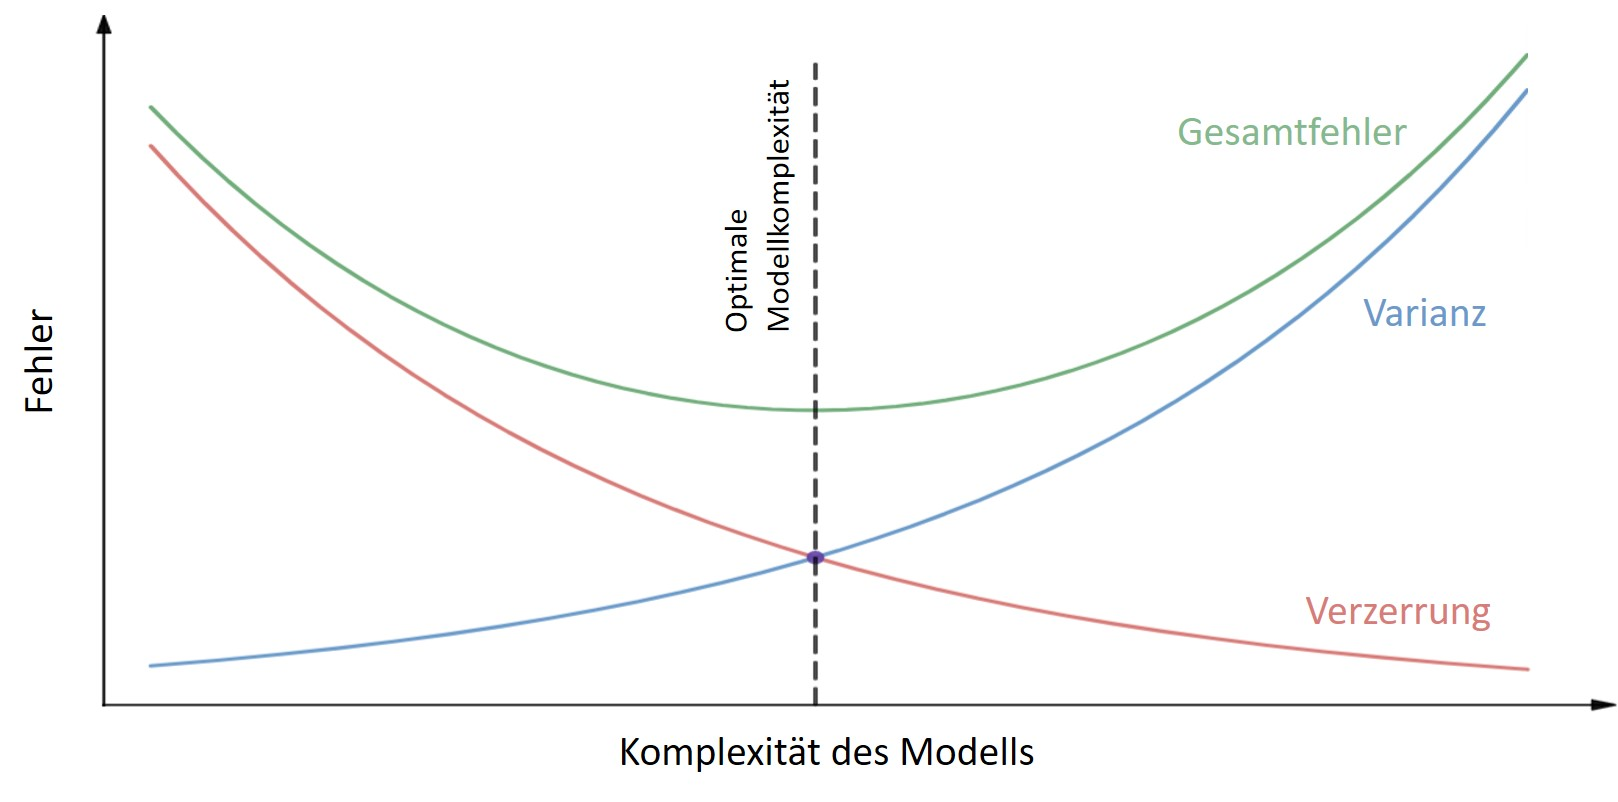
\includegraphics[width = 0.9\textwidth]{figures/bias_variance_tradeoff_labeled.jpg}
\caption{Verzerrung-Varianz-Dilemma}
\label{bias_variance_tradeoff}
\end{figure}

\subsection{Lineare Regression}

Bei der Regressionsanalyse werden Zusammenhänge zwischen
mehreren Merkmalen untersucht. Man versucht eine unabhängige Variable $Y$ durch eine oder mehrere abhängige Variablen $X_1, \ldots, X_p$ zu erklären. Ein lineares Regressionsmodell hat also die Form
\begin{align}
\label{linear_model}
f(X) = \beta_0 + \sum_{j=1}^p X_j\beta_j
\end{align}
wobei $\beta_j$ die Regressionskoeffizienten sind. Bei der Verwendung dieses Modells nehmen wir an, dass die Regressionsfunktion $\text{E}(Y|X)$ linear ist bzw. ein lineares Modell eine geeignete Approximation ist \cite{hastie_elements}.

Typischerweise verfügen wir über eine Menge von Trainingsdaten $(x_1, y_1), \ldots, (x_n, y_n)$. Jedes $x_i = (x_{i1}, \ldots, x_{ip})^{\top}$ stellt eine Beobachtung dar, die wir für die Schätzung der Parameter $\beta_j$ benutzen. Die bekannteste Methode für diesen Zweck ist sicherlich die \textit{Methode der kleinsten Quadraten} (Englisch: \textit{(Ordinary) Least Squares}), in welcher wir $\beta = (\beta_0, \ldots, \beta_p)^{\top}$ so wählen, dass die Summe der Residuenquadrate (Englisch: \textit{Residual Sum of Squares (RSS)} minimiert wird. Wir definieren
\begin{align}
\label{RSS}
\text{RSS}(\beta) & = \sum_{i=1}^{n}(y_i - f(x_i))^2\\
& = \sum_{i=1}^{n}(y_i - \beta_0 - \sum_{j=1}^p x_{ij}\beta_j)^2\nonumber\\
& = (y - \mat X \beta)^{\top}(y-\mat X \beta)\nonumber\\
& = \norm{y - \mat X \beta}_{2}^{2}\nonumber
\end{align}
und das dazugehörige Minimierungsproblem
\begin{align}
\label{least_squares}
\hat{\beta}^{\text{OLS}} = \argmin_{\beta} \text{RSS}(\beta)
\end{align}
wobei $\mat X \in \mathbb{R}^{n \times (p+1)}$ die Matrix der $x_i$ mit einer 1 an erster Stelle ist und $y = (y_1, \ldots, y_n)^{\top}$. An dieser Stelle möchten wir erwähnen, dass bei Verwendung dieser Methode keine Aussage über die Gültigkeit des Modells getroffen, sondern lediglich die beste lineare Approximation gefunden wird.

Falls $\mat X$ vollen Rang hat zeigt man leicht, dass (\ref{least_squares}) die eindeutige Lösung
\begin{align}
\hat{\beta}^{\text{OLS}} = (\mat X^{\top}\mat X)^{-1}\mat X^{\top} y
\end{align}
besitzt. Die Zielgröße $y$ ergibt sich dann durch
\begin{align}
\hat{y} = \mat X \hat{\beta}^{\text{OLS}} = \mat X (\mat X^{\top}\mat X)^{-1}\mat X^{\top} y
\end{align}
Die Matrix $\mat P = \mat X (\mat X^{\top}\mat X)^{-1}\mat X^{\top}$ haben wir bereits in Abschnitt \ref{orthogonality} kennengelernt. Sie projiziert $y$ orthogonal auf den durch die Spalten von $\mat X$ aufgespannten Unterraum. Dies ermöglicht eine geometrische Interpretation der linearen Regression.

Wenn $\mat X$ keinen vollen Rang hat, ist die Lösung von (\ref{least_squares}) nicht mehr eindeutig. Dieser Art Probleme ereignen sich häufig in der Bild- und Signalanalyse, bei welcher wir häufig über mehr Variablen als Beobachtungen verfügen. Um ein gewünschtes Verhalten der Regression zu gewährleisten, bestehen verschiedene Möglichkeiten der Filterung oder Regularisierung. In letzterem Fall versehen wir den Regressionsterm mit sog. \textit{Straftermen}, welche eine bedeutende Rolle in den folgenden Kapitel spielen werden. Wir möchten diese mithilfe der linearen Regression einführen. Die Effekte der Strafterme können aber auf andere verallgemeinerte lineare Modelle übertragen werden. 

Die von uns eingeführten Strafterme werden vor allem eine Schrumpfung der Regressionskoeffizienten verursachen. Daher möchten wir zunächst motivieren, in welchen Situationen eine derartige Regularisierung hilfreich sein kann.
\begin{itemize}
\item Vorhersagegenauigkeit: Besonders in $p > n$-Fällen neigt ein lineares Regressionsmodell häufig zu einer Überanpassung an die Trainingsdaten. Um die Vorhersagegenauigkeit für ungesehene Testdaten zu verbessern, kann eine Erhöhung des Bias im Sinne des Verzerrung-Varianz-Dilemmas sinnvoll sein. Dies können wir beispielsweise dadurch erreichen, dass wir die Regressionskoeffizienten verkleinern oder sogar auf 0 setzen.
\item Interpretation: Eine hohe Anzahl an Variablen, die in das Modell einfließen erschwert unzweifelhaft eine Interpretation. Daher kann es von Vorteil sein nur einen Teil der Variablen für das Modell auszuwählen. Optimalerweise selektiert man solche, die eine möglichst genaue Vorhersage ermöglichen.
\end{itemize}

Ein naheliegender Ansatz zur Lösung dieser Probleme wäre es zu versuchen, eine $k$-Teilmenge der Variablen zu finden, die eine minimale Summe der Residuenquadrate aufweist. In \cite{hastie_elements} werden verschiedene Methoden zur exakten und approximativen Berechnung dieser Teilmenge beschrieben. Nicht immer wird die Genauigkeit der Vorhersagen durch Verwendung dieses Ansatzes besser. Dies liegt vor allem daran, dass Variablen für das Modell entweder ausgewählt oder verworfen werden. Daher beschäftigen wir uns nun mit Methoden, die eine kontinuierliche Schrumpfung der Regressionskoeffizienten erlauben.\\

\subsection{Ridge Regression}

Zu diesem Zweck kann die \textit{Tikhonov Regularisierung}, die auch unter dem Namen \textit{Ridge Regression} bekannt ist, genutzt werden. Mithilfe eines \textit{Ridge Strafterms} opfern wir einen Teil des Bias für verbesserte Vorhersagen im Sinne des Verzerrung-Varianz-Dilemmas. Wir formulieren das Ridge Regression Problem in der Lagrange Form
\begin{align}
\label{ridge_regression}
\hat{\beta}^{\text{ridge}} = \argmin_{\beta} \sum_{i=1}^{n}(y_i - \beta_0 - \sum_{j=1}^p x_{ij}\beta_j)^2 + \lambda\sum_{j=1}^p \beta_j^2
\end{align}
wobei $\lambda \geq 0$ ein Parameter ist, der die Stärke der Schrumpfung der Regressionskoeffizienten kontrolliert. Je größer $\lambda$, desto stärker ist die Schrumpfung der $\beta_j$. Durch die Einführung des $ell_2$-Strafterms garantiert (\ref{ridge_regression}) auch für $p > n$ eine eindeutige Lösung. Da $\beta_0$ nicht im Strafterm vorkommt, schätzen wir zunächst $\beta_0 = \bar{y} = \frac{1}{n}\sum_{i=1}^{n} y_i$ und zentrieren die Eingaben $x_{ij} = x_{ij} - \bar{x}_j$. Die eindeutige Lösung der zentrierten Version von (\ref{ridge_regression}) ist dann durch
\begin{align}
\hat{\beta}^{\text{ridge}}  = (\mat X^{\top} \mat X + \lambda\mat{I})^{-1}\mat{X}^{\top}y
\end{align}
gegeben, wobei $\beta = (\beta_1, \ldots, \beta_p)$ und $\mat{X} \in \mathbb{R}^{n \times p}$ die Matrix der $x_i$. Die durch die Ridge Regression erzeugten Koeffizienten sind also um den Faktor $\frac{1}{1+\lambda}$ gegenüber denen der klassischen linearen Regression skaliert. Eine Dünnbesetzung der Koeffizienten wird also erst für $\lambda \to \infty$ erreicht.\\


\subsection{LASSO}
\label{lasso}

Um eine bessere Interpretation des Modells zu ermöglichen, versucht man bei der \textit{Lasso} Regression eine Lösung zu finden, bei welcher viele Koeffizienten gleich Null sind. Das Lasso wurde erstmals von Tibshirani in \cite{tibshirani_lasso} eingeführt und ist in der Signalanalyse unter dem Namen \textit{Basis Pursuit} \cite{chen} bekannt. Mathematisch gesehen erreichen wir eine Dünnbesetzung durch Einbettung eines $\ell_1$-Strafterms.
\begin{align}
\label{lasso_formulation}
\hat{\beta}^{\text{lasso}} = \argmin_{\beta} \sum_{i=1}^{n}(y_i - \beta_0 - \sum_{j=1}^p x_{ij}\beta_j)^2 + \lambda\sum_{j=1}^p \left|\beta_j\right|
\end{align}
Es wird also im Vergleich zu (\ref{ridge_regression}) lediglich die $\ell_2$-Norm durch eine $\ell_1$-Norm ausgetauscht. Bevor wir uns mit der Lösung dieses Problems beschäftigen, möchten wir erklären, warum die $\ell_1$-Norm eine Dünnbesetzung hervorruft. Zunächst geben wir eine geometrische Erklärung, welche in Abbildung \ref{lasso_ridge_regression_figure} zu sehen ist. Dort sind die $\ell_1$- und $\ell_2$-Beschränkungen, sowie die Höhenlinien der RSS-Funktion in zwei Dimensionen aufgezeichnet. Die optimalen Koeffizienten von Ridge und Lasso Regression ergeben sich nun aus dem Schnittpunkt der Höhenlinien mit der Begrenzung der jeweiligen Norm. Im Falle der $\ell_1$-Norm ist dieser Schnittpunkt mit einer hohen Wahrscheinlichkeit an eine der Ecken, so dass einer der beiden Koeffizienten auf Null gesetzt wird. Im Gegensatz dazu ist die Wahrscheinlichkeit, dass ein Koeffizient bei einer $\ell_2$-Begrenzung auf Null gesetzt wird, sehr gering, da keine Ecken vorhanden sind. Somit kommt jeder Randpunkt der Begrenzung als Schnittpunkt in Frage und es wird keine Dünnbesetzung, sondern lediglich eine kontinuierliche Schrumpfung der Koeffizienten hervorgerufen. Dieser Effekt verstärkt sich in höheren Dimensionen.

\begin{figure}
\centering
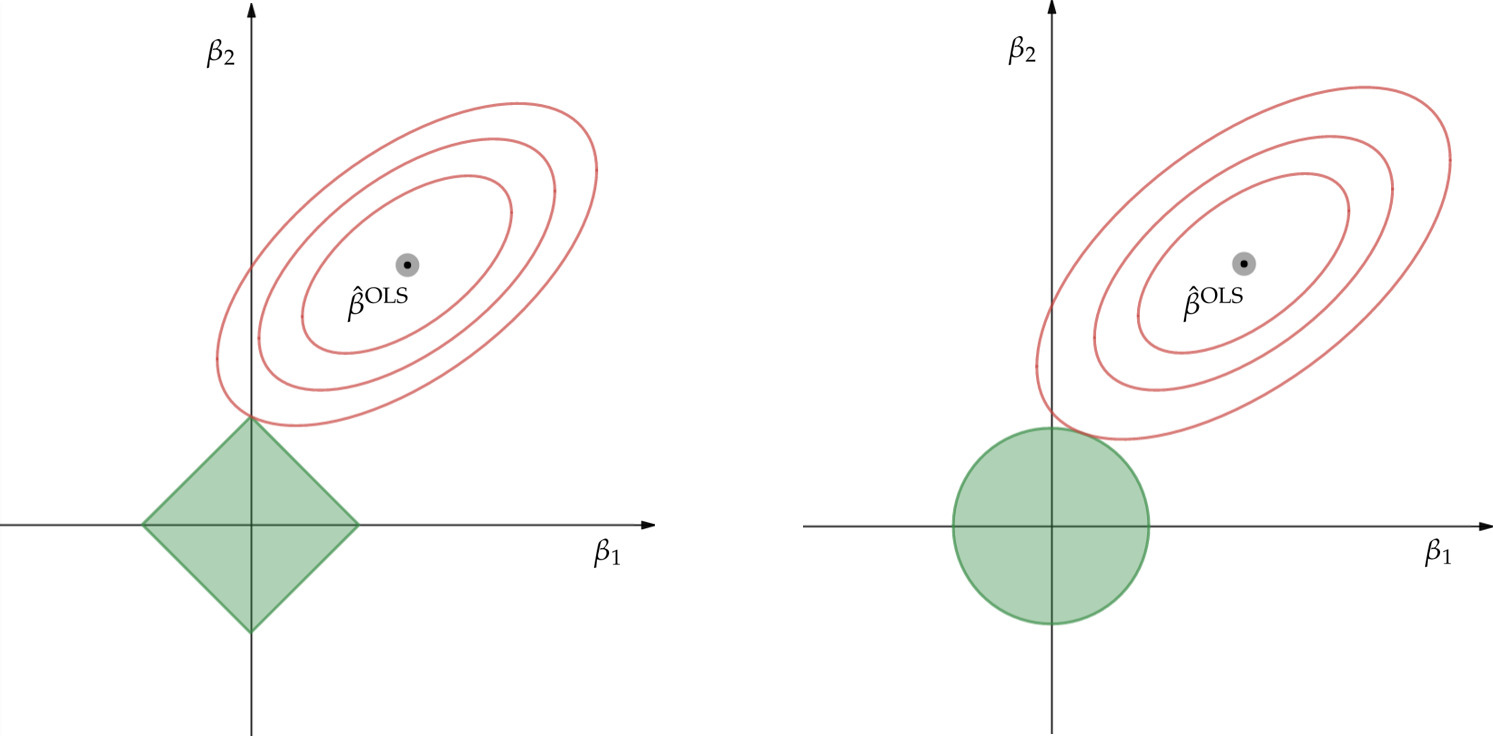
\includegraphics[width = 0.9\textwidth]{figures/lasso_ridge_regression.jpg}
\caption{Die Abbildung zeigt die Beschränkungen der $\ell_1$-Norm (links) und der $\ell_2$-Norm (rechts) zusammen mit den Höhenlinien der RSS-Funktion im $\mathbb{R}^2$. Verdeutlicht wird hier die geometrische Findung von $\hat{\beta}^{\text{lasso}}$ (links) und $\hat{\beta}^{\text{ridge}}$ (rechts). (Abbildung basiert auf \cite{hastie_elements})}
\label{lasso_ridge_regression_figure}
\end{figure}

An dieser Stelle kann man auf den Gedanken kommen, andere Strafterme zu verwenden, welche bei geometrischer Betrachtung die Wahrscheinlichkeit erhöhen eine Dünnbesetzung der Koeffizienten hervorzurufen. So kann man zum Beispiel die $\ell_q$-Normen als Strafterm für Werte $q < 1$ in Betracht ziehen. In Abbildung \ref{norm_figure} sind die Begrenzungen der $\ell_q$-Normen für verschiedene Werte von $q$ eingezeichnet. Für $q \rightarrow 0$ entstehen sternförmige Höhenlinien, welche immer weiter zum Ursprung gedrückt werden. Somit wird es immer wahrscheinlicher, dass die Höhenlinien der RSS-Funktion eine Ecke treffen und wir dünnbesetzte Koeffizienten erhalten. Daher kann man folgendes Berechnungsproblem definieren
\begin{align}
\label{sparse_regression}
\hat{\beta}^{\text{sparse}} = \argmin_{\beta} \sum_{i=1}^{n}(y_i - \beta_0 - \sum_{j=1}^p x_{ij}\beta_j)^2 + \lambda\sum_{j=1}^p \left|\beta_j\right|^q
\end{align}
Leider ist dies nur in der Theorie ein guter Ansatz. Das Problem liegt nicht im Effekt der verschiedenen Strafterme, sondern in der Berechnung. Für $q < 1$ ist (\ref{sparse_regression}) ein nicht-konvexes Optimierungsproblem, da $\norm{\cdot}_q$ keine Norm gemäß Definition \ref{norm} ist. Im Extremfall der $\ell_0$-\q{Norm} wird (\ref{sparse_regression}) sogar NP-schwer \cite{foucart}. Somit besteht keine effiziente Methode zur Berechnung von $\hat{\beta}^{\text{sparse}}$ zur Verfügung. Der Wert $q = 1$ ist eine Art Kompromisslösung, die einerseits effizient zu berechnen ist und andererseits noch immer eine dünnbesetzte Lösung liefert.

\begin{figure}
\centering
	\begin{subfigure}{0.2\textwidth}
	\centering
	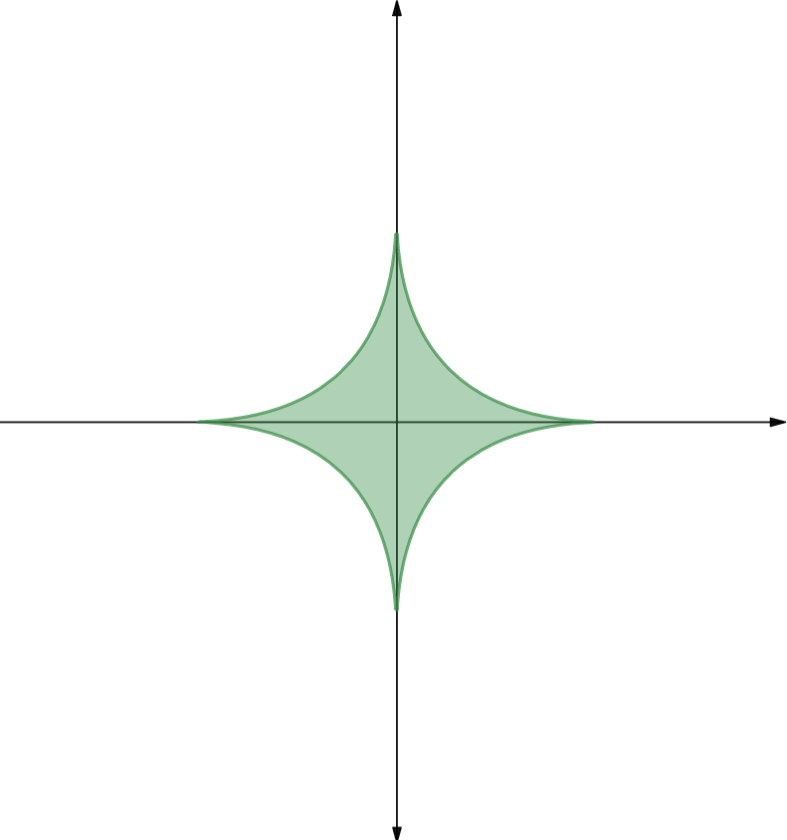
\includegraphics[width = \textwidth]{figures/norm_0_5.png}
	\label{norm_0_5_figure}
	\caption*{$q = 0.5$}
	\end{subfigure} \hspace{0.5cm}
	%	
	\begin{subfigure}{0.2\textwidth}
	\centering
	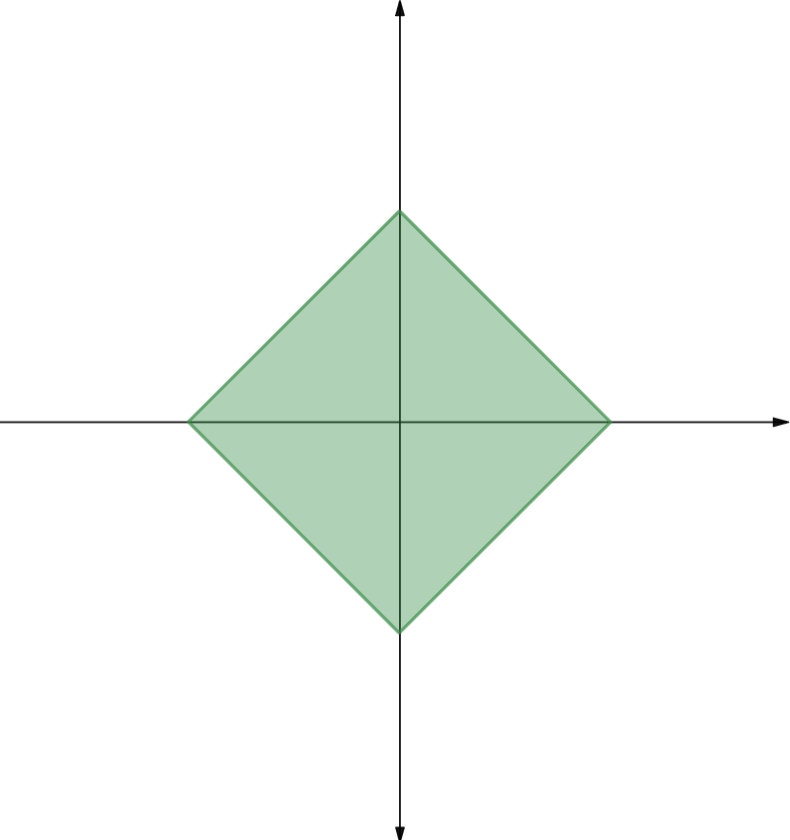
\includegraphics[width = \textwidth]{figures/norm_1.png}
	\label{norm_1_figure}
	\caption*{$q = 1$}
	\end{subfigure}\hspace{0.5cm}
	%
	\begin{subfigure}{0.2\textwidth}
	\centering
	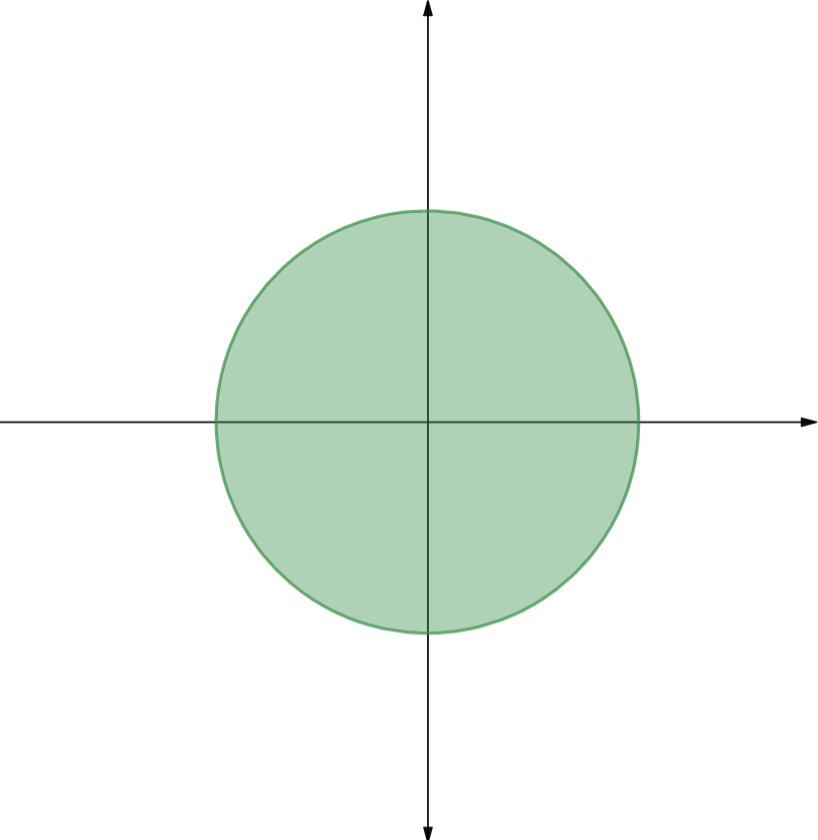
\includegraphics[width = \textwidth]{figures/norm_2.png}
	\label{norm_2_figure}
	\caption*{$q = 2$}
	\end{subfigure}\hspace{0.5cm}
	%
	\begin{subfigure}{0.2\textwidth}
	\centering
	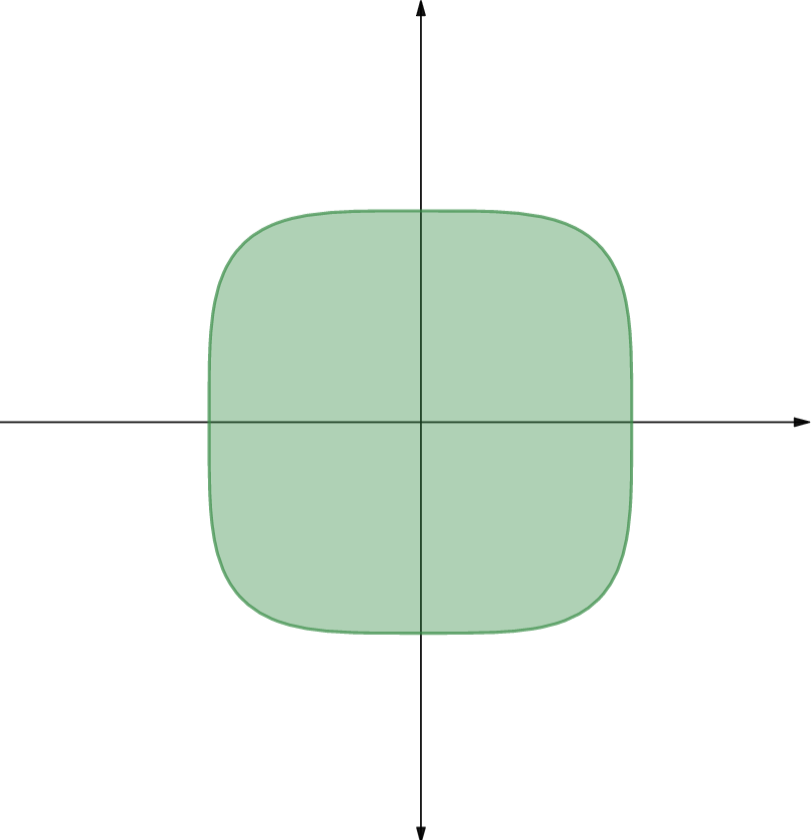
\includegraphics[width = \textwidth]{figures/norm_4.png}
	\label{norm_4_figure}
	\caption*{$q = 4$}
	\end{subfigure}

\caption{Die Abbildung zeigt die Begrenzungen der $\ell_q$-Norm im $\mathbb{R}^2$ für verschiedene Werte von $q$, also die Mengen $\{x \in \mathbb{R}^2 \colon \norm{x}_{q} \leq c \}$. (Abbildung basiert auf \cite{hastie_elements})}
\label{norm_figure}
\end{figure}

Um eine mathematisch gründliche Erklärung für die Dünnbesetzung zu liefern, wenden wir uns der Lösung von (\ref{lasso_formulation}) zu. Diese kann nur dann explizit angegeben werden, wenn $\mat X$ orthonormale Spalten hat. Es hilft uns aber trotzdem diese Lösung zu verstehen??
\begin{align}
\hat{\beta}_j^{\text{lasso}} = \text{sign}(\hat{\beta}_j^{\text{OLS}}) \left(\left|\hat{\beta}_j^{\text{OLS}}\right| - \frac{\lambda}{2}\right)_{+}
\end{align}
wobei $(\cdot)_+ = max(\cdot, 0)$ ist. Der Beweis kann in \cite{murphy} nachgelesen werden. Die Lösung ist also durch den der sog. \textit{soft thresholding operator} gegeben, welcher durch
\begin{align}
\text{soft}_{\delta}(x) = \text{sign}(x)(|x| - \delta)_+
\end{align}
definiert wird.

Der Operator ist in Abbildung \ref{thresholding_figure} noch einmal graphisch dargestellt. Nun sind wir auch in der Lage zu verstehen, warum Tibshirani \cite{tibshirani_lasso} den Begriff Lasso eingeführt hat. Dieser steht für \textit{Least absolute selection and shrinkage operator}, was bedeutet, dass ein Teil der Koeffizienten $\hat{\beta}_j^{\text{OLS}}$ ausgewählt und im Betrag geschrumpft wird. Die neuen Lasso Koeffizienten ergeben sich also dadurch, dass zunächst alle Koeffizienten in $\hat{\beta}^{\text{OLS}}$, die kleiner als $\frac{\lambda}{2}$ sind, auf $0$ gesetzt werden und anschließend die Verbliebenden im Betrag um $\frac{\lambda}{2}$ geschrumpft werden. Somit ist klar, dass für $\lambda \geq \lambda_{\text{max}}$ alle Koeffizienten $\hat{\beta}_j^{\text{lasso}} = 0$ sind, wobei $\lambda_{\text{max}} = \norm{\mat X^{\top}y}_{\infty}$. (Der Wert $\lambda_{\text{max}}$ beruht auf der Beobachtung, dass $0$ der optimale Wert der Koeffizienten ist falls $(\mat X^{\top}y)_j \in [-\lambda, \lambda]$ für alle $j$.) 

\begin{figure}
\centering
	\begin{subfigure}{0.4\textwidth}
	\centering
	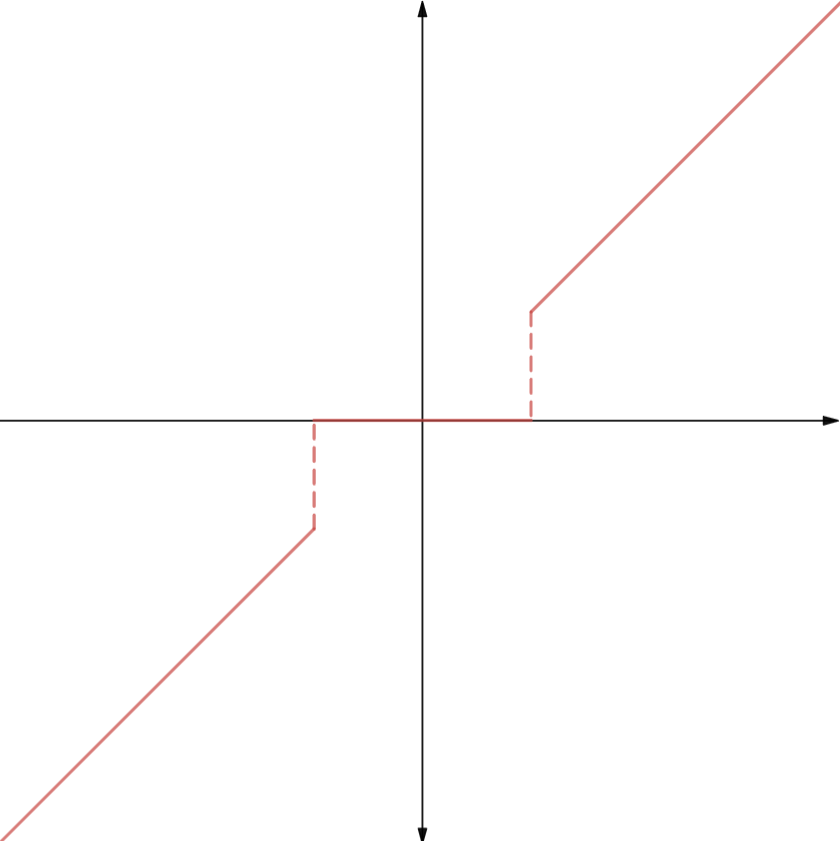
\includegraphics[width = \textwidth]{figures/hard_thresholding.png}
	\label{hard_thresholding}
	\end{subfigure}\hspace{1cm}
	%	
	\begin{subfigure}{0.4\textwidth}
	\centering
	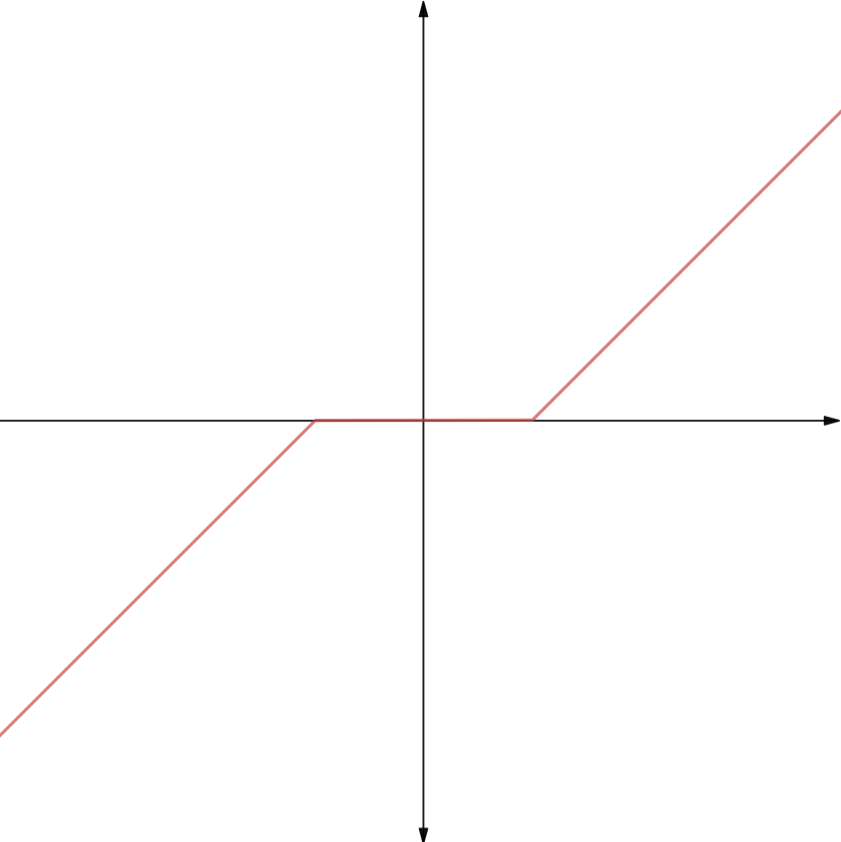
\includegraphics[width = \textwidth]{figures/soft_thresholding.png}
	\label{soft_thresholding}
	\end{subfigure}
\caption{Die Abbildung zeigt die beiden Operationen soft und hard thresholding}
\label{thresholding_figure}
\end{figure}

Wir wenden uns nun einer mathematischen Lösung des Lasso zu. Im Gegensatz zu Ridge Regression kann man im Allgemeinen keine explizite Lösung angeben. Nur für den Fall, dass.
Da $\norm{\beta}_1$ nicht differenzierbar ist wenn $\beta_j = 0$ ist, sind wir bei (\ref{lasso_formulation}) mit einem nicht glattem Optimierungsproblem konfrontiert. Seit der Problemformulierung in 1996 wurde eine Vielzahl an Algorithmen entwickelt bzw. adaptiert, die eine numerische Lösung liefern. Dazu gehören Least-angle Regression (LARS) \cite{efron_lars}, Koordinaten-Abstiegsverfahren \cite{friedman}, Subdifferential Methoden und  Näherungs-Gradientenverfahren \cite{yang, vandenberghe}. Letztere sind eine natürliche Erweiterung von Gradientenverfahren wenn die Zielfunktion nicht differenzierbar ist. Wir werden später auf das Koordinaten-Abstiegsverfahren näher eingehen, welches wir bei der Implementierung der dünnbesetzten Hauptkomponentenanalyse nutzen.

Es stellt sich heraus, dass das Lasso zwei wesentliche Nachteile besitzt. Falls es im Datensatz Gruppen stark korrelierter Variablen gibt, so tendiert die Methode dazu nur eine Variable aus einer Gruppe statt die Gruppe als Ganzes auszuwählen. In vielen Anwendungen ist man aber gerade daran interessiert. Zum Beispiel bei der Suche nach Genen, welche mit einer bestimmten Krankheit verbunden sind, möchte man alle assoziierten Koeffizienten finden anstatt nur einem Gen aus einer Gruppe. Darüber hinaus führt dies oft dazu, dass der Vorhersagefehler vergrößert wird und somit die Methode nicht ganz so robust ist. Um diesem Problem zu entgegnen kann man das sog. \textit{Group Lasso} verwenden \cite{yuan}, bei welcher man zuvor Gruppen im Datensatz festlegen kann. Der im Zuge dieser Arbeit aber wichtigere Aspekt ist, dass das Lasso im Fall $p > n$ maximal $n$ Variablen selektieren kann. Dies ist für moderne Datensätze, für welche $p \gg n$ gilt oft nicht ausreichend. Der Grund dafür wird in ... klar. Why LASSO can select at most n predictors https://stats.stackexchange.com/questions/386116/why-does-lasso-select-at-most-n-predictors\\

\subsection{Elastic Net}

Damit im Fall $p > n$ mehr als $n$ Variablen selektiert werden, kann man die beiden vorgestellten Methoden kombinieren. Durch die Einbettung einer $\ell_1$ und $\ell_2$-Norm erhalten wir das sog. \textit{Elastic Net} \cite{zou_elasticnet}.
\begin{align}
\label{elastic_net}
\hat{\beta}^{\text{en}} = \argmin_{\beta} \norm{y - \mat X \beta}_2^2 + \lambda_2 \norm{\beta}_{2}^{2} + \lambda_{1,j} \norm{\beta}_{1}
\end{align}
Wie zuvor wird durch den $\ell_1$-Strafterm ein dünnbesetztes Modell generiert. Der $\ell_2$-Strafterm fördert den Gruppeneffekt, stabilisiert den $\ell_1$ Regularisierungspfad und lässt eine beliebige Anzahl zu selektierender Variablen zu.

Ähnlich wie bei der Lasso Regression kann nur im Fall orthogonaler Spalten von $\mat X$ eine explizite Lösung mithilfe des soft thresholding operators von (\ref{elastic_net}) angegeben werden. Mit leichten Modifikationen der Algorithmen für das Lasso erhalten wir eine numerische Lösung. So wurde LARS-EN \cite{zou_elasticnet} oder ein Koordinatenabstiegsverfahren vorgeschlagen \cite{friedman}.

We propose an efficient algorithm called LARS-EN to solve the elastic net efficiently, which is
based on the recently proposed algorithmLARSof Efron et al. (2004). They proved that, starting
from zero, the lasso solution paths grow piecewise linearly in a predictable way. They proposed
a new algorithm called LARS to solve the entire lasso solution path efficiently by using the same
order of computations as a single OLS fit\\

\subsection{Vergleich der Regressionsmethoden}
\label{comparison_linear_models}

Zur Veranschaulichung der oben eingeführten Methoden werden wir diese auf ein Beispiel anwenden. Dabei greifen wir auf einen durch scikit-learn \cite{scikit_learn} bereitgestellten Datensatz, der erstmals durch \cite{efron_lars} öffentlich gemacht worden ist, zurück. In diesem wurden für $n = 442$ Diabetes Patienten $p=10$ verschiedene Variablen gemessen. Dazu gehören Alter (AGE), Geschlecht (SEX), Body Mass Index (BMI), Blutdruck (BP) und verschiedene Blutproben (Serum Measurements). Die Zielgröße $y$ enthält Werte für den Krankheitsfortschritt ein Jahr nach Behandlungsbeginn. Ein Ausschnitt des Datensatzes befindet sich in Tabelle \ref{diabetes_data_set}.

\begin{table}
\centering
\begin{tabular}[c]{c|cccccccccc|c}
& \thead{AGE} & \thead{SEX} & \thead{BMI} & \thead{BP} & \multicolumn{6}{c|}{\ldots \thead{Serum Measurements} \ldots} & \thead{Response}\\
\thead{Patient} & \thead{x1} & \thead{x2} & \thead{x3} & \thead{x4} & \thead{x5} & \thead{x6} & \thead{x7} & \thead{x8} & \thead{x9} & \thead{x10} & \thead{y}\\
\hline
1 & 59 & 2 & 32.1 & 101 & 157 & 93.2 & 38 & 4 & 4.9 & 87 & 151\\
2 & 48 & 1 & 21.6 & 87 & 183 & 103.2 & 70 & 3 & 3.9 & 69 & 75\\
3 & 72 & 2 & 30.5 & 93 & 156 & 93.6 & 41 & 4 & 4.7 & 85 & 141\\
4 & 24 & 1 & 25.3 & 84 & 198 & 131.4 & 40 & 5 & 4.9 & 89 & 206\\
\vdots & \vdots & \vdots & \vdots & \vdots & \vdots & \vdots & \vdots & \vdots & \vdots & \vdots & \vdots\\
441 & 36 & 1 & 30.0 & 95 & 201 & 125.2 & 42 & 5 & 5.1 & 85 & 220\\
442 & 36 & 1 & 19.6 & 71 & 250 & 133.2 & 97 & 3 & 4.6 & 92 & 57\\
\end{tabular}
\caption{Diabetes Datensatz \cite{efron_lars, diabetes_data}}
\label{diabetes_data_set}
\end{table}

Schrumpfung bei Ridge Regression kontinuierlich.
Die Ergebnisse der Regressionen können in Abbildung \ref{regression_coefficients} und \ref{regression_coefficients_mse} eingesehen werden. 

Die Implementierung des Elastic Nets in scikit-learn \cite{scikit_learn} beruht auf einer anderen, aber sehr ähnlichen mathematischen Formulierung
\begin{align}
\label{elastic_net_python}
\hat{\beta}^{\text{en}} = \argmin_{\beta} \frac{1}{2n} \norm{y - \mat X \beta}_2^2 + \alpha \gamma \norm{\beta}_{2}^{2} + \frac{1}{2}\alpha (1-\gamma) \norm{\beta}_{1}
\end{align}
wobei $n$ die Anzahl an Beobachtungen im Datensatz und $\gamma$ das Verhältnis der $\ell_2$- zur $\ell_1$-Norm ist. Wählen wir $\gamma = 0$ so reduziert sich (\ref{elastic_net_python}) auf Ridge Regression und für $\gamma = 1$ auf das Lasso. So können wir mit $\gamma$ das Verhältnis der beiden Regressionen kontrollieren und mit $\alpha$ die Stärke der Bestrafung. Man beachte, dass bei dieser Implementierung nicht die Möglichkeit besteht die Koeffizienten unterschiedlich zu bestrafen.
Setzt man 
\begin{align}
 \alpha = \frac{2\lambda_2 + \lambda_1}{2n} \quad \text{und} \quad \gamma = \frac{\lambda_1}{2\lambda_2 + \lambda_1}
\end{align}
so reduziert sich (\ref{elastic_net_python}) auf unser ursprünglich formuliertes Problem.

\begin{figure}
\centering
	\begin{subfigure}{0.9\textwidth}
	\centering
	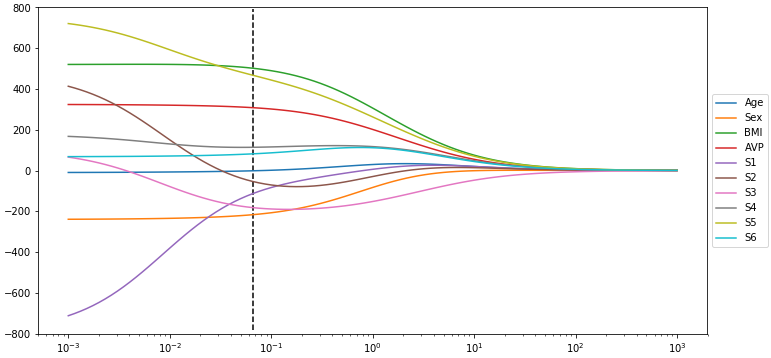
\includegraphics[width = \textwidth]{figures/ridge_regression_coefficients_cv.png}
	\label{ridge_regression_coefficients}
	\vspace{-0.5cm}
	\caption{Ridge Regression}
	\vspace{0.5cm}
	\end{subfigure}
	%	
	\begin{subfigure}{0.9\textwidth}
	\centering
	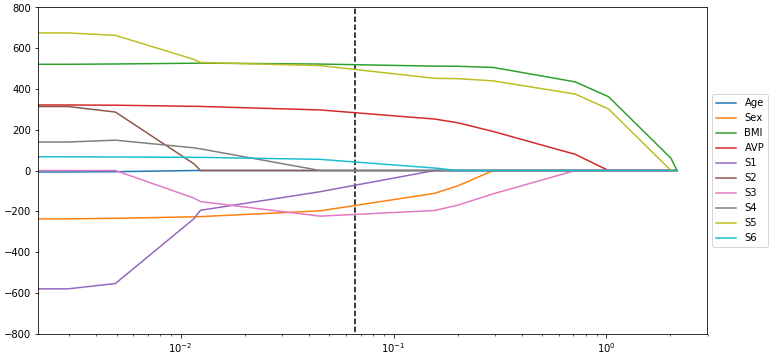
\includegraphics[width = \textwidth]{figures/lasso_regression_coefficients_cv.png}
	\label{lasso_regression_coefficients}
	\vspace{-0.5cm}
	\caption{Lasso Regression}
	\vspace{0.5cm}
	\end{subfigure}
	%
	\begin{subfigure}{0.9\textwidth}
	\centering
	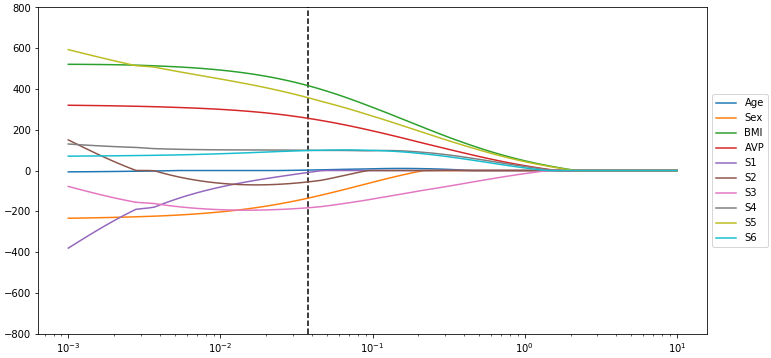
\includegraphics[width = \textwidth]{figures/elastic_net_coefficients_cv.png}
	\label{elastic_net_coefficients}
	\vspace{-0.5cm}
	\caption{Elastic Net, $\gamma = 0.98$}
	\end{subfigure}
\caption{Schrumpfung der Koeffizienten für verschiedene Regressionsmethoden bei Erhöhung des jeweiligen Regularisierungsparameters. Die vertikalen Linien stellen den Wert des jeweiligen Parameters dar, der durch ein 10-faches Kreuzvalidierungsverfahren bestimmt worden ist. (Erstellt mit scikit-learn)}
\label{regression_coefficients}
\end{figure}

\begin{figure}
\centering
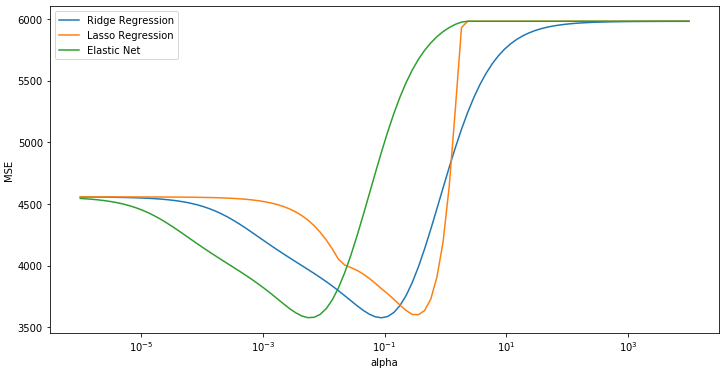
\includegraphics[width=0.9\textwidth]{figures/regression_coefficients_mse.png}
\label{regression_coefficients_mse}
\caption{Selektion des Modells gemäß der mittleren quadratischen Abweichung für Ridge, Lasso und Elastic Net Regression}
\end{figure}


%----------------------------------------------------------------------------------------
%	Signaltheorie
%----------------------------------------------------------------------------------------


\section{Signaltheorie}
\label{signal_processing}

\subsection{Fouriertransformation}
\subsection{Nyquist-Shannon Abtasttheorem}
% Main chapter title
\chapter{Hauptkomponentenanalyse}

% Chapter label
\label{pca}

To Do: Kovarianzmatrix / Stichprobenkovarianzmatrix einheitlich!
Begriffe wie samples, PCA, oder features erklären, EIGENVALUE = VARIANCE

Die Hauptkomponentenanalyse ist ein weitverbreitetes multivariates statistisches Verfahren zur Dimensionsreduktion. Multivariate Verfahren zielen darauf ab, die in einem Datensatz enthaltene Zahl der Variablen zu verringern, ohne die darin enthaltene Information (zu verlieren) / (wesentlich zu reduzieren). Dadurch können umfangreiche Datensätze strukturiert, veranschaulicht und vereinfacht werden. Somit ist das Verfahren Teil der explorativen Statistik, welche Datensätze hinsichtlich ihrer Zusammenhänge analysiert. Die sich ergebende Struktur kann für weitere Analysezwecke ausgenutzt werden.

Aus diesem Grund hat die Hauptkomponentenanalyse in vielen Bereichen erfolgreich Anwendung gefunden. Darunter fällt die Erkennung handgeschriebener Zahlen, welche zum Beispiel zur automatischen Sortierung von Briefen nach Postleitzahl genutzt wird \cite{hastie_elements}. An diesem Beispiel lässt es sich besonders gut verdeutlichen, was es heißt Zusammenhänge zu analysieren und Strukturen auf den Daten zu finden. Man erhofft, dass nach Anwendung einer Dimensionsreduktion wie PCA auf den Datensatz 10 verschiedene Gruppierungen zu erkennen sind, die für die Ziffern 0 bis 9 stehen (siehe dazu Bild?). Optimalerweise gehören alle Datenpunkte im demselbem Cluster zur selben Ziffer. Außerdem korrespondieren nahe beieinanderliegende Cluster mit Ziffern, die ähnlich aussehen. Weitere Anwendung findet das Verfahren in der Bildverarbeitung. Hier kann es zum Beispiel zur Rauschunterdrückung \cite{babu} oder zur Gesichtserkennung \cite{jiang} genutzt werden. Um Bilder für solch ein Verfahren nutzbar zu machen, werden einzelne Pixel oder patches, also lokale Gruppierungen von Pixeln, eines Bildes als Variable interpretiert.

Das mathematische Problem der Hauptkomponentenanalyse kann auf verschiedene Weisen beschrieben werden. Zunächst wollen wir es so konstruieren, dass die Idee des minimalen Informationsverlust im Vordergrund steht. Anschließend werden wir das Problem auf eine Singulärwertzerlegung zurückführen, die auch zur effizienten Implementierung genutzt wird. Des Weiteren werden wir die Hauptkomponentenanalyse als Regressionsproblem betrachten und die geometrische Interpretation weiter verdeutlichen. Zu Schluss werden wir einige theoretische Aussagen angeben, die für die folgenden Kapitel relevant sind.

\section{Konstruktion}

Gegeben sei ein Datensatz mit $n$ samples und $p$ Variablen. Die zentrale Idee der Hauptkomponentenanalyse besteht darin, die $p$ bestehenden Variablen in $k$ neue, unkorrelierte Variablen zu überführen. Um eine Reduktion der Dimension, also $k < p$ zu erreichen, müssen die bestehenden Variablen \textit{zusammengefasst} werden. Idealerweise sollte bei diesem Prozess möglichst wenig Information verloren gehen. Als Maß für den Informationsgehalt der Daten wird hierbei die Varianz verwendet. Das heißt, je größer die Varianz einer Variable, desto mehr Information birgt sie und desto \textit{wichtiger} ist sie. Denn eine Variable, die für alle Beobachtungen ähnliche Werte aufweist, ist nicht von Nutzen bei der Unterscheidung verschiedener samples. Um die Dimension zu reduzieren könnte man einfach nach den Eigenschaften größter Varianz suchen und alle Variablen unterhalb eines festgelegten Grenzwertes verwerfen. Dieses Vorgehen fällt allgemein unter die Methodik der \textit{feature selection}. Die Hauptkomponentenanalyse verwendet allerdings ein anderes Prinzip, welches der Methodik der \textit{feature extraction} zuzuordnen ist: Anstatt Eigenschaften mit hoher Varianz auszuwählen, konstruiert man neue Variablen, die die Bestehenden zusammenfassen. Variablen mit hoher Varianz werden in der Konstruktion einen größeren Beitrag spielen.

Konkret suchen wir also sukzessive nach einer Linearkombination der bestehenden Variablen. Finden wir nun zunächst die Richtung größter Varianz in unserem Datensatz, die erste \textit{Hauptachse}. Der zugehörige Vektor spiegelt dabei den Beitrag bzw. den Informationsgehalt jeder einzelnen Variable wider. Anschließend finden wir weitere Hauptachsen, indem wir unter den Richtungen, die orthogonal zu allen vorherigen Hauptachsen sind, die mit der größten Varianz wählen. (Man iteriert diesen Prozess solange ...) Die Orthogonalität garantiert, dass die entstehenden Variablen unkorreliert sind. (Was hat das für einen Vorteil?) Nach der Identifizierung der Hauptachsen wollen wir unsere Beobachtungen bezüglich dieser darstellen. Wir erhalten die \textit{Hauptkomponenten} unseres Datensatzes, indem wir die einzelnen samples auf die Hauptachsen transformieren. Aufgrund der schrittweisen Konstruktion verfügen Diese über eine sehr wichtige Sortierung. So beinhaltet die erste Hauptkomponente die meiste Information. Mit jeder weiteren Hauptkomponente erhält man mehr Information, aber der Informationsgewinn wird mit jeder Hauptkomponente geringer. Abbildung SCREE PLOT verdeutlicht diesen Verlauf.

Die eigentliche Dimensionsreduktion findet dann durch Selektion statt. Je nach Komplexität des Modells, welches man erreichen möchte, können so mehr oder weniger Hauptkomponenten ausgewählt werden. Je mehr Hauptkomponenten man auswählt, desto mehr Information erhält man über den Datensatz. Allerdings wird das Modell mit steigender Anzahl an Variablen immer komplizierter. Es gilt einen Punkt der Balance zu finden, der ein gutes Mittel aus Information und Komplexität liefert. Dieser kann vom Anwendungsfall abhängen. Wir werden uns mit diesem Thema weiter in \ref{selection_principal_components} beschäftigen.
Zusammenfassend haben wir somit unseren ursprünglichen Datensatz in neuen Hauptkomponenten konzentriert, die aber trotzdem einen Großteil an Information beinhalten.

Um dieses Prinzip zu veranschaulichen, wenden wir uns nun einem simplem Beispiel zu. Gegeben seien die Größe [cm] und das Gewicht [kg] zu 1000 Personen (Daten sind simuliert, keine real-world-data) (siehe dazu Abbildung). In diesem Fall ist also $n = 1000$ und $p = 2$. Bei Betrachtung der Abbildung fällt schnell auf, dass die beiden Variablen positiv korreliert sind, d.h. prinzipiell erkennt man folgende Tendenz: Je größer eine Person, desto schwerer ist sie. 

\begin{figure}
\centering
	\begin{subfigure}{0.45\textwidth}
	\centering
	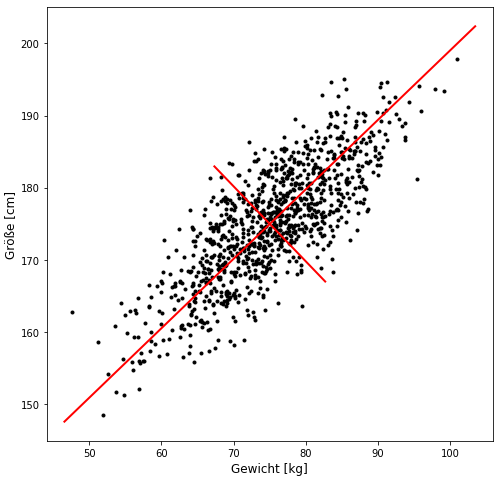
\includegraphics[width = \textwidth]{figures/pca_example.png}
	\label{pca_example_original}
	\end{subfigure}
	%	
	\begin{subfigure}{0.45\textwidth}
	\centering
	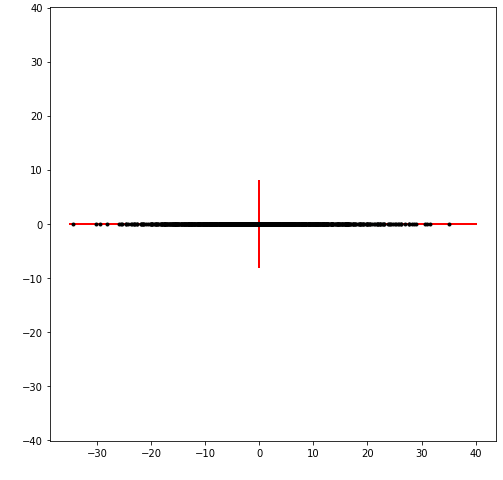
\includegraphics[width = \textwidth]{figures/pca_example_rotated.png}
	\label{pca_example_rotated}
	\end{subfigure}

\caption{Die Abbildung zeigt die Richtung größter Varianz ...}
\label{pca_example}
\end{figure}



\textbf{Standardisierung}

Bevor wir die Hauptkomponentenanalyse auf den Datensatz anwenden, gibt es aber noch einen wichtigen Bearbeitungsschritt zu beachten. Wenn eine Variable weniger variiert als eine Andere aufgrund der verwendeten Einheit oder Skala (meter oder kilo) kann dies zu ungewollten Ergebnissen führen. Ohne eine Vorbehandlung der Daten hat so im obigen Beispiel eine Änderung von 1m die gleiche Bedeutung wie eine Änderung von 1kg. (Satz schöner formulieren) Allerdings sind zwei Menschen, deren Größe 1m variiert, sehr verschieden, während zwei Menschen, die eine Differenz von 1kg haben, sehr ähnlich sind. Daher werden die Daten häufig einem sogenanntem preprocessing unterzogen. Ein zu diesem Zweck oft verwendetes Verfahren ist die Standardisierung oder auch z-Transformation genannt. In diesem Schritt werden die Variablen so transformiert, dass sie \textit{vergleichbarer} werden. Seien dazu $Y_i$ die Zufallsvariablen mit Erwartungswert $E[Y_i] = \mu$ und Varianz $Var[Y_i] = \sigma^2$. So erhält man die zugehörigen standardisierten Zufallsvariablen $X_i$ durch Zentrierung und anschließender Division durch die Standardabweichung $X_i = \frac{Y_i - \mu}{\sigma}$. Somit gilt dann:
\begin{itemize}
\item $E[X_i] = 0$ für alle $1 \leq i \leq p$
\item $Var[X_i] = 1$ für alle $1 \leq i \leq p$
\end{itemize}

Mathematisch gesehen wendet man das Verfahren also nicht auf die Kovarianzmatrix, sondern auf die Korrelationsmatrix an.

\subsection{Problemformulierung als Varianzmaximierung}

Wir wollen nun die Intuition des minimalen Informationsverlust mathematisch beschreiben. Gegeben sei dazu eine Matrix $\mat{X} \in \mathbb{R}^{n\times p}$, wobei $n$ die Anzahl der Samples bzw. Beobachtungen und $p$ die Anzahl der Variablen ist. Wir nehmen im Folgenden ohne Beschränkung der Allgemeinheit an, dass die Variablen zuvor zentriert wurden. Aufgabe der Hauptkomponentenanalyse ist es nun sukzessive Richtungen größter Varianz zu finden. Die erste Hauptkomponente ist definiert durch $Z_1 = \sum_{j=1}^p v_{1j}X_j = \mat{X}v$ wobei die Hauptachse $v_1 = (v_{11}, \ldots, v_{1p})^T$ so gewählt wird, dass die Varianz von $Z_1$ maximiert wird, d.h.
$$v_1 = \argmax_{\norm{v}_2 = 1} \text{Var}[\mat{X}v] = \argmax_{\norm{v}_2 = 1} v^T \mat{K}_{xx} v$$
mit $\mat{K_{xx}} = \frac{\mat{X}^T\mat{X}}{n-1}$ als Stichprobenkovarianzmatrix. Die restlichen Hauptachsen können nun sukzessive definiert werden.
$$v_{k+1} = \argmax_{\norm{v} = 1} v^T \mat{K}_{xx} v$$ 
$$v_{k+1}^Tv_l = 0 \quad \forall 1 \leq l \leq k$$
Man sucht also unter den Richtungen, die orthogonal zu allen bisherigen Hauptachsen sind, diejenige, die die Varianz maximiert. Wie oben beschrieben erhält man dann die Hauptkomponenten, also die Darstellung der Daten bezüglich der neu gefundenen Hauptachsen, durch Projektion der Daten $Z_i = \mat{X}v_i$.
\cite{zou_overview}
CITE JOLLIFE

Wie wir bereits in THEOREM gesehen haben, entsprechen die Eigenvektoren der Kovarianzmatrix genau den Richtungen maximaler Varianz. Daher können wir anstatt sukzessiver Berechnung einzelner Hauptachsen die Kovarianzmatrix $\mat{K}_{xx}$ direkt diagonalisieren. Dies ist möglich, da $\mat{K}_{xx}$ symmetrisch ist. Die Diagonalisierung ergibt
$$\mat{K}_{xx} = \mat V \mat L \mat{V}^T$$
wobei $\mat{L}$ eine Diagonalmatrix mit Eigenwerten $\lambda_i$ und $\mat V$ die Matrix der Eigenvektoren ist, d.h. jede Spalte entspricht einem Eigenvektor von $\mat{K}_{xx}$. Somit können die Hauptachsen direkt aus $\mat V$ abgelesen werden. Die Projektion der Daten auf die Hauptachsen wird dann wie zuvor durch Multiplikation der Beobachtungen mit den Eigenvektoren erreicht. 
$$\mat Z = \mat X \mat V$$
Die i-te Spalte in $\mat{Z}$ entspricht also der i-ten Hauptkomponente und die einzelnen Beobachtungen bezüglich der neuen Darstellung sind die Zeilen von $\mat{Z}$.


\subsection{Formulierung als Singulärwertzerlegung}
Es gibt einen engen Zusammenhang zwischen der Diagonalisierung der Kovarianzmatrix $\mat{K}_{xx} = \mat X^T \mat X$ und der Singulärwertzerlegung von $\mat X$. Diese Beziehung können wir nutzen, um das Problem neu zu formulieren. Eine Singulärwertzerlegung der Matrix $\mat X$ ergibt
$$ \mat{X} = \mat{U}\mat{D}\mat{V}^T $$
wobei $\mat{D}$ eine Diagonalmatrix mit Singulärwerten $d_1,\ldots,d_p$, $\mat{U}$ eine orthogonale $n \times p$ und $\mat{V}$ eine orthogonale $p \times p$ Matrix ist. Nun sieht man aufgrund der Orthogonalität von $\mat U$, dass
$$\mat{K}_{xx} = \mat X^T \mat X = \mat{V}\mat{D}\mat{U}^T \mat{U}\mat{D}\mat{V}^T = \mat V \mat{D}^2 \mat V^T$$
Wegen der Eindeutigkeit der Diagonalisierung(stimmt das?) ist $\mat V$ nun wie zuvor die Matrix der Eigenvektoren und somit der Hauptachsen. Ebenso stehen die Singulärwerte durch 
$$\lambda_i = \frac{d_i^2}{n-1}$$
in Beziehung mit den Eigenwerten der Kovarianzmatrix. Die Hauptkomponenten kann man somit auch durch $\mat X \mat V = \mat U \mat D$ erhalten.

Computing PCA using Eigen value decomposition of the sample covariance matrix:
We first have to compute the covariance matrix, which is $O(p^2n)$ and then compute its eigenvalue decomposition which is $O(p^3)$ giving a total cost of $O(p^2n+p^3)$ (https://arxiv.org/pdf/1503.05214.pdf)

Computing PCA using SVD of the data matrix:
Svd has a computational cost of $O(p^2n)$

Numerical Stability? Which method is preferrable in the $n << p$ case?


\subsection{Formulierung als beste Rang k Rekonstruktion}
Further multiplying the first k PCs by the corresponding principal axes $\mat V^T k$ yields $\mat X_k = \mat U_k \mat S_k \mat{V}_k^T$ matrix that has the original $n \times p$ size but is of lower rank (of rank k). This matrix $\mat X_k$ provides a reconstruction of the original data from the first k PCs. It has the lowest possible reconstruction error


\subsection{Formulierung als Regressionsproblem}

\begin{figure}
\centering
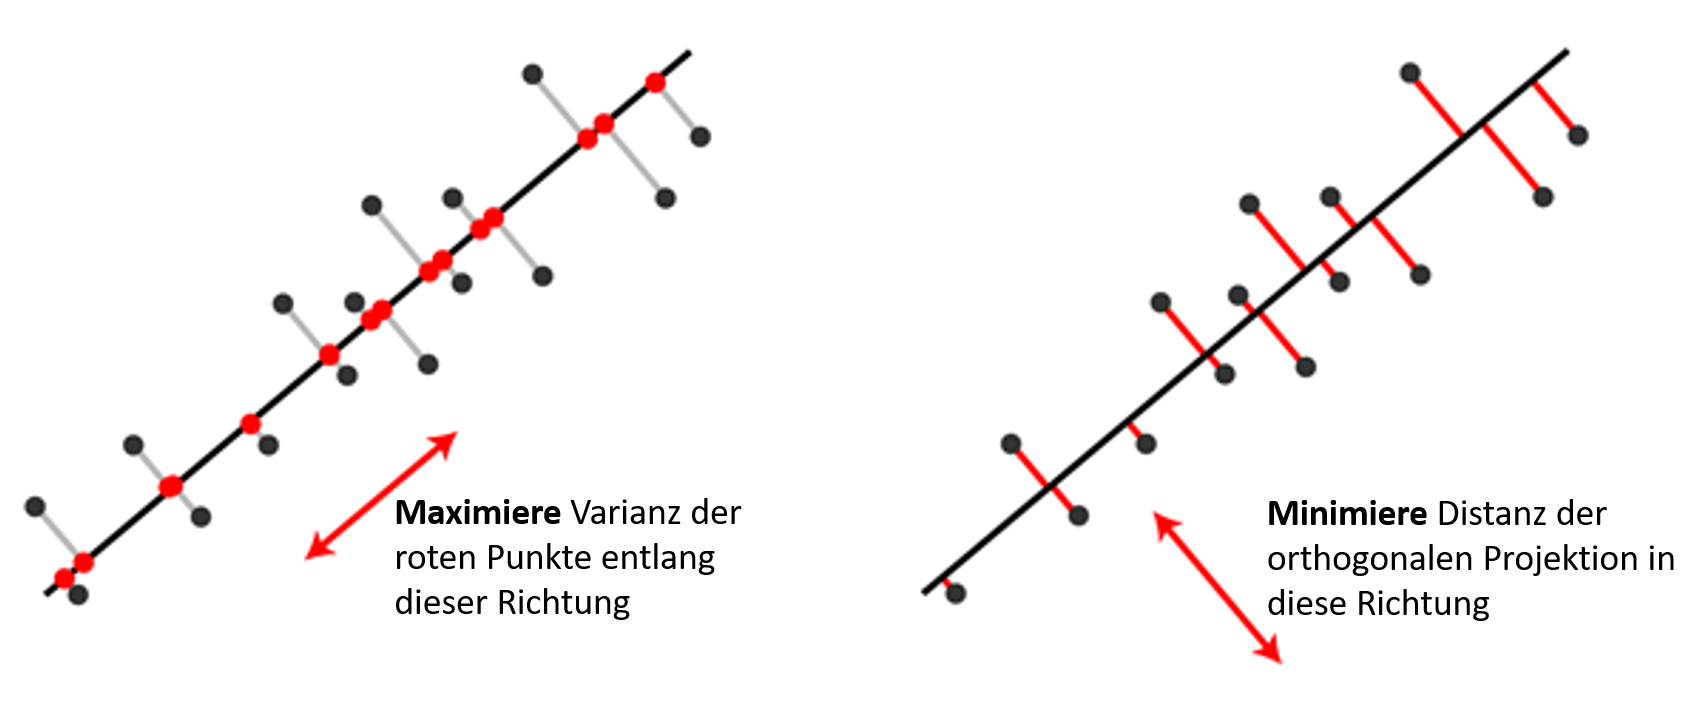
\includegraphics[width = 0.8\textwidth]{figures/pca_projection_explanation_german.png}
\caption{Die Abbildung zeigt die Äquivalenz von Maximierung der Varianz und Minimierung der Distanz der orthogonalen Projektion}
\label{pca_projection_explanation}
\end{figure}

Wir widmen uns nun einer letzten Formulierung der Hauptkomponentenanalyse, die eine geometrische Interpretation ermöglicht. Hierbei versucht man einen $k$-dimensionalen $(k < n)$ Unterraum zu finden, der die Daten bestmöglich approximiert. Wir werden diese Problemstellung nun mathematisch formulieren.

Sei dazu $x_i$ die i-te Beobachtung, also die i-te Zeile von $\mat X$ und $\mat V_k = \left[ V_1 \vert \cdots \vert V_k \right]$ eine $p \times k$ orthonormale Matrix. Nun projizieren wir jede Beobachtung orthogonal auf den durch $V_1, \ldots V_k$ aufgespannten Unterraum. Die orthogonale Projektion wird wie in REF beschrieben durch Multiplikation mit dem Operator $\mat V_k \mat V_k^T$ erreicht. Die auf den linearen Unterraum projizierten Daten ergeben sich also durch $\mat V_k \mat V_k^T x_i$. Um die Daten bestmöglich in diesem niedrigdimensionalen Raum darzustellen minimiert man nun die Distanz zwischen jeder Beobachtung und seiner Projektion. Ein Weg, um die beste Projektion zu definieren is $l_2$ Approximation erhält man folgendes Problem \cite{zou_sparsepca}: (Hier auch noch schreiben warum man den zweiten Term braucht, Eindeutigkeit von PCA)

$$\hat{\mat{V}_k} = \argmin_{\mat{V}_k} \sum_{i=1}^{n} \norm{x_i - \mat{V}_k \mat{V}_k^Tx_i}^2 + \lambda \sum_{j=1}^{k}\norm{\beta_j}^2$$
$$\mat{V}_k^T\mat{V}_k = I_{k \times k}$$

Man kann zeigen, dass die Lösung dieses Problems genau den ersten $k$ Hauptachsen entspricht. Wir haben dies in einem Theorem \ref{theo_results} festgehalten.  \cite{vidal} Zum besseren Verständnis hilft \ref{pca_projection_explanation}, welches die Äquivalenz von Maximierung der Varianz und Minimierung der orthogonalen Projektion verdeutlichen soll. Jeder Datenpunkt ist hier in 2 Dimensionen dargestellt. Versucht man nun die Daten bestmöglich auf einen 1-dimensionalen Unterraum, also eine Linie, orthogonal zu projizieren erhält man denselben Vektor, den man aus Sicht der Varianzmaximierung auch erhalten hätte. 

Aus dieser Interpretation leitet sich auch der Name des linearen Dimensionreduktionsverfahrens ab, denn die Daten werden auf den niedrigdimensionaleren Raum linear transformiert. Ausgehend von dieser Formulierung als Regressionsproblem werden wir im nächsten Kapitel die Variante der dünnbesetzten Hauptkomponentenanalyse beschreiben.


\section{Selektion der Hauptkomponenten}
\label{selection_principal_components}
Wie viele Hauptkomponenten sollen wir auswählen?

A simple approach is to choose the number of
PCs for the variance to achieve a predetermined
percentage. say 95%
Most existing approaches to determining the number of PC's use an index that is monotonlcally
decreasing. The number of PC's is chosen when
there is no significant decrease in the index after
adding a PC. These approaches based on monotonic indices are subjective because (i) there may
be a rather constant decrement in the index; and
(ii) there can be more than one location which
satisfies the criterion

Abbildung Scree Plot

Optimal singular threshold \cite{gavish}

\section{Grenzen der Anwendbarkeit} \label{theo_results}

Obwohl die Hauptkomponentenanalysen in vielen Situationen helfen kann, Datensätze zu veranschaulichen und zu strukturieren, gibt es keine Garantie für sinnvolle Ergebnisse. Im Folgendem werden wir Szenarien beschreiben, bei denen unerwünschte Effekte bei der Verwendung dieses Verfahrens auftreten. Daher gilt es den Datensatz vorest hinsichtlich folgender Gesichtspunkte zu untersuchen: 

\begin{itemize}
\item Lineare Beziehung zwischen Variablen
\item Korrelation der Variablen
\item Vollständigkeit des Datensatzes
\item Ausreißer in den Daten
\item Anzahl an Beobachtungen in Relation zu Anzahl an Variablen
\end{itemize}

Wie in REF beschrieben versuchen wir Daten in einen niedrigdimensionaleren linearen oder affinen Unterraum zu transformieren. Es kann aber durchaus vorkommen, dass es keine lineare Beziehung zwischen den Variablen gibt. Nichtlineare Strukturen können von PCA nicht erfasst werden und gehen somit verloren. \cite{vidal} Vidal et al. zeigen diese Grenze konkret am Beispiel von Porträt-Fotos auf. Seit der Entstehung von PCA gab es aber zahlreiche nicht-lineare Erweiterungen. So nutzt zum Beispiel Kernel PCA den \textit{Kernel Trick} aus, bei welchem man die Daten zuerst durch eine nichtlineare Transformation in ein höherdimensionalen Raum einbettet von dem man sich erhofft, dass die Daten in diesem linear verteilt. Erst anschließend wird dann die eigentliche Reduktion durchgeführt. Hierbei muss man die Daten aber nicht im höherdimensionalen Raum auswerten. CITE. Andere Erweiterungen, die allgemein unter \textit{manifold learning} zusammengefasst werden können, basieren auf der Idee, dass die Dimension des Datensatz nur künstlich hoch ist. Man versucht die lokale Geometrie der Mannigfaltigkeit (Begriff erklären?) zu approximieren und damit direkt eine niedrigdimensionale Einbettung zu erhalten. Hierunter fallen zum Beispiel die multidimensionale Skalierung oder ISOMAP.

Damit der Datensatz für eine Dimensionsreduktion per PCA geeignet ist, müssen die verschiedenen Variablen einen gewissen Grad an Korrelation aufweisen. Im extremen Fall der Unabhängigkeit der Variablen bewirkt eine Hauptachsentransformation nichts. Reduziert man dann die Anzahl der Hauptkomponenten verliert man mit jeder Variable einen Großteil der Information.

Ein weiterer Gesichtspunkt ist die Vollständigkeit eines Datensatzes. Finden wir fehlende oder korrupte Einträge in unserem Datensatz vor, kann die klassische Hauptkomponentenanalyse ... . Für dieser Art Probleme existieren entsprechende Ergänzungen von PCA wie zum Beispiel in cite und cite. Ausreißer in den Daten können die Resultate drastisch beeinflussen. Genaue Effekte überlegen und CITE. Aus diesem Grund sollten Ausreißer vor der Anwendung von PCA entfernt werden.

Außreiser in den Daten.

Anzahl der Variablen zu hoch.

Darüber hinaus gibt es noch eine Reihe Spezialfälle, bei denen Probleme auftreten können. So kann es zum Beispiel passieren, dass die relevanten Informationen in den Variablen mit niedriger Varianz versteckt sind. Da die Hauptkomponentenanalyse gerade diese Variablen vernachlässigt, wird sich unter Umständen nicht die erwünschte Struktur auf den Daten ergeben. Es bedarf anderer Methoden mit anderen Ansätzen, um eine Dimensionsreduktion zu ermöglichen. Oftmals weiß man aber im Vorhinein nicht, in welchen Variablen diese Unterscheidungsmöglichkeit versteckt ist.

Das wohl wichtigste/größte Hindernis im Zuge dieser Arbeit ist sicherlich die durch die Transformation entstehenden Interpretationsschwierigkeiten. Jede Hauptkomponente entsteht wie oben beschrieben durch eine Linearkombination der Ausgangsvariablen. Während die Ausgangsvariablen Bedeutungen wie Gewicht oder Größe hatten ist in vor allem in hochdimensionalen Fällen eine Interpretation der Hauptkomponenten nur schwer möglich (Rotation Techniques CITE). Dieser Interpretationsverlust ist Ausgangspunkt der Idee der dünnbesetzten Hauptkomponentenanalyse, genannt sparse PCA. Diesem Verfahren ist das folgende Kapitel gewidmet.

\section{Erweiterungen der Hauptkomponentenanalyse}
Wie wir bereits gesehen haben, gibt es viele verschiedene Erweiterungen von PCA. Die meisten kann man unter folgendem Schema zusammenfassen: (Welche genau?)

$$\min_{\mat{U},\mat{V}} \underbrace{\norm{\mat{X} - \mat{U}\mat{V}^T}_F}_{\text{Loss Function}} + \underbrace{\lambda_u f_u(\mat U) + \lambda_v f_v(\mat V)}_{\text{Regularisierung}}$$
$$\text{subject to} \quad \underbrace{\mat U \in \Omega_u, \mat V \in \Omega_v}_{\text{Nebenbedingungen}}$$

\begin{table}
\centering
\begin{tabular}[c]{lll}
\thead{Loss Functions} & \thead{regularizer} & \thead{constraints} \\
\hline
\makecell{quadratic\\(real data)} & \makecell{L2 norm\\(small factors)} & \makecell{Nonnegative\\(additive factors)}\\
\makecell{absolute\\(robust to outliers)} & \makecell{L1 norm\\(sparse factors)}\\
\makecell{logistic\\(binary data)} & \makecell{Derivative penalties\\ (smooth factors)}\\
\makecell{Poisson\\(integer data)}\\
\makecell{circular\\(angular data)}\\
\end{tabular}
\caption{Allgemeines Schema zu PCA Erweiterungen}
\end{table}

\section{Implementierung}

Allgemein ist dies kein konvexes Problem, aber bikonvex, also in jeder Komponente. Somit ergibt sich der einfache folgende Algorithmus

\begin{algorithm}
    \caption{Alternating minimization}
    \label{alternating_minimization}
    \begin{algorithmic}[1]
        \Procedure{Alternate}{$U,V$}
        	\State choose initial starting Points $\mat W^{(0)}$ and $\mat C^{(0)}$
        	\State $n \gets 0$
            \While{not converged} \Comment{Definiere Abbruchkriterium}
                \State $\mat W^{(n+1)} \gets$ minimize over $\mat W$ while holding $\mat C = \mat C^{(n)}$ constant.
                \State $\mat C^{(n+1)} \gets$ minimize over $\mat C$ while holding $\mat W = \mat W^{(n+1)}$ constant.
                \State $n \gets n+1$
            \EndWhile
        \EndProcedure
    \end{algorithmic}
\end{algorithm} 


\section{Theoretische Aussagen}

non convex problem that can be solved efficiently by truncated SVD.

Baldi Hornik 1989
all local minima are solutions to pca
all non optimal critical points are saddle points or maxima

\begin{thm}
PCA always gives unique solution.
\end{thm}

\begin{thm}[\cite{vidal}]
Sei $\mat X \in \mathbb{R}^n$ und $\mat A_{p,k} = [\alpha_1, \ldots \alpha_k] $   
\end{thm}

\begin{thm}
PCA inconsistent for n << p.
\end{thm}


% Main chapter title
\chapter{Dünnbesetzte Hauptkomponentenanalyse}

% Chapter label
\label{sparse_pca}

Ein wesentlicher Nachteil der Hauptkomponentenanalyse besteht darin, dass sich die neuen Variablen aus einer Linearkombination \textit{aller} bestehenden Variablen zusammensetzt. Dies erschwert besonders für hochdimensionale Daten eine Interpretation der Hauptachsen. Während zuvor jede Variable eine Bedeutung hatte, sind wir nach der Transformation meist nicht in der Lage den Hauptachsen eine Bedeutung im Kontext zuzuweisen. Um zu verstehen, was die Hauptachsen im Modell repräsentieren kann es besonders hilfreich sein, wenn diese \textit{dünnbesetzt} sind, sich also nur aus wenigen Variablen zusammensetzen. Treffen wir irgendwelche Annahmen? Des Weiteren ist nicht jede Variable relevant zur Strukturerkennung. impose extra constraints, which sacrifices some variance in order to improve interpretability. Interpretation ist oberstes Ziel!!!

Zu Anfang dieses Kapitels werden wir eine naheliegende mathematische Formulierung des Problems beschreiben. Leider wird sich diese als NP-vollständig herausstellen, weshalb wir in Abschnitt \ref{relaxation} verschiedene Wege aufzeigen, dass Problem zu relaxieren. In \ref{sparse_pca_construction} möchten wir uns mit einem dieser Ansätze intensiv beschäftigen, welcher den Ausgangspunkt für den weiteren Verlauf dieser Arbeit darstellt. Der Rest dieses Kapitels ist den Details dieses Ansatzes gewidmet.


%----------------------------------------------------------------------------------------
%	Problemformulierung
%----------------------------------------------------------------------------------------


\section{Problemformulierung}
\label{problem_formulation}

Wir möchten nun Hauptachsen eines gegebenen Datensatzes identifizieren mit der Zusatzbedingung, dass diese dünnbesetzt sind. Die wohl einfachste Vorgehensweise ist, zuerst die gewöhnliche Hauptkomponentenanalyse durchzuführen und anschließend ein Schwellwertmethode auf die Hauptachsen anzuwenden. Hierbei vernachlässigt man alle Koeffizienten, die kleiner als ein bestimmter Schwellenwert sind, indem man sie auf 0 setzt. Eine solche Prozedur kann aber in vielen Fällen irreführend sein, unter welcher die Qualität der Ergebnisse leidet \cite{cadima}. Die Wichtigkeit einer Variable in den Hauptachsen wird nicht allein durch den Koeffizient bestimmt. Zu berücksichtigen sind unter anderem sowohl die Standardabweichung als auch die Korrelationen mit anderen Variablen. Bei einer Schwellwertmethode werden diese Faktoren nicht beachtet, weshalb den Ergebnissen im Allgemeinen nicht vertraut werden darf.

Hier Regression on ordinary PCA's mit Zou et al?

Anstelle eines zweischrittigen Ansatzes kann die Dünnbesetzung direkt in die Problemformulierung mit eingebaut werden. Gegeben sei dazu wieder eine Datenmatrix $\mat X \in \rnp$, wobei $n$ die Anzahl an Beobachtungen und $p$ die Anzahl an Variablen ist. Des Weiteren gehen wir davon aus, dass die Matrix $\mat X$ zuvor spaltenweise zentriert wurde. Dann kann die dünnbesetzte Hauptkomponentenanalyse als sukzessives Maximierungsproblem formuliert werden:
\begin{gather}
\label{sparse_pca_np}
\begin{split}
v_{k} = \argmax_{\norm{v}_2 = 1} v^{T}\mat{\Sigma} v\\
\text{unter der Nebendingung, dass für } k\geq 2 \, v_{k}^Tv_{l} = 0 \quad \forall 1 \leq l < k\\
\text{und } \norm{v_{k}}_0 \leq t 
\end{split}
\end{gather}
wobei $\mat{\Sigma} = \frac{\mat X^T \mat X}{n-1}$ die Stichprobenkovarianzmatrix ist. Der einzige Unterschied zur klassischen Hauptkomponentenanalyse, wie wir sie in (\ref{pca_variance_maximization_first}) beschrieben haben, besteht in der Einführung der $\ell_0$-Norm. Somit beschränken wir uns auf die Suche von Hauptachsen, welche höchstens $t$ von Null verschiedene Einträge haben. Wählen wir $t = p$ reduziert sich das Problem auf (\ref{pca_variance_maximization_first}). Während (\ref{sparse_pca_np}) eine sehr schöne und einfache mathematische Formulierung ist, wurde gezeigt, dass dieses Problem NP-vollständig ist \cite{foucart}. Zur Berechnung dünnbesetzter Hauptachsen sind wir also angehalten eine geeignete Relaxation zu finden.


%----------------------------------------------------------------------------------------
%	Relaxation
%----------------------------------------------------------------------------------------


\section{Relaxation}
\label{relaxation}

Es existiert eine Vielfalt an Ansätzen, um das Problem zu relaxieren. Wir wollen zunächst einen kleinen Überblick über die unterschiedlichen Ideen geben und uns anschließend mit einer genauer beschäftigen. Eine selektive Übersicht der verschiedenen Ansätze haben wir hier erstellt.\\

\textbf{SCoTLASS}

Inspiriert von der Lasso Regression \cite{tibshirani_lasso} schlugen Jolliffe et al. \cite{scotlass} vor, die $\ell_1$-Norm anstelle der $\ell_0$-Norm als Strafterm zu verwenden. Wie wir bereits in Abschnitt \ref{lasso} gesehen haben, kann die $\ell_1$-Norm genutzt werden, um dünnbesetzte Vektoren zu erhalten. Somit liegt es nahe das Problem wie folgt zu formulieren.
\begin{gather}
\label{scotlass}
\begin{split}
v_{k} = \argmax_{\norm{v}_2 = 1} v^{T}\mat{\Sigma} v\\
\text{unter der Nebendingung, dass für } k\geq 2 \, v_{k}^Tv_{l} = 0 \quad \forall 1 \leq l < k\\
\text{und } \norm{v_{k}}_1 \leq t 
\end{split}
\end{gather}
Wie in (\ref{sparse_pca_np}) hat man mit der Wahl der Parameters $t$ Einfluss auf die Dünnbesetzung der Hauptachsen. Aufgrund der hohen Berechnungskosten ist SCoTLASS allerdings für hochdimensionale Daten ungeeignet. Diese sind vor allem darauf zurückzuführen, dass (\ref{scotlass}) kein konvexes Optimierungsproblem ist. Des Weiteren ergeben sich Schwierigkeiten bei der Wahl des Hyperparameters $t$. Auch wenn eine passende Wahl eine gewünschte Dünnbesetzung hervorruft, gibt es kaum Orientierungshilfen. Zusätzlich hat ScoTLASS dasselbe grundlegende Problem wie das Lasso. Die Anzahl von null verschiedener Einträge ist durch die Anzahl Beobachtungen im Datensatz limitiert, welches die Brauchbarkeit des Modells deutlich einschränkt. Zusammen mit den hohen Berechnungskosten ist dieser Ansatz in der Praxis daher meist impraktikabel.\\

\textbf{Semidefinite Programmierung}

Konvexe Relaxation ist eine Standard-Technik, um mit schwierigen nichtkonvexen Problemen umzugehen. d'Aspremont et al. \cite{daspremont_semidefinite} entwickeln einen Ansatz, welcher sich als semidefinites Programmierungsproblem ausdrücken lässt. Zunächst werden wir (\ref{sparse_pca_np}) dafür mit Matrizen reformulieren.

Sei $\mat V = v_kv_k^{\top}$. Dann übersetzen sich die Nebenbedingungen 
\begin{align}
\label{semidefinite_programming_naive}
\begin{split}
\argmax_{\mat P} = \spur{\mat \Sigma\mat P}\\
\spur{\mat P} = 1, \quad \norm{\mat P}_0 \leq k^2, \quad \mat P \geq 0, \quad \rang{\mat P} = 1
\end{split}
\end{align}

Diese Formulierung ist noch immer nichtkonvex aufgrund der Rang-Bedingung  und der $\ell_0$-Strafterm. 
Per Definition ist $\mat P$ symmetrisch und $\mat P^2 = \mat P$. Somit ist
$$\norm{\mat P}_{F}^{2} = \spur{\mat P^{\top}\mat P} = \spur{\mat P} = 1$$
und mit der Cauchy-Schwarz-Ungleichung folgt
$$\mat{1}_p^{\top} |\mat P| \mat{1}_p \leq \sqrt{\norm{\mat{P}}_0 \norm{\mat{P}}_F^2} \leq k$$
Ersetzen wir die $\ell_0$-Strafterm und lassen die Rang-Bedingung fallen erhalten wir die DSPCA-Formulierung
\begin{align}
\label{semidefinite_programming}
\begin{split}
\argmax_{\mat P} = \spur{\mat \Sigma\mat P}\\
\spur{\mat P} = 1, \quad \mat{1}_p^{\top} |\mat P| \mat{1}_p \leq k, \quad \mat P \geq 0
\end{split}
\end{align}
Dies stellt ein semidefinites Programmierungsproblem dar, bei welcher die zu optimierenden Variablen symmetrische Matrizen sind unter der Nebenbedingung, dass sie positiv semidefinit sind. Für kleine Probleme kann (\ref{semidefinite_programming}) effizient durch \textit{Innere-Punkte-Verfahren} (English: \textit{interior-point methods}) gelöst werden. SDPT3 \cite{toh}.

In (\ref{semidefinite_programming}) wird allerdings $\mat P$ berechnet und nicht die eigentliche Hauptachse. Hierfür kürzen d'Aspremont et al. die Matrix $\mat P$ und behalten nur den größten Eigenvektor $v_k$. Anschließend erhält man weitere Hauptachsen durch Matrix Deflation, indem wir $\mat \Sigma$ durch
$$\mat \Sigma - (v_k^{\top}\mat \Sigma v_k) v_kv_k^{\top}$$ 
ersetzen. Für größere Probleme wird eine Methode von Nesterov benutzt, um eine Laufzeit von $\mathcal{O}(\frac{p^4\sqrt{\log{p}}}{\epsilon})$ zu erreichen.\\

\textbf{Iterative Schwellenwert-Methode}

Basierend auf der Formulierung (\ref{pca_best_rank_approximation}) der Hauptkomponentenanalyse als beste Rang $k$ Approximation an die Datenmatrix $\mat X$ haben Shen und Huang \cite{shen} das folgende Optimierungsproblem formuliert
\begin{align}
\label{iterative_thresholding}
\begin{split}
(u_1, v_1) = \argmin_{u, v} \norm{\mat X - u v^{\top}}_{F}^{2}  + \lambda \norm{v}_{1}\\
\norm{u}_2 = 1
\end{split}
\end{align}
Somit erhält man mit $\frac{v_1}{\norm{v_1}}$ die erste dünnbesetzte Hauptachse. Auch hier werden die restlichen Hauptachsen sequentiell berechnet durch Ersetzen der Datenmatrix $\mat X_{(k+1)} = \mat X - \sum_{i=1}^k u_iv_i^{\top}$. Jede Iteration kann durch ein alternierendes Minimierungsverfahren gelöst werden. Fixiert man $v$, so ist das optimale $u$ gegeben durch $u = \frac{\mat Xv}{\norm{\mat Xv}}$. Andererseits reduziert sich (\ref{iterative_thresholding}) für festes $u$ auf
$$\argmin_{v} -2\spur{\mat X^{\top}uv^{\top}} + \norm{v}^{2} + \lambda \norm{v}_1.$$
Eine explizite Lösung ist durch den soft-thresholding Operator gegeben
$$v = \operatorname{soft}_{\frac{\lambda}{2}}(\mat X^{\top} U)$$
welcher in Abschnitt \ref{generalized_linear_models} eingeführt worden ist.

Diese Methode ist sehr ähnlich zu der von Zou et al. \cite{zou_sparsepca} , mit welcher wir uns im folgenden Abschnitt beschäftigen werden. Der große Unterschied besteht darin, dass die Hauptachsen dort nicht sequentiell, sondern gleichzeitig berechnet werden. Witten et al. haben in \cite{witten} ebenfalls eine Methode entwickelt, die unter diese Kategorie fällt.\\

\textbf{Weitere Relaxationsideen}

Es gibt noch eine Reihe weiterer Ideen, die in der Literatur betrachtet wurden. Ein interessierter Lesen sei auf die folgenden Ansätze verwiesen.
\begin{itemize}
\item eine verallgemeinerte Potenzmethode \cite{journee}
\item ein alternierendes Maximierungs-Netzwerk \cite{richtarik}
\item Vorwärts und Rückwärts-Greedy-Suche mittels Branch-and-Bound-Verfahren \cite{moghaddam}
\item eine Bayes-Formulierung \cite{guan}
\end{itemize}


%----------------------------------------------------------------------------------------
%	Konstruktion Sparse PCA
%----------------------------------------------------------------------------------------


\section{Konstruktion}
\label{construction}

Wir werden uns nun mit dem von Zou, Hastie und Tibshirani in \cite{zou_sparsepca} eingeführten Ansatz ausführlich beschäftigen. Zou und Hastie führten zuvor in \cite{zou_elasticnet} das sog. \textit{elastic net} ein, welches den Grundstein für die mathematische Formulierung legen wird.

Wie bereits in (\ref{pca_regression_formulation}) beschrieben kann die Hauptkomponentenanalyse als regressionsartiges Problem betrachtet werden. Das folgende Theorem erweitert die bisherige Formulierung, indem nun nicht ausschließlich orthogonale Projektionen erlaubt werden. 
Im Folgenden bezeichnet $k$ die Anzahl an Hauptkomponenten, die wir extrahieren möchten und $x_i$ die $i$-te Zeile von $\mat X$.

\begin{thm} \label{pca_regression_formulation_ridge}
Sei $\mat{A}_{p \times k} = [ \alpha_1, \ldots ,\alpha_k ]$ und $\mat{B}_{p \times k} = [ \beta_1, \ldots ,\beta_k ]$. Für ein $\lambda_2 > 0$ sei
$$(\hat{\mat{A}}, \hat{\mat{B}}) = \argmin_{\mat{A}, \mat{B}} \sum_{i=1}^{n} \norm{x_i - \mat{A}\mat{B}^Tx_i}^2 + \lambda_2 \sum_{j=1}^{k}\norm{\beta_j}^2$$
$$\text{wobei } \mat{A}^T\mat{A} = I_{k \times k}.$$
Dann ist $\hat{\beta}_j \propto v_j$ für $j = 1,2,\ldots,k$. 
\end{thm}

Fordern wir $\mat A =  \mat B$ reduziert sich die Verlustfunktion $\sum_{i=1}^{n} \norm{x_i - \mat{A}\mat{B}^Tx_i}^2$ auf die klassische Hauptkomponentenanalyse (\ref{pca_regression_formulation}). Theorem \ref{pca_regression_formulation_ridge} zeigt, dass wir die Bedingung $\mat A = \mat B$ unter Einführung eines Ridge-Strafterms vernachlässigen können. Mithilfe dieser Verallgemeinerung können wir die Hauptkomponentenanalyse flexibel modifizieren.

Um dünnbesetzte Hauptachsen zu erhalten können wir einen $\ell_1$-Strafterm in die Zielfunktion einbetten. Das ein solcher Strafterm eine gewünschte Dünnbesetzung hervorruft, haben wir in Abschnitt \ref{lasso} beobachten können. Wir definieren daher das \textit{Sparse PCA Kriterium} mit den Hyperparameter $\lambda_{1,j}$ und $\lambda_2$
\begin{align}
\label{spca_criterion}
\begin{split}
(\hat{\mat{A}}, \hat{\mat{B}}) = \argmin_{\mat{A}, \mat{B}} \sum_{i=1}^{n} \norm{x_i - \mat{A}\mat{B}^Tx_i}_2^2 + \lambda_2 \sum_{j=1}^{k}\norm{\beta_j}_2^2 + \sum_{j=1}^k \lambda_{1,j} \norm{\beta_j}_1\\
\text{unter der Nebenbedingung, dass } \mat{A}^T\mat{A} = I_{k \times k}
\end{split}
\end{align}
Die normierten Spalten von $\mat B$ nennen wir dann die \textit{dünnbesetzten Hauptachsen}. Um die Dünnbesetzung für jede Hauptachse unterschiedlich wählen zu können, erlauben wir unterschiedliche Bestrafungen $\lambda_{1,j}$. Dagegen erlauben wir für die Ridge-Bestrafung $\lambda_2$, die im Wesentlichen für die Reduktion von (\ref{spca_criterion}) auf (\ref{pca_regression_formulation}) benötigt wird falls $\lambda_{1,j} = 0$, keine differenzierte Behandlung. Allerdings hat die $\ell_2$-Bestrafung noch einen weiteren Vorteil, welcher in der Praxis relevant ist. Es bewältigt das Lasso-Defizit, so dass auch mehr als $n$ Variablen im Fall $p>n$ ausgewählt werden können.

Wir möchten darauf hinweisen, dass im Gegensatz zu manch anderen Varianten der dünnbesetzten Hauptkomponentenanalyse (\ref{spca_criterion}) eine zeitgleiche anstatt einer sequentiellen Berechnung der Hauptachsen ermöglicht. Dies wird im folgendem Abschnitt von entscheidender Bedeutung sein.



%----------------------------------------------------------------------------------------
%	Anpassung der Transformation, Residuen und Varianzen
%----------------------------------------------------------------------------------------


\section{Anpassung der Transformation, Residuen und Varianzen}

Bei der Verwendung der dünnbesetzten Hauptkomponentenanalyse übertragen sich viele der Eigenschaften der klassischen Variante nicht. \cite{camacho}. Daher gilt es folgende Punkte zu berücksichtigen.\\

\textbf{Korrelation der Hauptkomponenten}

Bei einer klassischen Hauptkomponentenanalyse sind die Hauptkomponenten aufgrund der orthogonalen Hauptachsen unkorreliert. Letztere Eigenschaft fordern wir bei der dünnbesetzten Variante in (\ref{spca_criterion}) nicht, so dass durchaus starke Korrelationen zwischen den Hauptkomponenten auftreten können. Während dies eine flexiblere Modellierung ermöglicht, wird es dadurch schwieriger die Ergebnisse geeignet zu visualisieren. Besonders bei der Verwendung von Streudiagrammen, welche genutzt werden, um den Beitrag der Ausgangsvariablen zu den Hauptachsen zu visualisieren, kann dies zu Problemen führen. Hierbei unterstellt man die Orthogonalität der Hauptachsen, was zu Verzerrungen der Distanzen im Bild führen kann \cite{geladi}. Des Weiteren kann die Berechnung der erfassten Varianz des Datensatzes, welches häufig als Maß für die Qualität eines Modells genutzt wird, nicht analog zur klassischen Variante durchgeführt werden.\\

\textbf{Varianzverlust der Hauptkomponenten}

Der Erfolg der Hauptkomponentenanalyse beruht vor allem darauf, dass die Hauptkomponenten optimal bezüglich erklärter Varianz sind. Oft kann ein Großteil an Information eines Datensatzes durch eine geringe Anzahl an Hauptkomponenten beschrieben werden, welches eine Visualisierung und Interpretation hochdimensionaler Daten ermöglicht. Bei der dünnbesetzten Hauptkomponentenanalyse opfern wir einen Teil der erklärten Varianz für simplere, einfacher zu interpretierende Hauptachsen. Um einen genauso großen Teil an Information des Datensatzes zu erklären, benötigen wir daher eine größere Anzahl an Hauptkomponenten in unserem Modell. Somit können wir die Dimension des Datensatzes unter Umständen nicht all zu stark reduzieren.

In einem erst vor Kurzem erschienen wissenschaftlichen Artikel zeigen Camacho et al. \cite{camacho}, dass viele der Varianten der dünnbesetzten Hauptkomponentenanalyse bezüglich der genannten Punkte Probleme aufweisen. Insbesondere wurde die Berechnung der Hauptkomponenten, Residuen und der erklärten Varianz bislang falsch durchgeführt. Wir möchten an dieser Stelle die Unterschiede detailliert erklären.

Zunächst

\section{Kritik}

results in very large residuals
highly correlated scores
q is no updated due to the normalization step


%----------------------------------------------------------------------------------------
%	Theoretische Aussagen
%----------------------------------------------------------------------------------------


\section{Theoretische Aussagen} 
\label{spca_theorems}


recomputation necessary of principal components when changing number of pc's.

Alexandre d’Aspremont, Optimal Solutions for Sparse Principal Component Analysis
We then use the same relaxation to derive sufficient conditions for global optimality of a
solution, which can be tested in O(n
3
) per pattern. We discuss applications in subset selection and
sparse recovery and show on artificial examples and biological data that our algorithm does provide
globally optimal solutions in many cases.
% Main chapter title
\chapter{Implementierung}

% Chapter label
\label{implementation}

In diesem Kapitel werden wir einen Algorithmus beschreiben, der das Sparse PCA Kriterium (\ref{spca_criterion}) minimiert. Dazu werden wir uns zunächst mit dem allgemeinen Fall beschäftigen bevor wir den Fall $n \ll p$ genauer betrachten, um eine effiziente Berechnung zu garantieren. Zu Schluss dieses Kapitels werden wir uns genauer mit der Laufzeit des Algorithmus auseinandersetzen. 

\section{Numerische Lösung}
\label{spca_numerical_solution}

Zunächst möchten wir das Sparse PCA Kriterium erneut formulieren. Sei $\mat{A}_{p \times k} = [ \alpha_1, \ldots ,\alpha_k ]$ und $\mat{B}_{p \times k} = [ \beta_1, \ldots ,\beta_k ]$. Wie zuvor bezeichnen wir mit $x_i$ die $i$-te Zeile von $\mat X$. Dann lautet das Sparse PCA Kriterium

$$(\hat{\mat{A}}, \hat{\mat{B}}) = \argmin_{\mat{A}, \mat{B}} \sum_{i=1}^{n} \norm{x_i - \mat{A}\mat{B}^Tx_i}_2^2 + \lambda \sum_{j=1}^{k}\norm{\beta_j}_2^2 + \sum_{j=1}^k \lambda_{1,j} \norm{\beta_j}_1$$

$$\text{unter der Nebenbedingung, dass } \mat{A}^T\mat{A} = I_{k \times k}$$

Durch die Einführung der Matrix $\mat B$ in das Kriterium in Kapitel \ref{sparse_pca} wird über die beiden Matrizen $\mat A$ und $\mat B$ minimiert. Man kann zeigen, dass es sich bei (...) um ein nicht-konvexes Optimierungsproblem handelt. (CITE) Allerdings stellt sich heraus, dass das Problem konvex für festes $\mat A$ bzw. festes $\mat B$ ist. (Überprüfung!!!) Daher liegt es nahe einen alternierenden Ansatz zu wählen, um das Problem numerisch zu lösen. Wir betrachten im Folgenden also zwei Optimierungsprobleme.

$\mat B$ \textbf{gegeben} $\mat A$:

Wir wenden uns zunächst der Verlustfunktion zu. Hierfür sei $\mat A_{\perp} \in \mathbb{R}^{p \times (p-k)}$ eine orthonormale Matrix, so dass $[\mat A ; \mat A_{\perp}]$ $p \times p$ orthonormal ist. Dann gilt

\begin{align*}
\sum_{i=1}^{n} \norm{x_i - \mat{A}\mat{B}^Tx_i}_2^2 & = \norm{\mat X - \mat X \mat B \mat A^T}_F^{2}\\
& = \norm{\mat X \mat A_{\perp}}_F^2 + \norm{\mat X \mat A - \mat X \mat B}_F^2\\
& = \norm{\mat X \mat A_{\perp}}_F^2 + \sum_{j=1}^{k}\norm{\mat X \alpha_j - \mat X\beta_j}_2^2
\end{align*}

Wir setzen $Y_j^* = \mat X \alpha_j$ für alle $1 \leq j \leq n$. Somit reduziert sich (...) für fixes $\mat A$ auf das Lösen von $k$ elastic net Problemen
\begin{align}
\label{sub_problem_enet}
\hat{\beta}_j = \argmin_{\beta_j} \norm{Y_j^* - \mat X \beta_j}_2^2 + \lambda_2 \norm{\beta_j}_2^2 + \lambda_{1,j}\norm{\beta_j}_1
\end{align}
In Kapitel \ref{fundamentals} haben wir uns bereits mit elastic nets beschäftigt und einen effizienten Algorithmus zur Lösung dieser präsentiert.

$\mat A$ \textbf{gegeben} $\mat B$:

Fixieren wir die Matrix $\mat B$, so können wir uns auf das Minimieren der Zielfunktion $\sum_{i=1}^{n} \norm{x_i - \mat{A}\mat{B}^Tx_i}_2^2 = \norm{\mat X - \mat X \mat B \mat A^T}_F^{2}$ beschränken, da die Bedingungen an $\beta_j$ nicht von Relevanz beim Optimieren über $\mat A$ sind. Somit ergibt sich 
\begin{align}
\label{sub_problem_procrustes}
\begin{split}
\hat{\mat A} = \argmin_{\mat A}\norm{\mat X - \mat X \mat B \mat A^T}_F^2\\
\text{unter der Nebenbedingung, dass } \mat A \mat A^T = \mat I_{k \times k}
\end{split}
\end{align}

Für dieses Optimierungsproblem lässt sich eine explizite Lösung angeben, da es eine Form von Procrustes Rotationsproblem ist, welches wir in Theorem REF beschrieben haben. Sei daher 
$$(\mat X^T \mat X) \mat B = \mat U \mat D \mat V^T$$ eine Singulärwertzerlegung. Dann ist $\hat{\mat A} = \mat U \mat V^T$.

Es ist sinnvoll zu erwähnen, dass für die Lösung beider Teilprobleme nur die Gram-Matrix $\mat X^T \mat X$ bekannt sein muss. Dies erleichtert die Berechnung.

\section{Algorithmus}

Durch die Vorarbeit im vorangegangenem Abschnitt können wir einen effizienten Algorithmus zur Lösung des Sparse PCA Kriteriums angeben. Zuerst initialisieren wir $\mat A$ mit den ersten $k$ Hauptachsen. Anschließend minimieren wir abwechselnd über $\mat B$ gegeben $\mat A$ und $\mat A$ gegeben $\mat B$ solange bis ein geeignetes Konvergenzkriterium erfüllt ist oder wir eine maximale Anzahl an Iterationen erreicht haben. Durch abschließende Normalisierung der Spalten von $\mat B$ erhalten wir die dünnbesetzten Hauptachsen. Eine Übersicht haben wir in Algorithmus \ref{spca_algorithm} erstellt.

\begin{algorithm}[tbh]
    \caption{Sparse Principal Component Analysis}
    \label{spca_algorithm}
    \begin{algorithmic}[1]
        \Procedure{SPCA}{$\mat A, \mat B$}
        	\State $\mat A \gets \mat V[,1 \colon k]$, die ersten $k$ Hauptachsen
            \While{nicht konvergiert}
                \State Gegeben festes $\mat A = [\alpha_1, \ldots, \alpha_k]$, löse das elastic net Problem
                $$\hat{\beta}_j = \argmin_{\beta_j} \norm{\mat X \alpha_j - \mat X \beta_j}^{2} + \lambda \norm{\beta_j}^2 + \lambda_{1,j}\norm{\beta_j}_{1} \quad \text{für } j = 1, \ldots, k$$
                \State Gegeben festes $\mat B = [\beta_1, \ldots, \beta_k]$, berechne die Singulärwerzerlegung von $$\mat X^T \mat X \mat B = \mat U \mat D \mat V^T$$
                $$\mat A \gets \mat U \mat V^T$$
            \EndWhile
            \State $\hat{V}_j \gets \frac{\beta_j}{\norm{\beta_j}}$ for $j = 1, \ldots, k$
        \EndProcedure
    \end{algorithmic}
\end{algorithm} 

Es stellt sich nun die Frage nach einem passendem Abbruchkriterium. Da für uns am Schluss des Algorithmus nur die dünnbesetzten Hauptachsen relevant sind, liegt es nahe ein Konvergenzkriterium für $\mat B$ zu wählen. Zou et al. brechen in ihrer Implementierung die Iteration ab, falls
$$\max_{\substack{1 \leq i \leq p \\ 1 \leq j \leq k}} \left| \frac{\beta_{ij}^{(l+1)}}{\norm{\beta_i}} - \frac{\beta_{ij}^{(l)}}{\norm{\beta_i}} \right| < \epsilon$$
wobei $\beta_{ij}^{(l)}$ der $j$-te Eintrag der dünnbesetzten Hauptachse $\beta_i$ in der $l$-ten Iteration ist. Sobald also die Änderung in $\mat B^{(l)}$ klein genug ist, kann die while-Schleife abgebrochen werden. Um die Laufzeit des Algorithmus zu beschränken, ist es sinnvoll ein zusätzliches Abbruchkriterium zu definieren. So werden wir bei Anwendung des Algorithmus eine maximale Anzahl an Iterationen $l_{max}$ festlegen, die nicht überschritten werden darf.



\section{Komplexität}

Wir werden uns nun mit der Komplexität von Algorithmus \ref{spca_algorithm} beschäftigen. Dabei unterscheiden wir zwischen den beiden Fällen $n > p$ und $p \gg n$, in welcher (\ref{sub_problem_enet}) auf eine andere Weise gelöst werden kann. Falls $p$ nur geringfügig größer ist als $n$ wenden wir weiterhin die beschriebene Methode an.\\

\textbf{Fall: } $\mathbf{n > p}$

Für die Berechnung von (\ref{sub_problem_enet}) lässt sich in ein Trick anwenden. Indem wir
\begin{align}
\label{sub_problem_enet_covariance}
\hat{\beta}_j & = \argmin_{\beta_j} \norm{Y_j^* - \mat X \beta_j}_2^2 + \lambda \norm{\beta_j}_2^2 + \lambda_{1,j}\norm{\beta_j}_1 \nonumber\\
& = \argmin_{\beta_j} (\alpha_j - \beta_j)^T \mat X^T \mat X (\alpha_j - \beta_j) + \lambda_2 \norm{\beta_j}_2^2 + \lambda_{1,j}\norm{\beta_j}_1
\end{align}
umformen, sehen wir, dass sowohl (\ref{sub_problem_enet}) als auch (\ref{sub_problem_procrustes}) nur von der Kovarianzmatrix $\mat X^T \mat X$ abhängen. Daher ist es sinnvoll, diese vorab zu berechnen, um die Anzahl an Multiplikation je Iteration zu verringern. Ersetzen wir $\mat X^T\mat X$ durch die Kovarianzmatrix $\mat \Sigma$, erhalten wir eine Populationsversion der dünnbesetzten Hauptkomponentenanalyse. Auch wenn (\ref{sub_problem_enet_covariance}) mit $\mat \Sigma$ nicht direkt ein Elastic Net Problem ist, kann man dies mithilfe von $Y^{**} = \mat{\Sigma}^{\frac{1}{2}} \alpha_j$ und $\mat X^{**} = \mat{\Sigma}^{\frac{1}{2}}$ in ein Elastic Net Problem transformieren
$$\hat{\beta}_j = \argmin_{\beta} \norm{Y^{**} - \mat X^{**} \beta}_2^2 + \lambda \norm{\beta}_2^2 + \lambda_{1,j}\norm{\beta}_1$$
Dadurch ergibt sich die folgende Laufzeit für die einzelnen Komponenten in Algorithmus \ref{spca_algorithm}.
\begin{center}
\begin{tabular}{ll}
Berechnung & Komplexität\\\hline\hspace{0.2cm}
$\mat X^T\mat X$ & $\mathcal{O}(np^2)$\\
$\mat X^T\mat X \mat B$ & $\mathcal{O}(p^2k)$\\
Singulärwertzerlegung von $\mat X^T\mat X \mat B$ & $\mathcal{O}(pk^2)$\\
Lösung des Elastic Net Problems (\ref{sub_problem_enet_covariance}) & $\mathcal{O}(p^3)$
\end{tabular}
\end{center}
Insgesamt ergibt sich aufgrund von $k \leq p$ eine Laufzeit von $(np^2) + m\mathcal{O}(p^3)$, wobei $m$ die Anzahl an Iterationen darstellt. Diese Schranke ist sehr gut im Hinblick auf eine hohe Beobachtungszahl, wird aber für hochdimensionale Daten (z.B. $p > 100$) ineffizient.\\

\textbf{Fall: } $\mathbf{p \gg n}$

Wir bezeichnen mit $J$ die Anzahl von Null verschiedener Einträge der Hauptachsen. Die meiste Zeit wird zur Lösung des Elastic Net Problems benötigt, welches in $\mathcal{O}(pnJ + J^3)$.

%----------------------------------------------------------------------------------------
%	Numerische Lösung im Fall p >> n
%----------------------------------------------------------------------------------------

\section{Numerische Lösung im Fall $p \gg n$}

Für viele Anwendungen kann die Anzahl an Variablen die Anzahl an Beobachtungen deutlich übersteigen. In diesem Fall ist sehr rechenintensiv.

Wir beobachten, dass (\ref{pca_regression_formulation_ridge}) für alle $\lambda_2$ gilt. Es stellt sich heraus, dass für $\lambda_2 \to \infty$ eine explizite Lösung des Minimierungsproblem existiert.
\begin{thm} \label{spca_p_greater_n}
Seien $\hat{\mat B}_j(\lambda_2) = \frac{\hat{\beta}_j}{\norm{\hat{\beta}_j}}$ die dünnbesetzten Hauptachsen aus (\ref{spca_criterion}).
und $(\tilde{\mat A}, \tilde{\mat B})$ die Lösung des Optimierungsproblems
\begin{align}
\label{spca_p_greater_n_problem}
\begin{split}
(\tilde{\mat A}, \tilde{\mat B}) = \argmin_{\mat A, \mat B} -2\spur{\mat A^T\mat X^T\mat X \mat B} + \sum_{j=1}^k \norm{\beta_j}_2^2 + \sum_{j=1}^k \lambda_{1,j}\norm{\beta_j}_1\\
\text{unter der Nebenbedingung, dass } \mat A^T \mat A = \mat I_{k \times k}.
\end{split}
\end{align}
Für $\lambda_2 \to \infty$ konvergieren die dünnbesetzten Hauptachsen $\hat{\mat B}_j(\lambda_2) \to \frac{\tilde{\beta}_j}{\norm{\tilde{\beta}_j}}.$
\end{thm}

Daher können wir das vereinfachte Optimierungsproblem (\ref{spca_p_greater_n_problem}) benutzen, um die Elastic Net Probleme für den Spezialfall $\lambda_2 = \infty$ zu lösen. Fixieren wir wie in Algorithmus \ref{spca_algorithm} die Matrix $\mat A$, verbleiben wir mit dem Problem
\begin{align}
\label{spca_p_greater_n_problem_fixed_A}
\hat{\beta}_j = \argmin_{\beta_j} -2 \alpha_j^T(\mat X^T\mat X)\beta_j + \norm{\beta_j}_{2}^{2} + \lambda_{1,j}\norm{\beta_j}_1.
\end{align}
Für (\ref{spca_p_greater_n_problem_fixed_A}) können wir eine explizite Lösung angeben
\begin{align}
\label{spca_p_greater_n_solution}
\hat{\beta}_j = \operatorname{soft}_{\frac{\lambda_{1,j}}{2}}(\alpha_j^T\mat X^T\mat X) = \left(|\alpha_j^T\mat X^T\mat X| - \frac{\lambda_{1,j}}{2}\right)_+ \operatorname{Sign}(\alpha_j^T\mat X^T\mat X)
\end{align}
wobei $\operatorname{soft}_{\delta}(x)$ der soft-thresholding Operator aus Abschnitt \ref{generalized_linear_models} ist. Daher ersetzen wir für den Fall $p \gg n$ die Berechnung in Schritt 4 des Algorithmus \ref{spca_algorithm} durch den Spezialfall (\ref{spca_p_greater_n_solution}). Für den hochdimensionalen Fall kann somit ein effizientes Verfahren gewährleistet werden. (Dann dauert jedes elastic net nur noch $\mathcal{O}(pn)$, wieso ist $\lambda_2 \to \infty$ sinnvoll? Und warum wählen wir den Weg nicht für große $p$?)

UST totally ignores the dependence between predictors and treats them as independent variables. Although this may be considered illegitimate, UST and its variants are used in other methods such as significance analysis of microarrays (Tusher et al., 2001) and the nearest shrunken
centroids classifier (Tibshirani et al., 2002), and have shown good empirical performance


%----------------------------------------------------------------------------------------
%	Eigene Implementierung in Python
%----------------------------------------------------------------------------------------


\section{Eigene Implementierung in Python}

Momentan existieren Implementierungen der dünnbesetzten Hauptkomponentenanalyse in R und Python. Zou et al. stellen das elasticnet package mit einer spca-Funktion, welche auf ihrem Ansatz beruht, in der Programmiersprache R zur Verfügung. Für die Lösung des Subproblems (\ref{sub_problem_enet}) wird der LARS-EN Algorithmus gewählt, welche eine Erweiterung des LARS-Algorithmus für Elastic Nets ist \cite{zou_elasticnet}. Dagegen bietet scikit-learn eine SparsePCA-Variante in Python, welche auf Jennaton et al. \cite{jennaton} zurückgeht und einen leicht anderen Ansatz verfolgt.

Um ein genaues Verständnis der Ergebnisse zu garantieren, haben wir uns dazu entschieden, eine eigene Implementierung in Python vorzunehmen, die auf dem Ansatz von Zou et al. beruht. Es wurde kritisch überprüft, dass der von uns implementierte Code dieselben Ergebnissen wie der spca-Algorithmus aus dem elasticnet package liefert. Dazu haben wir den Pitprops Datensatz aus \cite{zou_sparsepca}, welcher oft als Benchmark genutzt wird, und zusätzlich den eigenen Datensatz, welchen wir in Kapitel \ref{application} beschreiben, verwendet. Gegenüber der Implementierung im elasticnet package haben wir zwei entscheidende Änderungen vorgenommen, welche die Laufzeit in der Praxis verkürzen. Statt das Subproblem (\ref{sub_problem_enet}) mit LARS-EN zu lösen, wählen wir ein Koordinaten-Abstiegsverfahren, welches wir in Abschnitt \ref{elastic_net} beschrieben haben. Des Weiteren wird in der Implementierung von Zou et al. die Gram-Matrix $\mat X^T \mat X$ vorab berechnet, um für das Subproblem (\ref{sub_problem_procrustes}) nur eine Multiplikation pro Iteration $(\mat X^T \mat X) \mat B$ durchführen zu müssen. Da die Gram-Matrix aber in $\mathbb{R}^{p \times p}$ liegt, ist es für den Fall $p \gg n$ sinnvoller, $\mat X^T (\mat X \mat B)$ in jeder Iteration naiv zu berechnen, damit keine $p \times p$-Matrix zwischengespeichert werden muss. Dies ermöglicht für unseren hochdimensionalen Datensatz eine Laufzeit, die etwa um den Faktor $4$ besser ist.

Bezüglich der Aufrufstruktur der Methode haben wir eine Reparametrisierung vorgenommen, um die Notation mit der ElasticNet-Klasse in scikit-learn zu vereinheitlichen. Ähnlich wie in Abschnitt \ref{comparison_linear_models} definieren wir
\begin{align}
\alpha = \frac{2\lambda_2 + \lambda_1}{2n} \quad \text{und} \quad \gamma = \frac{\lambda_1}{2\lambda_2 + \lambda_1}
\end{align}
wobei $\alpha$ die Stärke der Bestrafung und $\gamma$ das Verhältnis des $\ell_1$ zum $\ell_2$-Strafterm beschreibt.
% Main chapter title
\chapter{Anwendung}

% Chapter Label
\label{application}

In diesem Kapitel beschäftigen wir uns mit der Anwendung der dünnbesetzten Hauptkomponentenanalyse auf Frequenzdaten einer Mühle. Dafür stehen uns Zeitreihen von Beschleunigungssensoren und Mikrofonen zur Verfügung, welche an der Maschine angebracht sind, um die Vibration bzw. die Akustik zu messen. Wir sind interessiert daran herauszufinden, ob sich mithilfe der Zeitreihen Aussagen über die Partikelgröße des Materials treffen lassen. Aufgrund der geringen Beobachtungszahl des Datensatzes sind viele überwachte Lernverfahren in diesem Zusammenhang unbrauchbar. Im Zuge einer explorativen Analyse kann daher eine Dimensionsreduktion sinnvoll sein. Dabei sind wir nicht unbedingt an der niedrigdimensionalen Repräsentation der Daten interessiert, sondern viel mehr an der Herausfilterung wichtiger Frequenzen. Idealerweise können wir die Frequenzen dem Material oder der Maschine zuordnen, so dass wir zwischen Material- und Maschineneigenschaften unterscheiden können. Die Möglichkeit der Interpretation und die Konsistenz in hochdimensionalen Fällen waren Anlass für die Verwendung der dünnbesetzten Hauptkomponentenanalyse in diesem Zusammenhang. 

Zunächst werden wir den Datensatz näher beschreiben in Abschnitt \ref{data_set} und Vorverarbeitungsschritte in \ref{preprocessing} erläutern. Nachdem wir in \ref{application_frequency_data} erklären, welche Experimente durchgeführt worden sind, wenden wir uns den Ergebnissen in \ref{evaluation} zu. Zu einer detaillierten Auswertung gehören sowohl eine klassische Analyse und ein Vergleich mit der Hauptkomponentenanalyse, als auch das Verhalten des Algorithmus an sich. Dazu werden wir die Wahl der Hyperparameter, die Laufzeit und die Konvergenz des Algorithmus thematisieren. Zu Abschluss dieses Kapitels werden wir die Korrektheit der von Camacho et al. \cite{camacho} berechneten Varianzen empirisch validieren. Ob eine derartige Methode für diesen Datensatz ein sinnvoller Ansatz war, werden wir in Kapitel \ref{conclusion} diskutieren.


%----------------------------------------------------------------------------------------
%	Beschreibung des Datensatzes
%----------------------------------------------------------------------------------------


\section{Beschreibung des Datensatzes}
\label{data_set}

Wie bereits erwähnt, verfügen wir über Zeitreihen verschiedener Sensoren, 
die an unterschiedlichen Positionen einer Mühle angebracht sind. Insgesamt wurden $n \approx 30$ Messungen bei laufendem Mahlprozess gestartet. Bei jeder dieser wurde dasselbe Material verwendet und ein festgelegter Zeitraum betrachtet. Um eine Trennung von Maschine und Material in den Daten zu ermöglichen, wurden Messungen sowohl mit als auch ohne Material durchgeführt. Des Weiteren wurden verschiedene Betriebszustände der Maschine variiert, damit ein möglicher Zusammenhang mit dem Mahlergebnis hergestellt werden kann. Durch eine hohe Abtastrate haben wir es mit einem hochdimensionalen Datensatz zu tun. Für jeden angebrachten Sensor haben wir somit $p \approx 5,000,000$ Zeitpunkte. Mit nur wenigen Messungen, wobei Messungen mit Material mehrmals aufgezeichnet worden sind, sehen wir uns mit einer \textit{high dimension low sample size (HDLSS)} Situation konfrontiert. 

\section{Vorverarbeitung der Daten}
\label{preprocessing}

Vor der Anwendung der dünnbesetzten Hauptkomponentenanalyse haben wir einige Vorverarbeitungsschritte vorgenommen. Da die Messungen zu zufälligen Zeitpunkten bei laufendem Mahlprozess gestartet worden sind, können einzelne Zeitpunkte nicht direkt miteinander verglichen werden. Mit einer Fouriertransformation der Daten können wir anstatt auf der Zeitachse auf den Frequenzen arbeiten, welche uns tiefere Einblicke ermöglichen. Auf diesem Wege sind sowohl Unterschiede zwischen Messungen, als auch mögliche Rauscheffekte leichter zu erkennen. In Abbildung \ref{fft_example} zeigen wir das Ergebnis einer Fouriertransformation beispielhaft für eine Messung eines Beschleunigungssensors.

\begin{figure}
\centering
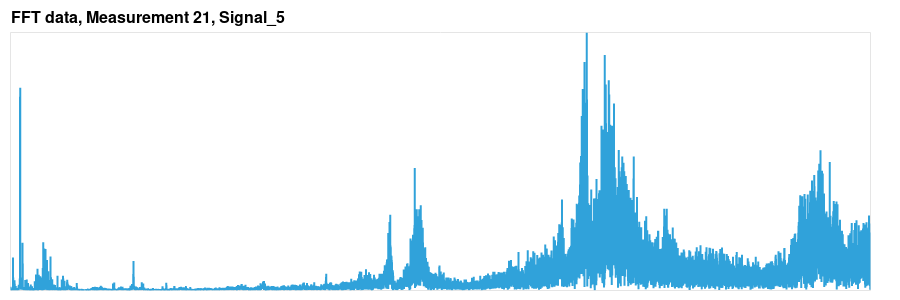
\includegraphics[width=\textwidth]{figures/Signal_5_fft_example.png}
\caption{Signal 5 fft example}
\label{fft_example}
\end{figure}

Es wird sich zeigen, dass der Algorithmus für die dünnbesetzte Hauptkomponentenanalyse sehr rechenintensiv sein kann. Daher haben wir uns entschieden, nur einen Teil der ursprünglichen Zeitreihe zu verwenden. Mithilfe einem Blick auf das Spektrogramm in Abbildung \ref{spectrogram} erkennen wir, dass sich die Frequenzen über den Messzeitraum kaum verändern. Dies ist darauf zurückzuführen, dass der Maschine konstant Material zugeführt wird. Daher können wir die Dimension um einen Faktor $100$ reduzieren ohne wichtige Informationen zu verlieren. Des Weiteren wurden Teile der Frequenzen, welche außerhalb des Frequenzbereichs des jeweiligen Sensors liegen, abgeschnitten. Somit verbleiben wir mit $p \approx 15,000$ Variablen. Um die Varianzen der Frequenzen vergleichbarer zu machen, haben wir die Daten ähnlich wie bei der klassischen Hauptkomponentenanalyse zentriert.

\begin{figure}
\centering
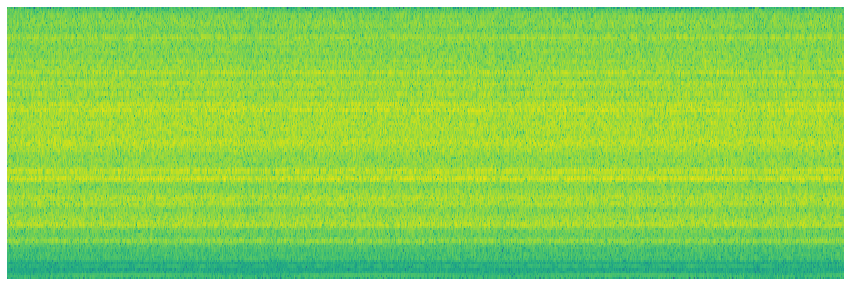
\includegraphics[width=\textwidth]{figures/Signal_5_time_frequency_change.png}
\caption{Signal 5 time frequency change}
\label{spectrogram}
\end{figure}

%----------------------------------------------------------------------------------------
%	Anwedung auf Frequenzdaten
%----------------------------------------------------------------------------------------


\section{Anwendung auf Frequenzdaten}
\label{application_frequency_data}

Unsere Implementierung ermöglicht eine Wahl verschiedene Parameter bezüglich des Modells bzw. des Algorithmus. Für eine Beschränkung der Laufzeit setzen wir eine maximale Anzahl an Iterationen von $500$ und eine Toleranz von $10^{-4}$. Falls nach $500$ Iterationen die vorgegebene Toleranz noch immer nicht erreicht ist, werden wir dies im Folgenden kenntlich machen. Ein Modellparameter, den es zu wählen gilt, ist die Anzahl zu berechnender Hauptkomponenten. Wie bereits in \ref{spca_theorems} beschrieben, wird dazu meist das Ergebnis einer klassischen Hauptkomponentenanalyse verwendet. Es hat sich gezeigt, dass $2$ Hauptkomponenten für die meisten Sensoren ausreichen, um einen Großteil des Datensatzes zu erklären. Zu Analysezwecken haben wir uns dennoch entschieden einen Durchlauf mit $2$ und einen mit $10$ Hauptkomponenten zu starten. 

Interessanter ist die Wahl der Hyperparameter $\lambda$ und $\alpha$, welche wesentlichen Einfluss auf die Ergebnisse besitzen. Auch wenn prinzipiell die Möglichkeit besteht, differenzierte Bestrafungen je Hauptkomponente $\lambda_j$ auszuwählen, beschränken wir uns der Einfachheit halber auf eine einheitliche Bestrafung. Für die Wahl von $\lambda$ haben wir sowohl mehrere Werte ausprobiert, als auch eine Rastersuche bezüglich der in \ref{choice_of_tuning_parameters} beschriebenen BIC-Kriterien durchgeführt. Dafür verwenden wir auf einer log-Skala gleichverteilte Werte im Bereich zwischen $10^{-7}$ und $10^0$. Dagegen wählen wir für das Verhältnis zwischen Lasso und Ridge-Bestrafung die Werte $[0.1,\, 0.5,\, 0.7,\, 0.9,\, 0.95,\, 0.99,\, 1]$. Mithilfe des BIC-Kriteriums können wir zeitgleich über $\lambda$ und $\alpha$ optimieren. Es hat sich in den Anwendungen gezeigt, dass eine geeignete Liste für $\alpha$ mehr Werte nahe $1$ hat, da sich dort die größten Änderungen ergeben. Damit stärken wir den Lasso-Strafterm im Vergleich zum Ridge-Strafterm.

Exemplarisch werden wir uns nun mit einem der Beschleunigungssensoren weiter beschäftigen. An dieser Stelle möchten wir erwähnen, dass wir die Sensoren getrennt betrachten, d.h. die dünnbesetzte Hauptkomponentenanalyse auf die Sensoren einzeln anwenden. Dies ist aufgrund der Unterschiedlichkeit der Sensoren sinnvoll. Wir werden nun ausgewählte Ergebnisse vorstellen. 


%----------------------------------------------------------------------------------------
%	Auswertung der Ergebnisse
%----------------------------------------------------------------------------------------


\section{Auswertung der Ergebnisse}
\label{evaluation}

Im Rahmen dieser Arbeit können wir nun einen begrenzten Teil der Ergebnisse präsentieren. Ziel wird es sein, wesentliche Ergebnisse und Effekte des Algorithmus zu erläutern und gegebenenfalls weiter ins Detail zu gehen. 


%----------------------------------------------------------------------------------------
%	Klassische Analyse der Hauptachsen
%----------------------------------------------------------------------------------------


\subsection{Klassische Analyse der Hauptachsen}

Zunächst wollen wir eine klassische Analyse durchführen, wie sie oft für ein derartiges Verfahren gemacht wird. Um einen Vergleich zu ermöglichen, haben wir sowohl die klassische als auch die dünnbesetzte Hauptkomponentenanalyse durchgeführt. 

Für einen ersten Einblick in die Ergebnisse betrachten wir Abbildung \ref{sparse_pca_classical_analysis_pc_graph} bzw. \ref{sparse_pca_classical_analysis_sparse_pc_graph}, in welcher die ersten beiden Hauptkomponenten gegeneinander aufgezeichnet sind. Dies ist die Darstellung der Daten bezüglich der neu gefundenen Variablen. Zuerst wenden wir uns den Ergebnissen der klassischen Hauptkomponentenanalyse zu. Man sieht schnell, dass sich vier Gruppierungen ergeben. Durch die Transformation sehen wir eine deutliche Trennung zwischen Messungen mit und ohne Material, welche im Bild durch verschiedene Farben markiert sind. Des Weiteren sind die Messungen mit bzw. ohne Material in zwei Untergruppen geteilt. Die Unterschiede sind auf verschiedene Betriebszustände der Maschine zurückzuführen, auf welche wir hier nicht genauer eingehen können. Vergleichen wir dieses Ergebnis mit der dünnbesetzten Variante in Abbildung \ref{sparse_pca_classical_analysis_sparse_pc_graph}, erkennen wir viele Gemeinsamkeiten. Es treten dieselben Gruppierungen wie zuvor auf, so dass noch immer eine Trennung der Messungen bezüglich der Befüllung möglich ist. Ein kleinerer Unterschied ist in der zweiten Hauptkomponenten zu sehen, da bei der dünnbesetzten Variante drei Messungen noch stärker separiert werden.

Nun gilt es, das Zustandekommen dieses Bildes zu erklären. Wir wollen verstehen, warum wir eine Trennung zwischen Messungen bezüglich der Befüllung sehen. Vor allem interessieren wir uns dafür, welche Frequenzen für diesen Unterschied verantwortlich sind. Zu diesem Zweck betrachten wir Abbildung \ref{sparse_pca_classical_analysis_principal_axis} bzw. \ref{sparse_pca_classical_analysis_sparse_principal_axis}, in welcher die Hauptachsen der beiden Varianten zu sehen sind. Anhand der Hauptachsen können wir erkennen, welche Frequenzen eine entscheidende Rolle bei der Erhaltung der maximalen Varianz spielen. Demnach sind die größten Unterschiede im Datensatz auf die Frequenzen mit der größten Amplitude zurückzuführen. Auch wenn es in den niederen Frequenzen nicht leicht zu erkennen ist, sind bei der klassischen Hauptachse alle $\approx 15,000$ Einträge von Null verschieden sind. Eine Erklärung der beschriebenen Effekte ist hier quasi unmöglich. Wir können lediglich aussagen, dass die höheren Frequenzen in einer gewissen Weise wichtig sind. Genau hier liegt das Problem der klassischen Variante, denn eine Interpretation der Hauptachsen ist selten möglich. Es fließen einfach zu viele Koeffizienten in das Modell ein. Dagegen reduziert sich bei der dünnbesetzten Variante die Anzahl von Null verschiedener Einträge auf $\approx 40$ für $\lambda = 0.1$ und $\alpha = 0.1$. Durch die eingeschränkte Modellkomplexität erkennen wir drei Peaks im Frequenzspektrum. Im Wesentlichen sind also nur viel weniger Frequenzen für die beschriebene Trennung verantwortlich. Daher können wir folgern, dass genau diese Frequenzen durch die Maschine verursacht werden. Mit diesem Verfahren ist es also möglich Frequenzen zu identifizieren, welche eine klare Bedeutung im Kontext besitzen.

Zuletzt betrachtet man Abbildung \ref{sparse_pca_classical_analysis_scree_plot}, welche einen sog. \textit{scree plot} zeigt und oft als Bewertungsmittel von Dimensionsreduktionsverfahren dient. Mithilfe dieses Bildes kann man einsehen, welchen Anteil der Varianz des Datensatzes mit der niedrigdimensionalen Repräsentation erklärt wird. Zur Verdeutlichung der Effekte haben wir $10$ Hauptkomponenten berechnet. Es zeichnet sich ein klarer Varianzverlust je Hauptkomponente ab, wenn wir die dünnbesetzte Hauptkomponentenanalyse nutzen. Hier erhalten wir nur $25$\% der Information des Datensatz, während es im Gegensatz dazu $95$\% bei der klassischen Variante sind. Besonders deutlich wird der Kompromiss, den wir eingehen müssen. Dadurch, dass unsere Hauptachsen einfacher zu interpretieren sind, verlieren wir an erklärter Varianz. Ein geeignetes Maß zwischen Modellkomplexität und Rekonstruktionsfehler zu finden, kann von der Anwendung und der Intention abhängen. In unserem Fall ist die Möglichkeit einer Interpretation der Hauptachsen deutlich wichtiger als die Varianzerhaltung. Wir haben durch Abbildung \ref{sparse_pca_classical_analysis_pc_graph} bzw. \ref{sparse_pca_classical_analysis_sparse_pc_graph} gesehen, dass uns durch einen Rückgang der Varianz nicht zwangsläufig Informationen verloren gehen müssen. Wir konnten trotz geringer Varianz ein ähnliches Bild mit denselben Gruppierungen erzielen.

\begin{figure}
\centering
\begin{subfigure}{0.45\textwidth}
\centering
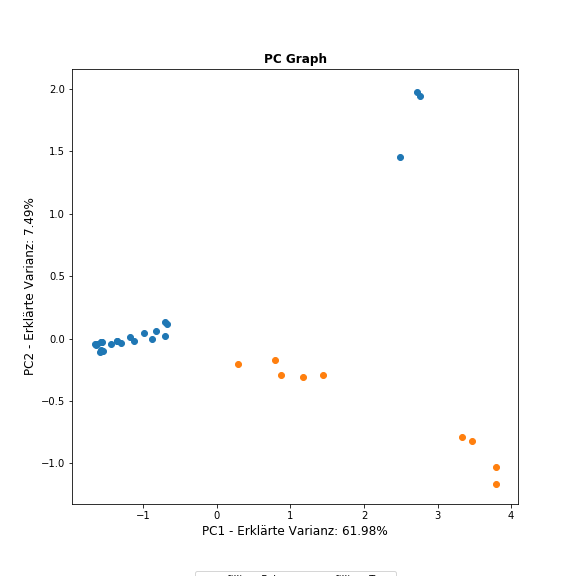
\includegraphics[width = \textwidth]{figures/Signal_5_pc_graph.png}
\caption{Signal 5 PC Graph}
\label{sparse_pca_classical_analysis_pc_graph}
\end{subfigure}
%
\begin{subfigure}{0.45\textwidth}
\centering
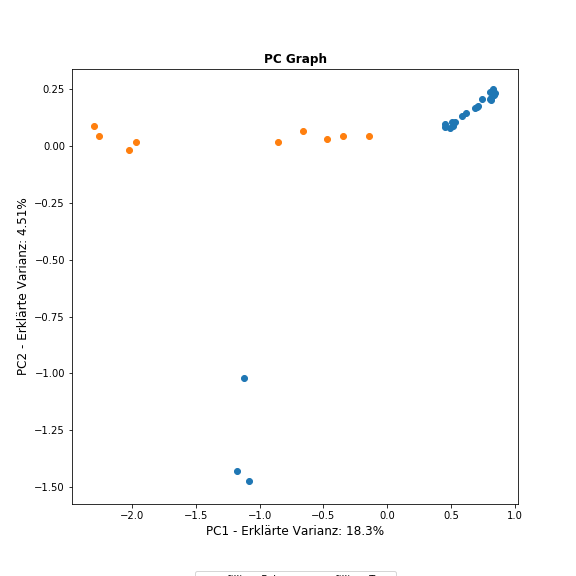
\includegraphics[width = \textwidth]{figures/Signal_5_sparse_pc_graph.png}
\caption{Signal 5 Sparse PC Graph}
\label{sparse_pca_classical_analysis_sparse_pc_graph}
\end{subfigure}
%
\begin{subfigure}{0.9\textwidth}
\centering
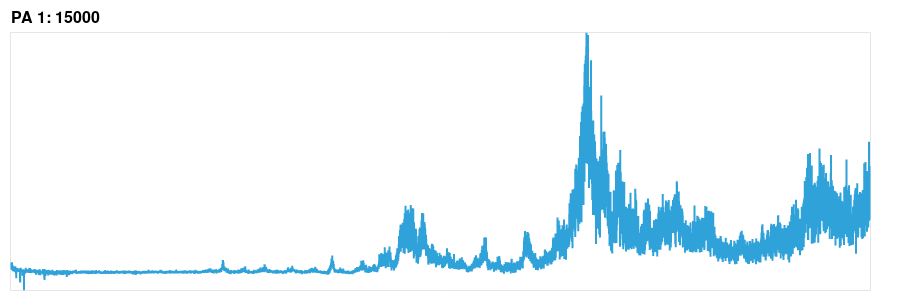
\includegraphics[width=\textwidth]{figures/Signal_5_principal_axis.png}
\caption{Signal 5 principal axis}
\label{sparse_pca_classical_analysis_principal_axis}
\end{subfigure}
%
\begin{subfigure}{0.9\textwidth}
\centering
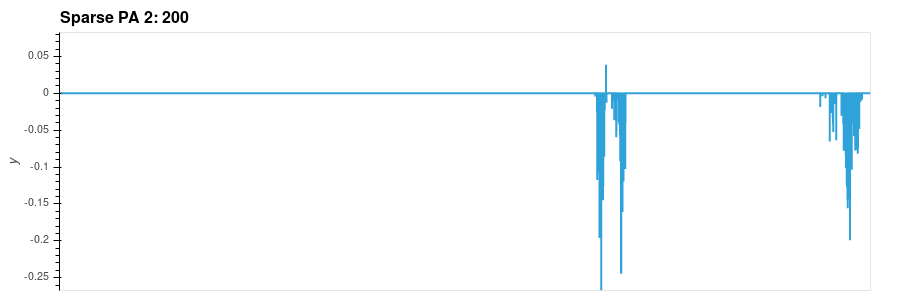
\includegraphics[width=\textwidth]{figures/Signal_5_sparse_principal_axis.png}
\caption{Signal 5 sparse principal axis}
\label{sparse_pca_classical_analysis_sparse_principal_axis}
\end{subfigure}
%
\begin{subfigure}{0.9\textwidth}
\centering
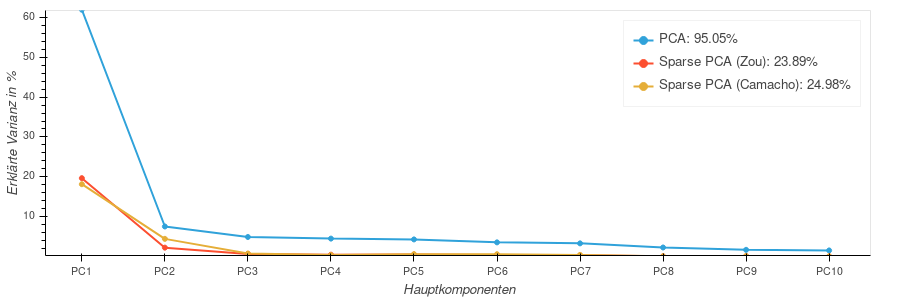
\includegraphics[width = \textwidth]{figures/Signal_5_scree_plot_10.png}
\caption{Signal 5 Scree Plot}
\label{sparse_pca_classical_analysis_scree_plot}
\end{subfigure}
\caption{Vergleich der klassischen mit der dünnbesetzten Hauptkomponentenanalyse für $\lambda=10^{-4}$ und $\alpha = 0.95$.}
\label{sparse_pca_classical_analysis}
\end{figure}


%----------------------------------------------------------------------------------------
%	Wahl der Hyperparameter
%----------------------------------------------------------------------------------------


\subsection{Wahl der Hyperparameter}

Im vorangegangenem Abschnitt haben wir beispielhaft gezeigt, wie die Ergebnisse einer dünnbesetzten Hauptkomponentenanalyse zu interpretieren sind. Für die Analyse haben wir bestimmte Werte von $\alpha$ und $\lambda$ vorgegeben, die möglichst gute Ergebnisse erzielen. Es stellt sich jedoch die Frage, wie sich die einzelnen Hauptachsen und Hauptkomponenten verändern, falls wir andere Werte für die Hyperparameter wählen. Zu diesem Zweck wenden wir uns Abbildung \ref{results_parameter_benchmark} zu. Hier haben wir die Anzahl an Hauptkomponenten fixiert und versucht, die Effekte in Abhängigkeit von $\lambda$ für einen akustischen Sensor zu beschreiben.

Abbildung \ref{results_parameter_benchmark_degrees_of_freedom} zeigt wie sich $\operatorname{df}(\lambda)$, also die Anzahl von Null verschiedener Einträge in den Hauptachsen, bei Veränderung von $\lambda$ bzw. $\alpha$ verhält. Klar erkennbar ist der relativ gleichmäßige Abfall der Freiheitsgrade, d.h. für wachsendes $\lambda$ werden unsere Hauptachsen zunehmend dünnbesetzt. Dies entspricht unseren Erwartungen aus Kapitel \ref{sparse_pca}. Verschieben wir das Verhältnis der Bestrafung von der $\ell_1$ zur $\ell_2$-Norm, sprich kleineres $\alpha$, steigt die Anzahl der Freiheitsgrade. Dies bestätigt, dass die $\ell_1$-Norm im Gegensatz zur $\ell_2$-Norm eine Dünnbesetzung hervorruft. Ab einem gewissem Punkt $\lambda \approx 10^{-2}$ für $\alpha > 0.5$ bzw. $\lambda \approx 10^{-1}$ für $\alpha = 0.1$ ist die Bestrafung zu stark, so dass die Hauptachsen dem Nullvektor entsprechen und keine Anpassung an den Datensatz mehr stattfindet.

Interessant ist nun, wie sich die erklärte Varianz des Datensatzes im Vergleich verhält, welche in Abbildung \ref{results_parameter_benchmark_explained_variance} zu sehen ist.  Auffällig ist, dass sich für $\lambda$ im Bereich von $[10^{-7}, 10^{-3}]$ kaum Änderungen in der Varianz ergeben. In diesem Bereich sind wir nur leicht unter dem Niveau der klassischen Variante. Im Umkehrschluss können wir aufgrund der kontinuierlichen Stagnation der Freiheitsgrade die Modellkomplexität verringern, aber zeitgleich den Rekonstruktionsfehler auf konstantem Niveau halten. Erst nahe $\lambda \approx 10^{-2}$ für $\alpha > 0.5$ bzw. bei $\lambda \approx 10^{-1}$ für $\alpha = 0.1$ zeichnet sich ein deutlicher Einbruch ab. Dieser ist dadurch zu erklären, dass die Hauptachsen dann dem Nullvektor entsprechen. Aus der Kombination der beiden Abbildungen können wir schließen, dass nur wenige Frequenzen wirklich wichtig zur Erklärung der Varianz des Datensatzes notwendig sind.

Um eine automatisierte Wahl von $\lambda$ und $\alpha$ zu ermöglichen, haben wir in Abschnitt \ref{choice_of_tuning_parameters} Vorgehensweisen mithilfe eines BIC-Kriteriums beschrieben. Eine Anwendung des Kriteriums nach \cite{croux, guo} befindet sich in Abbildung \ref{results_parameter_benchmark_bic}. Hier zeichnet sich ein Minimum im Bereich von $\lambda \in [10^{-4}, 10^{-3}]$ für $\alpha > 0.5$ bzw. nahe $\lambda \approx 10^{-2}$ ab, welches wir nach obiger Analyse erwarten konnten. Es wird also ein Punkt gewählt, an welchem die erklärte Varianz gerade noch auf sehr hohem Niveau, aber die Modellkomplexität gering ist. Letztere Abbildung ist also eine Kombination der Erkenntnisse und kann genutzt werden, um eine Balance zwischen Dünnbesetzung und erklärter Varianz zu finden. An dieser Stelle möchten wir erwähnen, dass die Resultate des BIC-Kriteriums nicht für alle Sensoren zufriedenstellend waren. Genauer gesagt sehen wir in manchen Fällen, dass die Gewichtung zwischen Modellkomplexität und Rekonstruktionsfehler nicht passend gewählt ist. Dies kann daran liegen, dass BIC-Kriterien in hochdimensionalen Fällen versagen können \cite{giraud}. Für unsere Zwecke wurden für die betroffenen Sensoren daher eine manuelle Gewichtung vorgenommen.

\begin{figure}
\centering
\begin{subfigure}{0.9\textwidth}
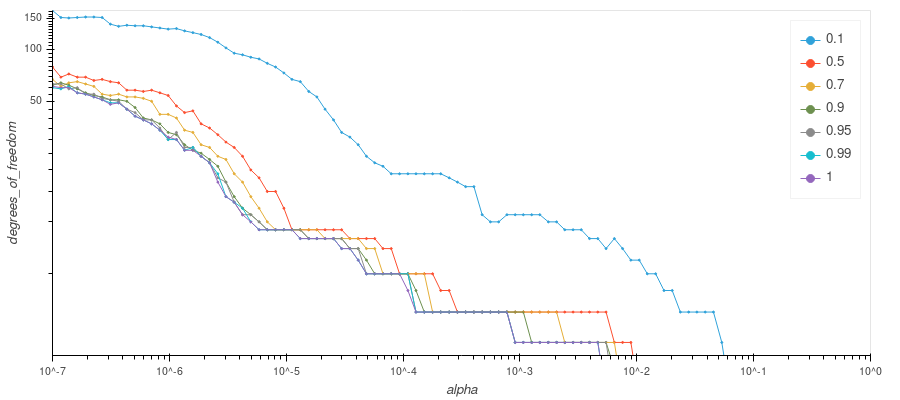
\includegraphics[width=\textwidth]{figures/Signal_0_degrees_of_freedom.png}
\caption{Anzahl Freiheitsgrade in Abhängigkeit von $\lambda$.}
\label{results_parameter_benchmark_degrees_of_freedom}
\end{subfigure}
%
\begin{subfigure}{0.9\textwidth}
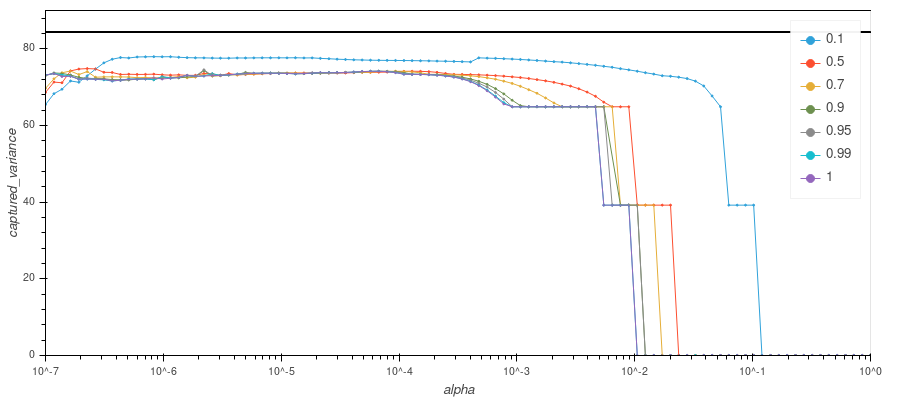
\includegraphics[width=\textwidth]{figures/Signal_0_explained_variances.png}
\caption{Erklärte Varianz des Datensatzes in Abhängigkeit von $\lambda$.}
\label{results_parameter_benchmark_explained_variance}
\end{subfigure}
%
\begin{subfigure}{0.9\textwidth}
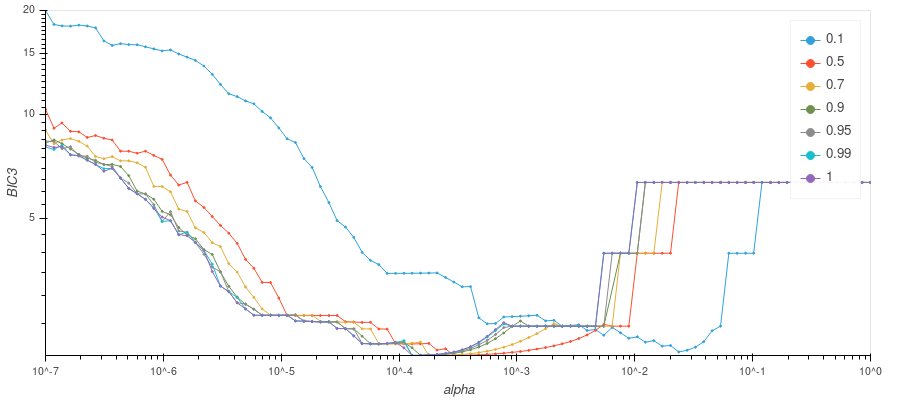
\includegraphics[width=\textwidth]{figures/Signal_0_bic.png}
\caption{Wahl der Hyperparameter mithilfe eines minimalen BIC-Kriteriums.}
\label{results_parameter_benchmark_bic}
\end{subfigure}
\caption{Die Abbildung zeigt wie sich eine Wahl der Hyperparameter $\alpha$ und $\lambda$ mithilfe eines BIC-Kriterium gestalten kann. Um Erkenntnisse über die Entstehung der BIC-Abbildung zu gewinnen, werden zusätzlich die beiden Komponenten Anzahl Freiheitsgrade und erklärte Varianz gezeigt. Zu beachten ist die logarithmische Skala für $\lambda$.}
\label{results_parameter_benchmark}
\end{figure}


%----------------------------------------------------------------------------------------
%	Verhalten des Algorithmus
%----------------------------------------------------------------------------------------


\subsection{Verhalten des Algorithmus}

Im Zuge dieser Arbeit möchten wir nicht nur die Ergebnisse einiger Experimente, sondern auch das Verhalten des Algorithmus an sich beschreiben. Dafür werden wir uns verschiedene Größen wie Laufzeit, Anzahl Iterationen und Toleranz ansehen. Um ein Gefühl für diese Größen bei der dünnbesetzten Hauptkomponentenanalyse zu bekommen, haben wir einen Überblick in Tabelle \ref{algorithm_analysis_table} erstellt. Interessant dabei ist vor allem die Abhängigkeit vom Hyperparameter $\lambda$. Je kleiner wir die Bestrafung wählen, desto länger dauert der Algorithmus und desto mehr Iterationen werden benötigt. Da bei kleinem $\lambda$ mehr von Null verschiedene Einträge in den Hauptachsen erlaubt werden, stimmt diese Beobachtung mit der Komplexität des Algorithmus von Abschnitt \ref{complexity} überein. Die meiste Zeit wird dabei nicht überraschend für das Lösen des Elastic Nets durch das Koordinatenabstiegsverfahren verwendet. Hingegen sind die Kosten für das Minimieren über $\mat A$ unabhängig von den Hyperparametern und im Wesentlichen durch eine Singulärwertzerlegung bestimmt, welche für diesen Datensatz in einem Bruchteil einer Sekunde gelöst werden kann. Ein Blick auf Tabelle REF zeigt die Ergebnisse eines Profilers und bestätigt unsere Erwartungen.

\setlength{\tabcolsep}{12pt}
\begin{table}
\centering
\begin{tabular}{cccc}
$\bm{\lambda}$ & \textbf{Laufzeit} & \textbf{Iterationen} & \textbf{Toleranz}\\\hline\addlinespace
$10^{-6}$ & $65235.76$ sec & $>500$ & $2.271780 \cdot 10^{-1}$\\
$10^{-5}$ & $9158.24$ sec & $>500$ & $4.132993 \cdot 10^{-4}$\\
$10^{-4}$ & $777.36$ sec & $99$ & $4.233382 \cdot 10^{-5}$\\
$10^{-3}$ & $201.49$ sec & $54$ & $5.531939 \cdot 10^{-5}$\\
$10^{-2}$ & $20.19$ sec & $5$ & $0$\\
$10^{-1}$ & $4.65$ sec & $1$ & $0$\\
\end{tabular}
\caption{Die Tabelle gibt einen Überblick über die Veränderung von Laufzeit, Iteration und Toleranz in Abhängigkeit von $\lambda$. Dabei wurde $\alpha=0.5$ und die Anzahl an Hauptkomponenten $k=10$ fest gewählt.\\Gerechnet wurde auf einem Intel Xeon Gold 6130F@2.10GHz.}
\label{algorithm_analysis_table}
\end{table}
\setlength{\tabcolsep}{6pt}

Logischerweise erhöht sich mit der Anzahl an Iterationen auch die Laufzeit des Algorithmus. Aus Tabelle \ref{algorithm_analysis_table} lässt sich aber nicht direkt erkennen, ob sich auch die Laufzeit je Iteration mit $\lambda$ verändert. In Abbildung \ref{run_time_per_iteration} beobachten wir auch eine Zunahme der Laufzeit je Iteration bei Senkung von $\lambda$ im Mittel. Des Weiteren steigt die Laufzeit, wenn mehr Gewicht auf eine Lasso-Bestrafung gelegt wird, also $\alpha$ nahe 1 gewählt wird.

Da wir eine maximale Anzahl von $500$ Iterationen festgelegt haben, kommt es bei Werten $\lambda < 10^{-5}$ zu einer erhöhten Toleranz. Eine Erhöhung der Anzahl an Iterationen kann die Toleranz verringern, jedoch steigt damit auch die Laufzeit. Diese Obergrenze scheint für unsere Anwendung eine sinnvolle Wahl zu sein, muss aber für jeden Datensatz geeignet angepasst werden. Denkbar sind auch schwächere Konvergenzkriterien, die gegebenenfalls die Laufzeit verringern können.

\begin{figure}
\centering
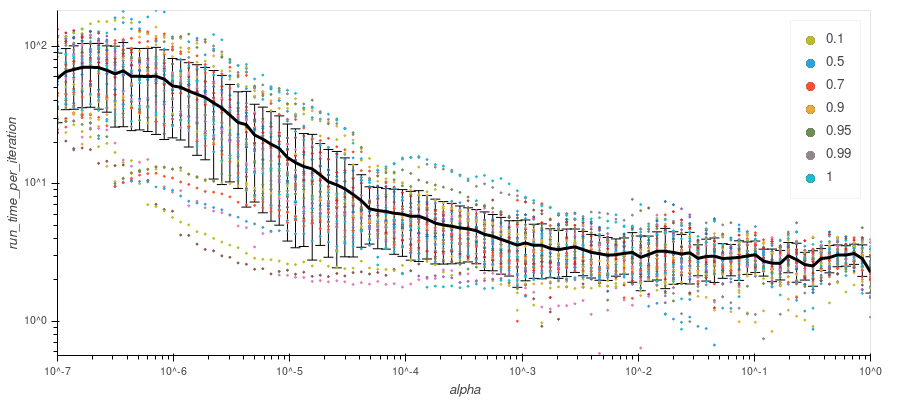
\includegraphics[width = 0.9\textwidth]{figures/run_time_per_iteration.png}
\caption{In dieser Abbildung ist die Laufzeit pro Iteration bei Veränderung des Hyperparameters $\lambda$ auf einer logarithmischen Skala zu sehen. Da auch $\alpha$ in unseren Experimenten variiert worden ist und mehrere Sensoren betrachtet werden, sehen wir mehrere Punkte je $\lambda$. Im Mittel klar zu erkennen ist ein Anstieg der Laufzeit bei Verringerung der Stärke der Bestrafung $\lambda$.}
\label{run_time_per_iteration}
\end{figure}


%----------------------------------------------------------------------------------------
%	Experimentelle Überprüfung der berechneten Varinanz
%----------------------------------------------------------------------------------------


\subsection{Experimentelle Überprüfung der berechneten Varianzen}

In Abschnitt \ref{adjustment_of_variances} haben wir unterschiedliche Wege zur Berechnung der Hauptkomponenten und deren erklärte Varianz gezeigt. Um die Arbeit von Camacho et al. \cite{camacho} experimentell zu überprüfen, werden wir vier Kriterien definieren, welche auf den unterschiedlichen Vorgehensweisen basieren. Für jede dieser wird die Varianz der Residuen addiert und mit der Gesamtvarianz des Datensatzes normalisiert.
\begin{itemize}
\item TotQR: $\quad \frac{\sum_{j=1}^k R_{jj}^2 + \spur{\mat E^T\mat E}}{\spur{\mat X^T\mat X}} \quad$ (Vorgehensweies Zou et al.)
\item TotZB: $\quad \frac{\spur{\mat B \mat Z^T \mat Z \mat B^T} + \spur{\mat E^T\mat E}}{\spur{\mat X^T\mat X}} \quad$ (Vorgehensweise Camacho et al.)
\end{itemize}
Bezüglich der Notation haben wir uns an Abschnitt \ref{adjustment_of_variances} gehalten. Zwei weitere Kriterien TotQR* und TotZB* ergeben sich durch die Korrektur der Hauptkomponenten mit der Moore-Penrose-Inverse $\mat Z^* = \mat X \mat B^T (\mat B^T\mat B)^+$. Falls alle Vorgehensweisen korrekt sind, können wir erwarten, dass jedes Kriterium den Wert $1$ hat. In Abbildung \ref{total_variance_validation} haben wir die Kriterien für unsere Experimente berechnet. Klar zu sehen ist, dass ohne eine Korrektur mit der Moore-Penrose-Inversen beide Varianten für die Varianzberechnung im Allgemeinem falsch sind. Auch wenn wir die Hauptkomponenten korrigieren, liefert die QR-Zerlegung keine richtigen Ergebnisse. Nur TotZB* hat in allen Fällen den Wert $1$ und ist damit der einzig korrekte Weg, Hauptkomponenten und Varianzen zu berechnen. Die von Zou et al. \cite{zou_sparsepca} vorgeschlagenen Varianten sind also falsch und sollten nicht verwendet werden. Somit können wir die Erkenntnisse aus \cite{camacho} experimentell bestätigen.

\begin{figure}
\centering
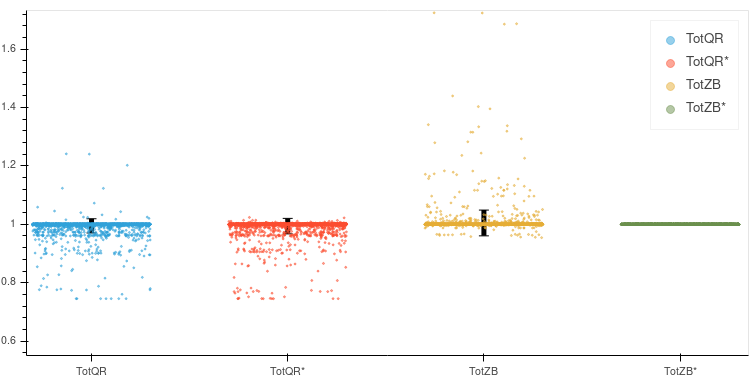
\includegraphics[width = 0.9\textwidth]{figures/total_variance_validation.png}
\caption{Zu sehen sind die Ergebnisse der unterschiedlichen Vorgehensweise bei der Berechnung der Hauptkomponenten und erklärter Varianzen. Nur die von Camacho et al. vorgeschlagene Variante TotZB* errechnet diese korrekt. Jeder Punkt entspricht eines unserer Experimente wie in Abschnitt \ref{application_frequency_data} beschrieben.}
\label{total_variance_validation}
\end{figure}
% Main chapter title
\chapter{Fazit}

% Chapter label
\label{conclusion}

Im Zuge dieser Arbeit haben wir die Konstruktion, Theorie und Anwendung der dünnbesetzten Hauptkomponentenanalyse detailliert erläutert.
Nach einer kurzen Einführung in die Thematik und deren Relevanz in der Praxis haben wir uns mit den mathematischen Grundlagen des Verfahrens beschäftigt. Besonders wichtig waren Kenntnisse aus der linearen Algebra und verallgemeinerter Regressionsmodelle. Anschließend wurde das wohl weitverbreiteste Dimensionsreduktionsverfahren, die Hauptkomponentenanalyse, in verschiedenen Formen vorgestellt. Grenzen, mögliche Erweiterungen und theoretische Aussagen des klassischen Verfahrens wurden beschrieben, um ein umfassendes Bild zu vermitteln. Im weiteren Verlauf wurde ein Kernproblem herausgestellt, was zur Idee der dünnbesetzten Hauptkomponentenanalyse führte. Zu diesem Zweck wurde ein in der Literatur vorgeschlagener Ansatz detailliert erklärt und eine numerische Lösung entwickelt. Mithilfe einer eigenen Implementierung haben wir die dünnbesetzte Hauptkomponentenanalyse auf einen realen Datensatz angewandt. Die beachtlichen Ergebnisse wurden kritisch hinterfragt und validiert. Darüber hinaus haben wir herausgearbeitet, wie das Verfahren in der Praxis einzusetzen ist.


%----------------------------------------------------------------------------------------
%	Diskussion
%----------------------------------------------------------------------------------------


\section{Diskussion}

Wir besitzen nun ein sehr gutes Verständnis über die Rolle der Dünnbesetzung und deren Einsatz für die Entwicklung transparenter Modelle. Allerdings gibt es noch immer Details und Zusammenhänge, welche es näher zu verstehen gilt. So ist man für die dünnbesetzte Hauptkomponentenanalyse noch immer auf der Suche nach Kriterien, welche eine automatisierte Wahl der Modellparameter ermöglichen. Teilweise mussten wir in unserer Anwendung manuelle Gewichtungen vornehmen, um brauchbare Ergebnisse zu erzielen. An dieser Stelle ist die Verwendung weiterer Kriterien aus der Informationstheorie denkbar. Vorerst sind wir aber dazu angehalten eigene Analysen durchzuführen und automatisierte Kriterien kritisch zu hinterfragen.

In Kapitel \ref{relaxation} haben wir erwähnt, dass es durchaus andere Wege gibt, das Problem der dünnbesetzten Hauptkomponentenanalyse zu relaxieren. Allgemein gibt es leider keinen besten Weg bzw. einen besten Algorithmus, so dass eine Wahl situationsabhängig getroffen werden muss. Bislang haben wir keine Kritik an dem von uns vorgestellten Ansatz durch Zou et al. \cite{zou_sparsepca} geäußert. Jedoch gibt es auch hier Schwierigkeiten, die bei der Verwendung zu beachten sind. 

Im Vergleich zu anderen Methoden produziert der Algorithmus stärker korrelierte Hauptkomponenten. In der Praxis wäre es aber wünschenswert, wenn jede Hauptkomponente eine eigene Bedeutung im Kontext besitzt. Durch die Korrektur der Hauptkomponenten mit der Moore-Penrose-Inversen, wie es in \cite{camacho} vorgeschlagen wurde, wird eine Verringerung der Korrelation erreicht. Folglich ist das Niveau der Korrelation mit anderen Methoden vergleichbar. 

Weitere Kritik bezieht sich auf die Art der Modellierung. Das Sparse-PCA-Kriterium aus Kapitel \ref{sparse_pca} ist ein Optimierungsproblem über zwei Matrizen $\mat A$ und $\mat B$. Da sowohl $\mat A$ durch die Orthogonalitätsbedingung als auch $\mat B$ durch die verschiedenen Strafterme eingeschränkt ist, fehlt es dem Modell an Flexibilität. Je nach Stärke der Bestrafungen können wir daher nie die gesamte Varianz des Datensatzes erklären. Des Weiteren sind die dünnbesetzten Hauptachsen nicht wie üblich normalisiert. Zou et al. normalisieren die Hauptachsen daher am Ende des Algorithmus. Allerdings müsste die Matrix $\mat A$ dementsprechend angepasst werden, was in ihrer Arbeit nicht berücksichtigt wird und zu einem hohen Rekonstruktionsfehler führen kann. Daran erkennen wir, dass die Autoren primär an den dünnbesetzten Hauptachsen interessiert waren. Andere Verfahren erlauben eine flexiblere Modellierung, erreichen aber nicht immer eine vergleichbare Dünnbesetzung oder Laufzeit. Es fehlt der Literatur an einem weitreichendem Vergleich der verschiedenen Methoden in der Praxis.


%----------------------------------------------------------------------------------------
%	Ausblick
%----------------------------------------------------------------------------------------


\section{Ausblick}

In unserer Implementierung des Algorithmus haben wir bereits eine Verbesserung der Laufzeit gegenüber der von Zou et al. für hochdimensionale Datensätze erreicht. Wir können den Algorithmus weiter beschleunigen, indem wir einen Teil parallelisieren. Zwar müssen die Iterationen hintereinander ausgeführt werden, jedoch kann das Elastic Net Subproblem für jede Hauptachse unabhängig voneinander berechnet werden. Mithilfe dieser Parallelisierung ist es möglich noch bessere Laufzeiten in der Praxis zu erhalten.

Auch wenn algorithmische Reduktionen in der theoretischen Informatik häufig genutzt werden, bleiben sie im Bereich des maschinellen Lernens oft unberücksichtigt. In unserem Fall ist es tatsächlich möglich, das Elastic Net auf ein anderes weitverbreitetes überwachtes Lernverfahren zurückzuführen, eine sog. \textit{Support Vector Machine (SVM)}. Diese kommen sehr häufig für Mustererkennung bzw. Klassifikation der Beobachtungen in einem Datensatz zum Einsatz. In \cite{zhou} wird gezeigt, dass zu jeder Elastic Net Instanz ein binäres Klassifikationsproblem konstruiert werden kann, so dass die trennende Hyperebene eine identische Lösung nach Skalierung liefert. Dies ermöglicht die Nutzung schneller parallelisierter CPU/GPU-basierter SVM-Löser. Dadurch lässt sich in der Praxis eine um zwei Größenordnungen bessere Laufzeit erreichen. Für eine zukünftige Nutzung des von uns implementierten Algorithmus kann es daher sinnvoll sein, eine derartige Reduktion zu nutzen.



%----------------------------------------------------------------------------------------
%	THESIS CONTENT - APPENDICES
%----------------------------------------------------------------------------------------

\appendix % Cue to tell LaTeX that the following "chapters" are Appendices

% Include the appendices of the thesis as separate files from the Appendices folder
% Uncomment the lines as you write the Appendices

% Appendix A

\chapter{Frequently Asked Questions} % Main appendix title

\label{AppendixA} % For referencing this appendix elsewhere, use \ref{AppendixA}

\section{How do I change the colors of links?}

The color of links can be changed to your liking using:

{\small\verb!\hypersetup{urlcolor=red}!}, or

{\small\verb!\hypersetup{citecolor=green}!}, or

{\small\verb!\hypersetup{allcolor=blue}!}.

\noindent If you want to completely hide the links, you can use:

{\small\verb!\hypersetup{allcolors=.}!}, or even better: 

{\small\verb!\hypersetup{hidelinks}!}.

\noindent If you want to have obvious links in the PDF but not the printed text, use:

{\small\verb!\hypersetup{colorlinks=false}!}.

%\include{Appendices/AppendixB}
%\include{Appendices/AppendixC}

%----------------------------------------------------------------------------------------
%	BIBLIOGRAPHY
%----------------------------------------------------------------------------------------

\printbibliography[heading=bibintoc]

%----------------------------------------------------------------------------------------

\end{document}  
